\chapter{Metodologias propostas}\label{chap3}

Nesse capítulo as três metodologias para avaliação de incerteza em modelos geológicos multi-categóricos usando funções distâncias assinaladas propostas nessa tese são apresentadas. Todos os métodos são acompanhados de uma prova de conceito no banco de dados \textit{Swiss Jura} e um estudo de caso. 

\section{Parametrização do suporte do \textit{kernel}}\label{kernel_fac}

Esse método é uma adaptação do condicionamento das amostras apresentado no \autoref{chap:cond_amo}, para que tenha sua aplicação estendida para múltiplos domínios. No método proposto por \citeonline{mclennanstationarity} o interpolador é o inverso da distância já que outros interpoladores, como a krigagem, podem gerar pesos negativos que interferem na ponderação gerada pelo condicionamento das amostras.

Essa adaptação propõe, no lugar de modificar o peso dado às amostras, modificar o suporte dos \textit{kernels} usados na interpolação por funções de bases radiais multiplicando-os por um fator menor (pessimista) ou maior (otimista) que um. Para cada propriedade de função distância assinalada que representa cada categoria do depósito mineral, os cenários otimista, pessimista e caso base são gerados e combinados para criar múltiplos cenários para o modelo geológico multi-categórico.

Considere o exemplo em uma dimensão da \autoref{one_dim_ex}. A figura mostra quatro amostras, duas azuis que não pertencem ao domínio sendo modelado, e duas vermelhas que pertencem ao domínio sendo modelado. As amostras estão, da esquerda para a direita, nas posições 1, 10, 70 e 90.

\begin{figure}[H]
	\caption{\label{one_dim_ex} Amostras em posição 1, 10, 70 e 90. Amostras em azul não pertencem ao domínio enquanto amostras vermelhas pertencem.}
	\centering
		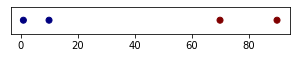
\includegraphics[width=0.4\textwidth]{capitulo_3/imagens/pointssd.png}
\end{figure}

A \autoref{uni_rbf} mostra, no gráfico na posição inferior, as amostras da \autoref{one_dim_ex} e no eixo y do gráfico, na posição superior, o valor da função distância assinalada calculada para cada uma das quatro amostras. A Figura \autoref{at} mostra uma função RBF com suporte igual a 25 centrada em cada uma das amostras. A Figura \autoref{dt} mostra, em preto, a superfície interpolada a partir da combinação linear das quatro RBFs após o cálculo dos pesos a partir do sistema de equações apresentado na \autoref{rbf_sist}. O limite entre os domínios é onde a distância assinalada interpolada é igual a zero.

\begin{figure}[H] 
    \centering
    \caption{Amostras em uma dimensão no gráfico na posição inferior e distâncias assinaladas calculadas para cada uma das amostras no eixo y do gráfico na posição superior.} \label{uni_rbf}
     \subfloat[][Uma RBF com suporte igual a 25 e centrada em cada uma das amostas.]{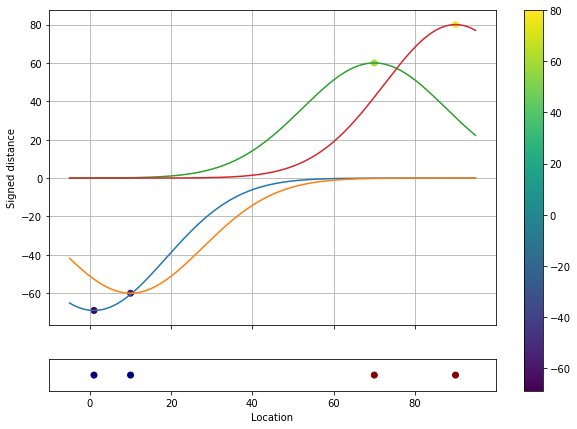
\includegraphics[width=.45\textwidth]{capitulo_3/imagens/RBF_before_train.png}\label{at}}
     \hspace{1em}
     \subfloat[][Uma RBF com suporte igual a 25 e centrada em cada uma das amostas após o cálculo dos pesos e sua combinação linear em preto.]{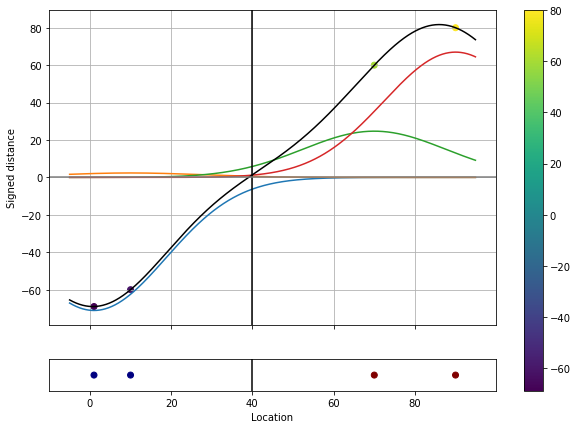
\includegraphics[width=.45\textwidth]{capitulo_3/imagens/RBF_after_train.png}\label{dt}}
\end{figure}

O método proposto modifica o suporte de uma cada uma das RBFs centradas nas amostras de acordo com o valor da distância assinalada calculada para aquela amostras a partir das curvas de parametrização mostradas na \autoref{param}. Dessa forma, cada RBF terá um suporte diferente. O volume do sólido fruto da extração da iso-superfĩcie zero, gerado pelo cenário otimista é maior do que o gerado pelo caso baso enquanto o volume do sólido gerado pelo caso pessimista é menor.

\begin{figure}[H] 
    \centering
    \caption{Parametrização das amostras.} \label{param}
     \subfloat[][Linear.]{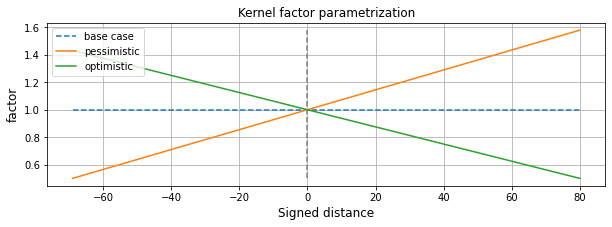
\includegraphics[width=.8\textwidth]{capitulo_3/imagens/linear_kfp.png}\label{paramlinear}} \\
     \subfloat[][Quadrática.]{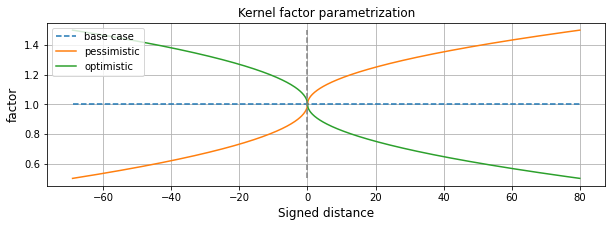
\includegraphics[width=.8\textwidth]{capitulo_3/imagens/quadratic_kfp.png}\label{paramquadrat}}
\end{figure}

A \autoref{dif_kernel} mostra as RBFs, que na \autoref{uni_rbf} apresentam suporte igual a 25, com seus suportes modificados a partir das curvas de parametrização lineares mostradas na Figura \autoref{paramlinear}. Os pesos são então calculados para cada um dos casos e uma superfície interpolada pode ser gerada a partir da combinação linear das RBFs.

\begin{figure}[H] 
    \centering
    \caption{Amostras em uma dimensão no gráfico na posição inferior e distâncias assinaladas calculadas para cada uma das amostras no eixo y do gráfico na posição superior..} \label{dif_kernel}
     \subfloat[][Caso otimista.]{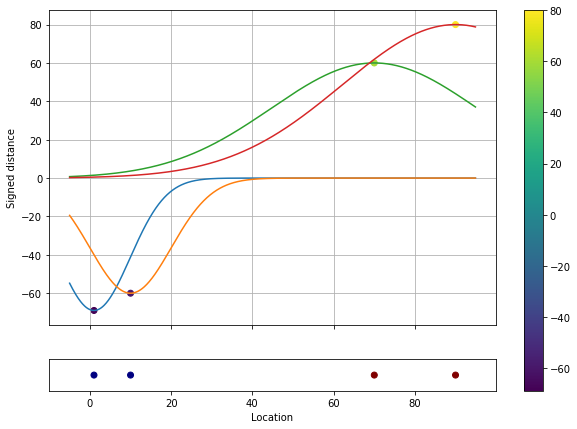
\includegraphics[width=.45\textwidth]{capitulo_3/imagens/pessimistic_kernels.png}\label{<figure1>}}
     \hspace{1em}
     \subfloat[][Caso pessimista.]{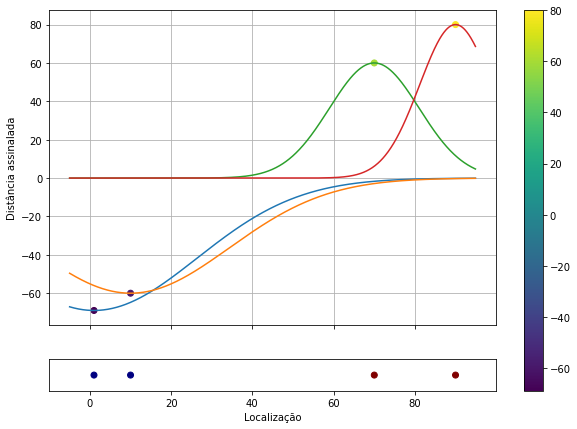
\includegraphics[width=.45\textwidth]{capitulo_3/imagens/optmistic_kernels.png}\label{<figure2>}}
\end{figure}

A \autoref{one_dim_result} mostra, em preto, a superfície interpolada para o caso base, em vermelho, para o cenário pessimista e em azul para o cenário otimista. 
 
\begin{figure}[H]
	\caption{\label{one_dim_result} Caso base e cenários otimista e pessimista para o exemplo unidimensional proposto.}
	\centering
		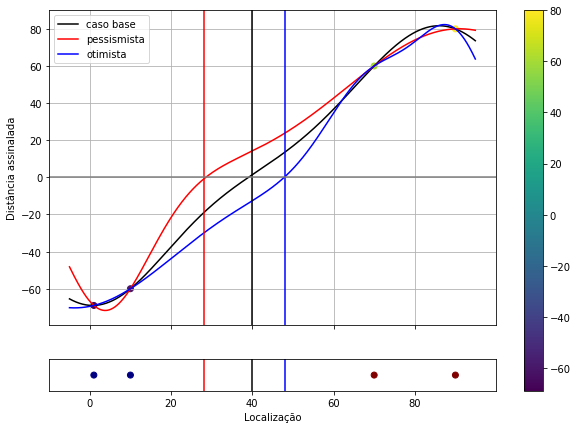
\includegraphics[width=0.6\textwidth]{capitulo_3/imagens/all_kernels.png}
\end{figure}

A aplicação do método no banco de dados \textit{Swiss Jura} consiste em, calcular as distâncias assinaladas para cada uma das cinco categorias do banco de dados. Então, os parâmetros para modificação do suporte devem ser escolhidos. Nesse caso, um modelo linear com valor de f mínimo igual a 0.95 para todas as categorias. A \autoref{quater_param} mostra as distâncias assinaladas para a categoria Quaternary interpoladas para o cenário pessimista, caso base e cenário otimista. Os mesmos cenários foram interpolados para as outras quatro categorias do banco de dados.

\begin{figure}[H] 
    \centering
    \caption{Distâncias assinaladas interpoladas para a categoria Quaternary do banco de dados \textit{Jura} para o caso base, e cenários pessimista e otimista.} \label{quater_param}
     \subfloat[][Caso pessimista.]{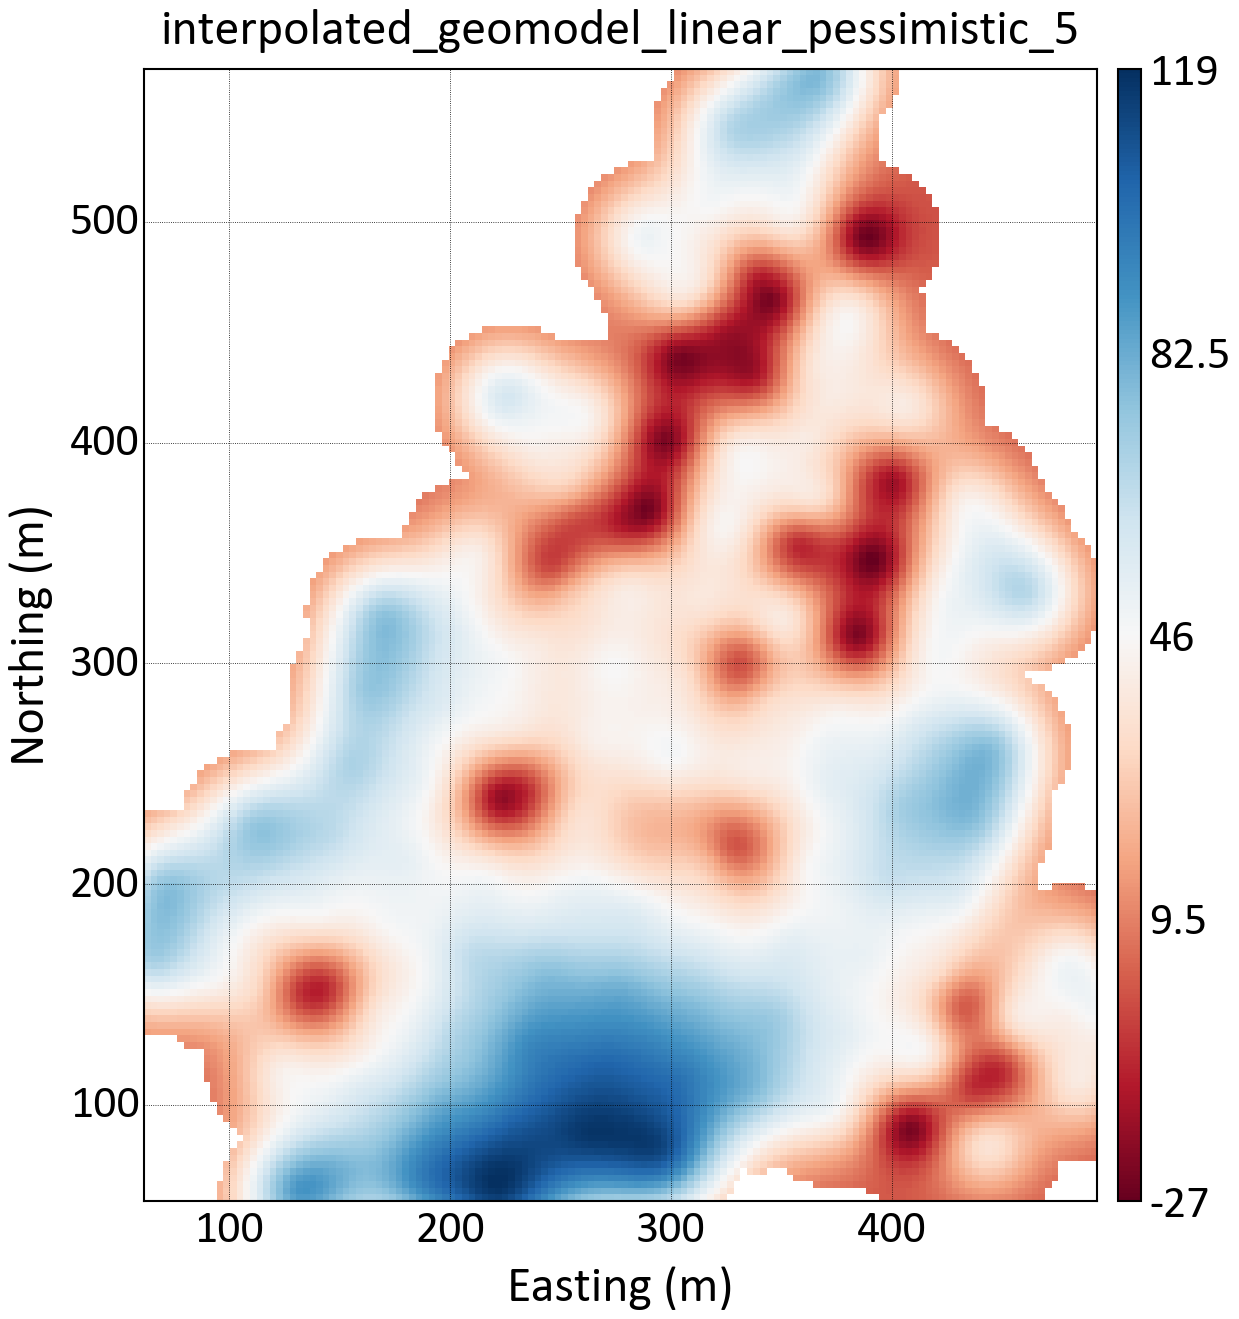
\includegraphics[width=.3\textwidth]{capitulo_3/imagens/pessimistic.png}\label{<figure1>}}
     \hspace{1em}
     \subfloat[][Caso base.]{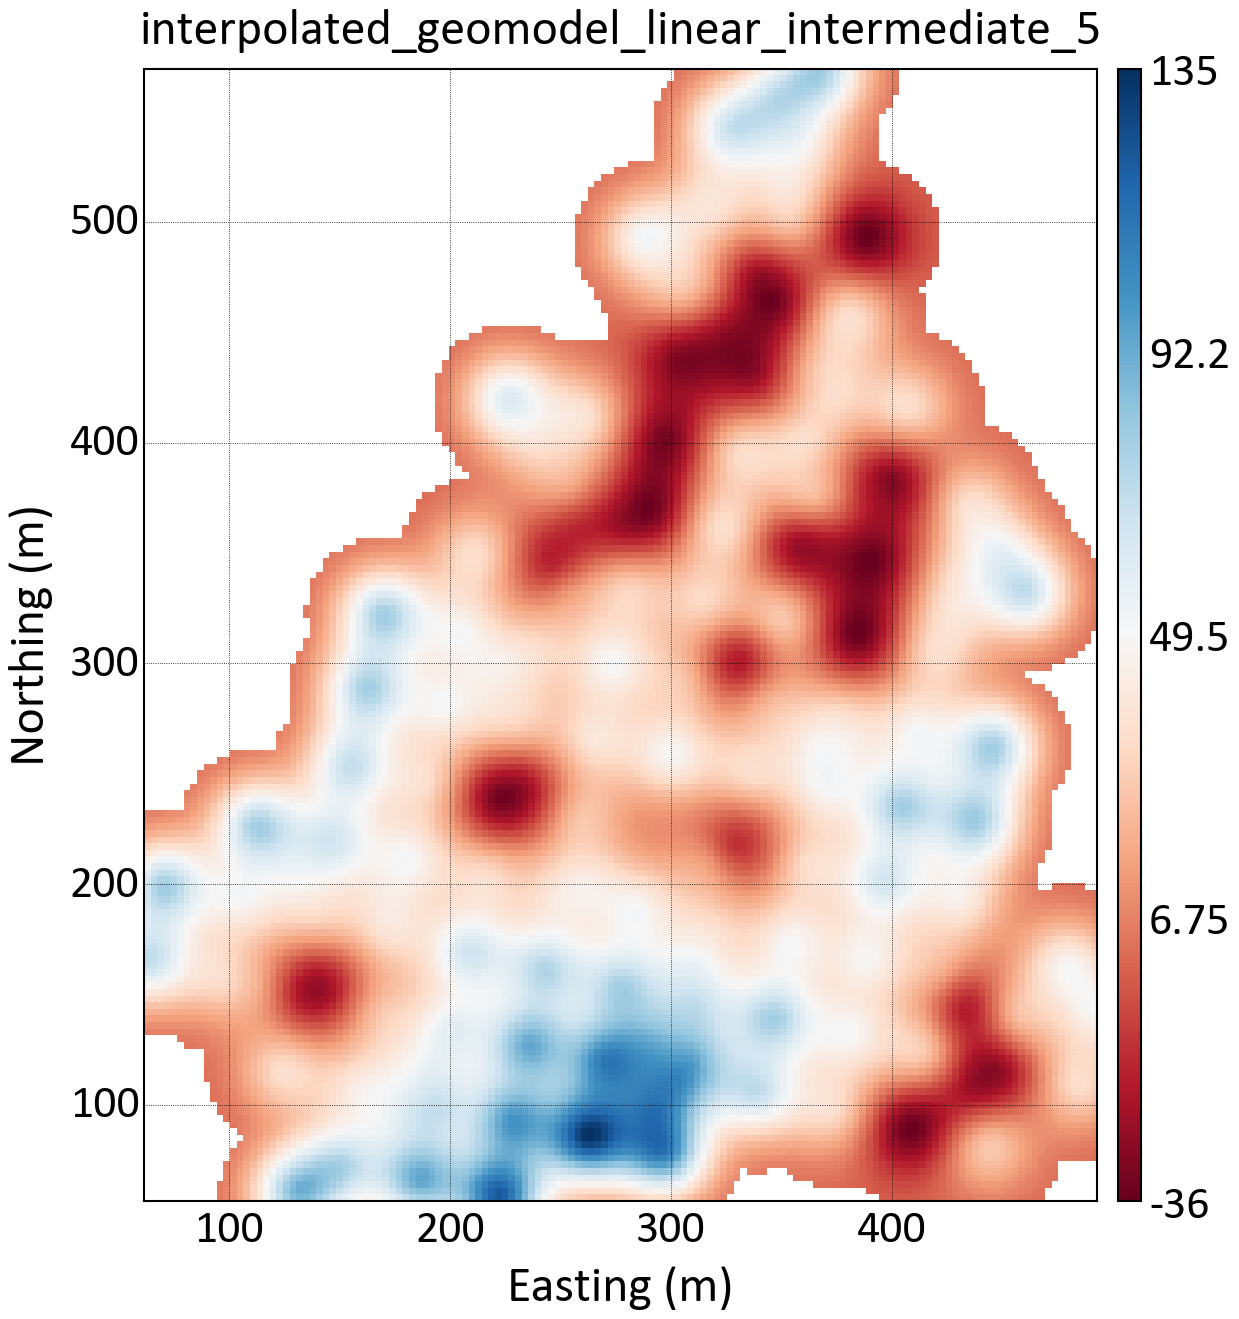
\includegraphics[width=.3\textwidth]{capitulo_3/imagens/intermediate.png}\label{<figure2>}}
     \hspace{1em}
     \subfloat[][Caso otimista.]{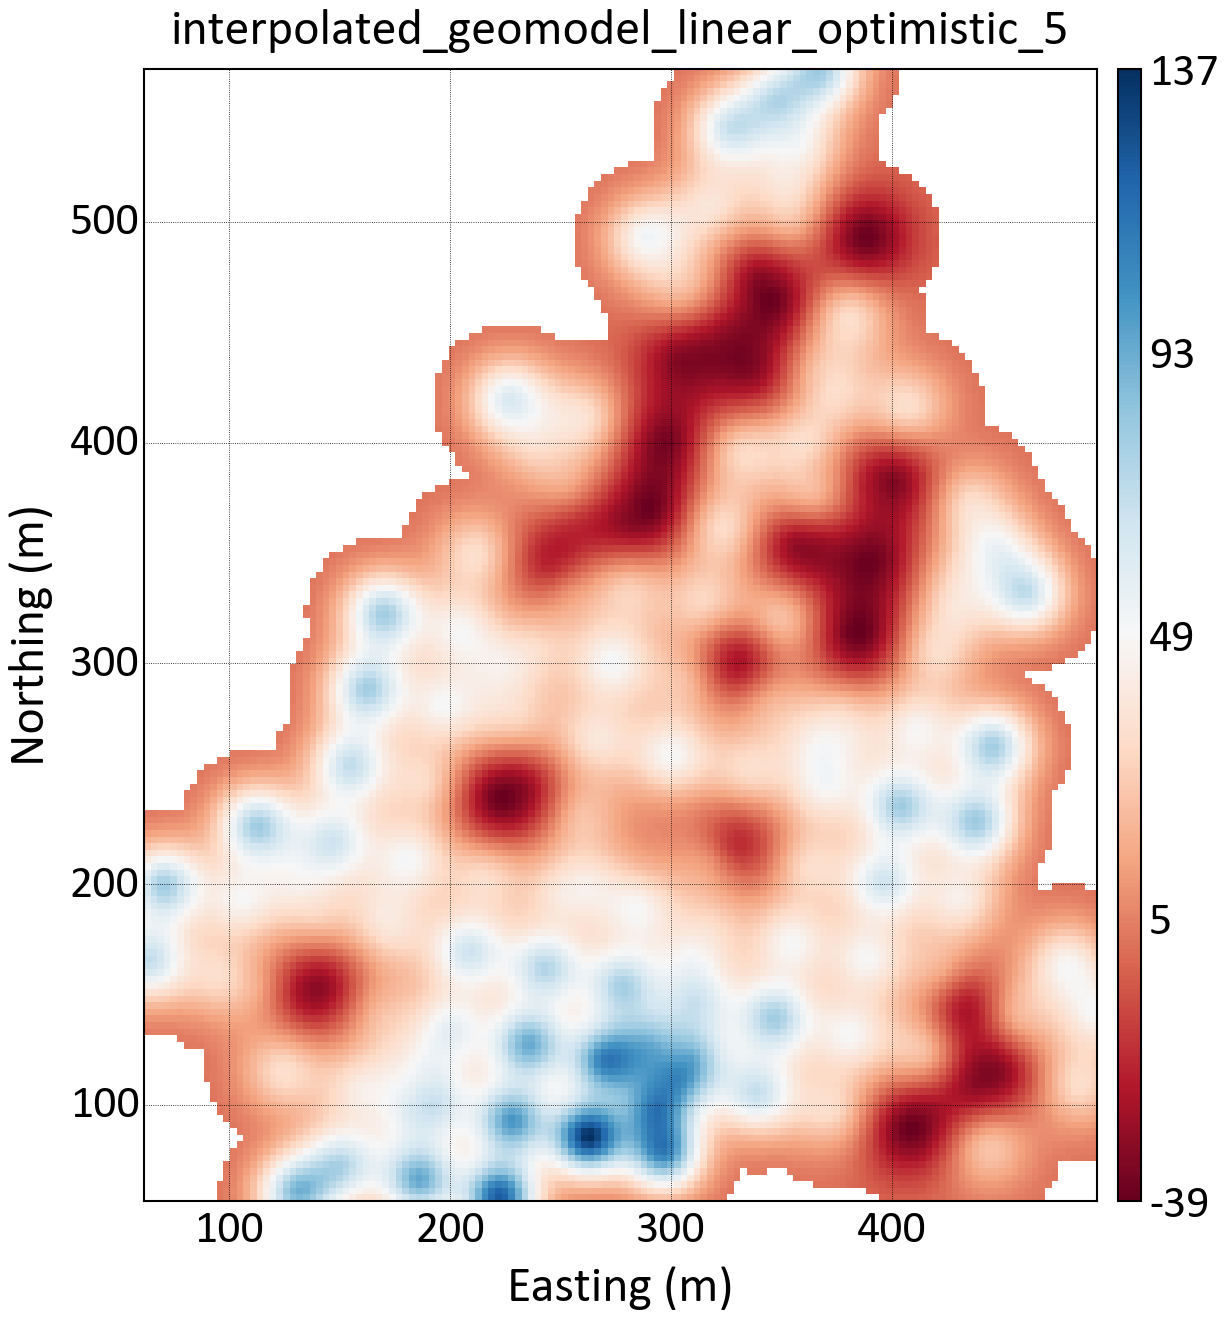
\includegraphics[width=.3\textwidth]{capitulo_3/imagens/optimistic.png}\label{<figure3>}}
\end{figure}

Para cada categoria há três diferentes cenários que devem ser combinados para criar os modelos geológicos multi-categóricos. Em alguns casos, a combinação do cenário otimista de uma categoria com grande área ou volume com o cenário pessimista de uma categoria de pequena área ou volume pode fazer com que nenhum bloco seja atribuído à menor categoria em alguns dos $3^K$ modelos gerados. Onde K é o número de categorias do banco de dados.  
Para contornar esse problema os modelos devem passar por um teste de reprodução dos dados amostrais. O algoritmo checa se o bloco com o centroide mais próximo a cada amostra foi classificado com a mesma categoria daquela amostra. O usuário seleciona um nível mínimo de reprodução, nesse caso 0.9. Desse modo, modelos que não reproduzem, pelo menos, 90\% dos dados amostrais são descartados. Dos 243 modelos gerados para o \textit{Swiss Jura} combinando os três cenários para as cinco diferentes categorias, 24 não foram descartados já que reproduzem, pelo menos, 90\% das amostras. 

A \autoref{jura_kernel} mostra duas realizações escolhidas aleatoriamente entre as 24 selecionadas, juntamente com as amostras representadas pelos círculos. Uma animação mostrando todas as realizações pode ser vista \href{https://github.com/robertorolo/kernel_support_parametrization_uncertainty_assess/blob/main/ezgif-7-b96e150c9939.gif}{aqui}.

\begin{figure}[H] 
    \centering
    \caption{Modelos geológicos para o \textit{Swiss Jura} criados a partir da parametrização do suporte do \textit{kernel}.} \label{jura_kernel}
     \subfloat[][Modelo 200.]{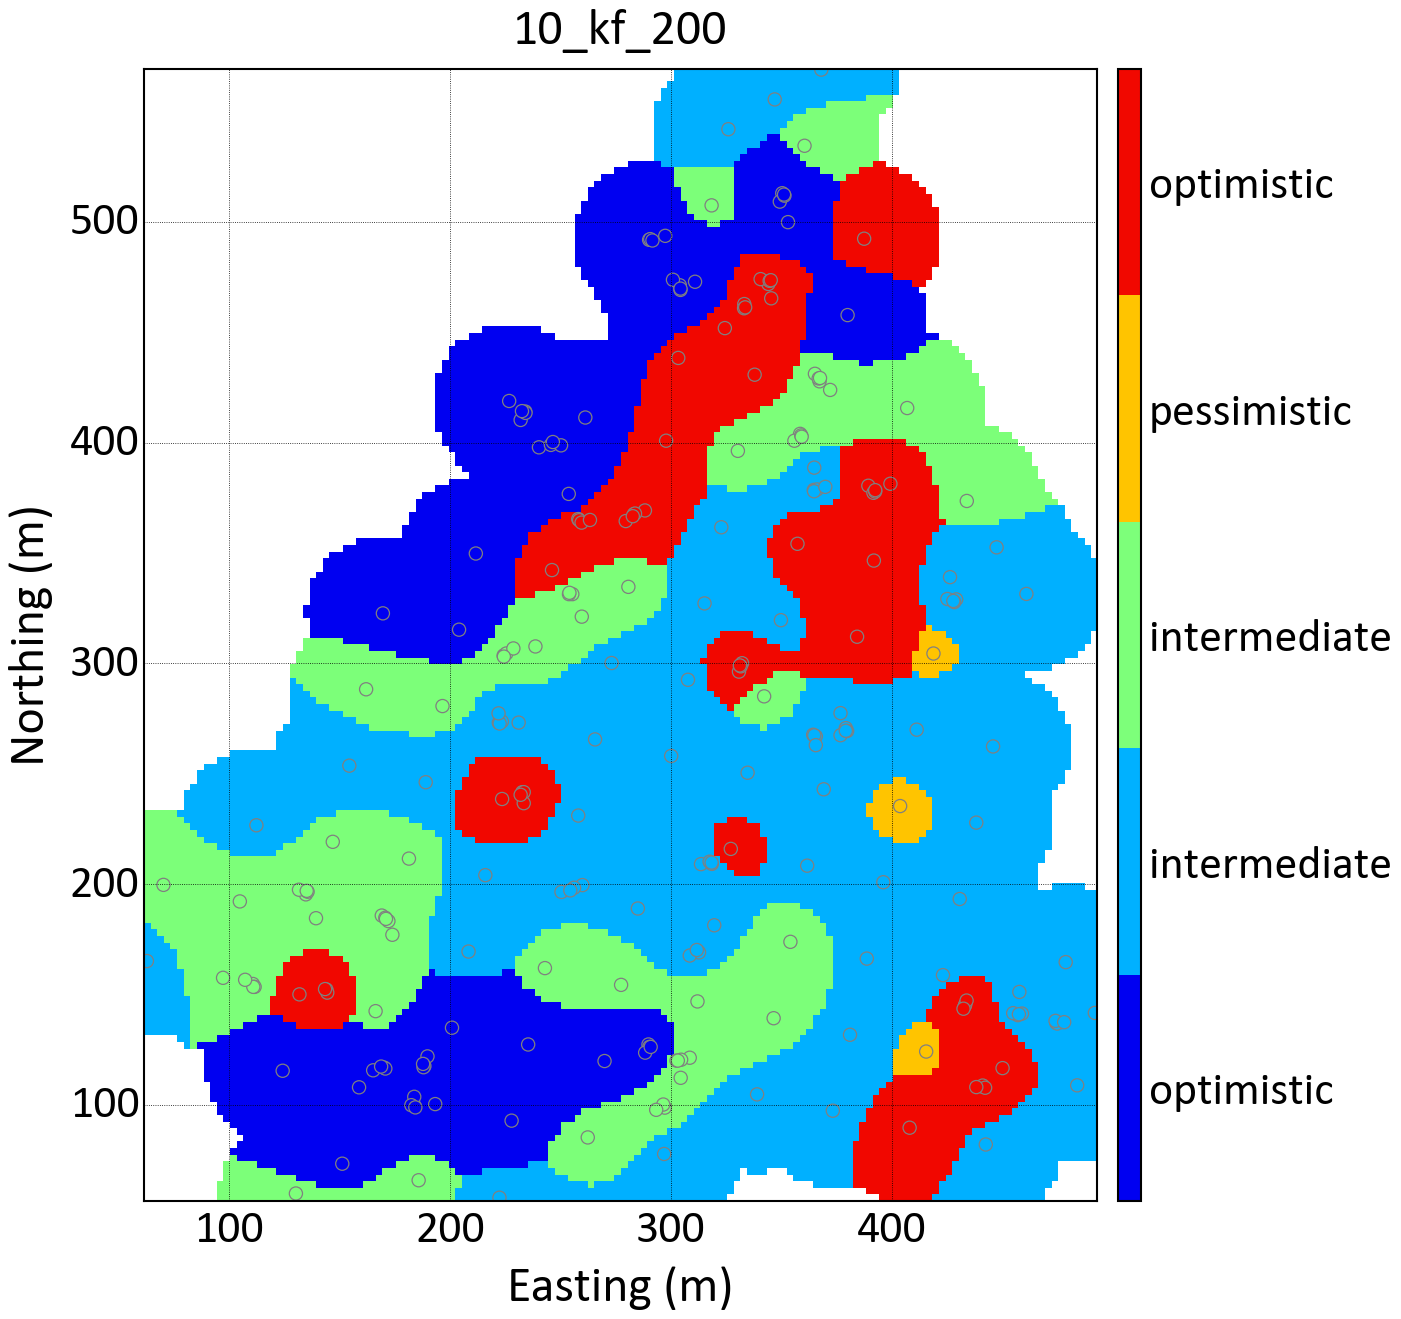
\includegraphics[width=.45\textwidth]{capitulo_3/imagens/out_model_10_kf_200.png}\label{<figure1>}}
     \hspace{1em}
     \subfloat[][Modelo 214.]{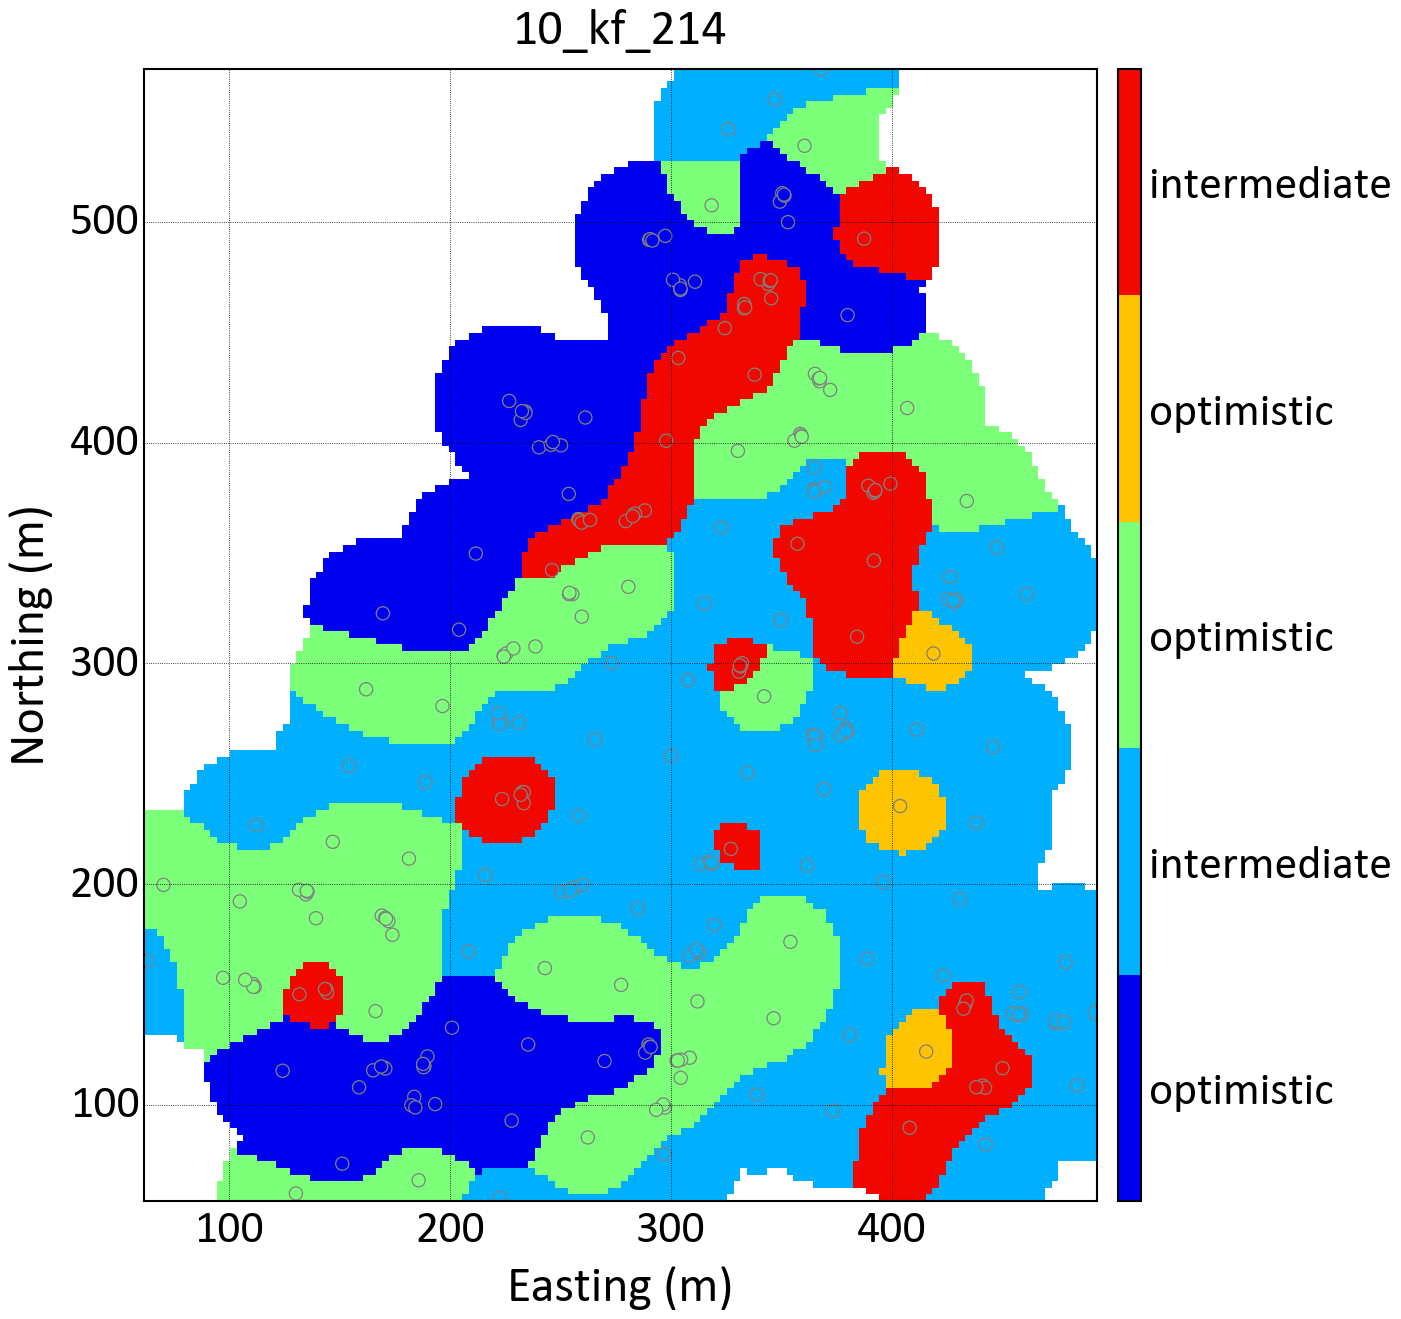
\includegraphics[width=.45\textwidth]{capitulo_3/imagens/out_model_10_kf_214.png}\label{<figure2>}}
\end{figure}

\subsection{Estudo de caso}

Pra ilustrar de forma prática a metodologia uma seção de um modelo conceitual foi produzida e é mostrada na Figura \autoref{exa}. O modelo é composto por rocha encaixante, mostrada em vermelho, um dique, mostrado em verde, e estruturas lenticulares, mostradas em azul.

O modelo conceitual exaustivo foi amostrado por 12 furos verticais igualmente espaçados. O espaçamento vertical das compostas é de 10 metros. Os furos verticais são mostrados na Figura \autoref{sampl}. 

\begin{figure}[H] 
    \centering
    \caption{Modelo conceitual composto por rocha encaixante, mostrada em vermelho, um dique, mostrado em verde, e estruturas lenticulares, mostradas em azul.} \label{concep_exhaust}
     \subfloat[][Exaustivo.]{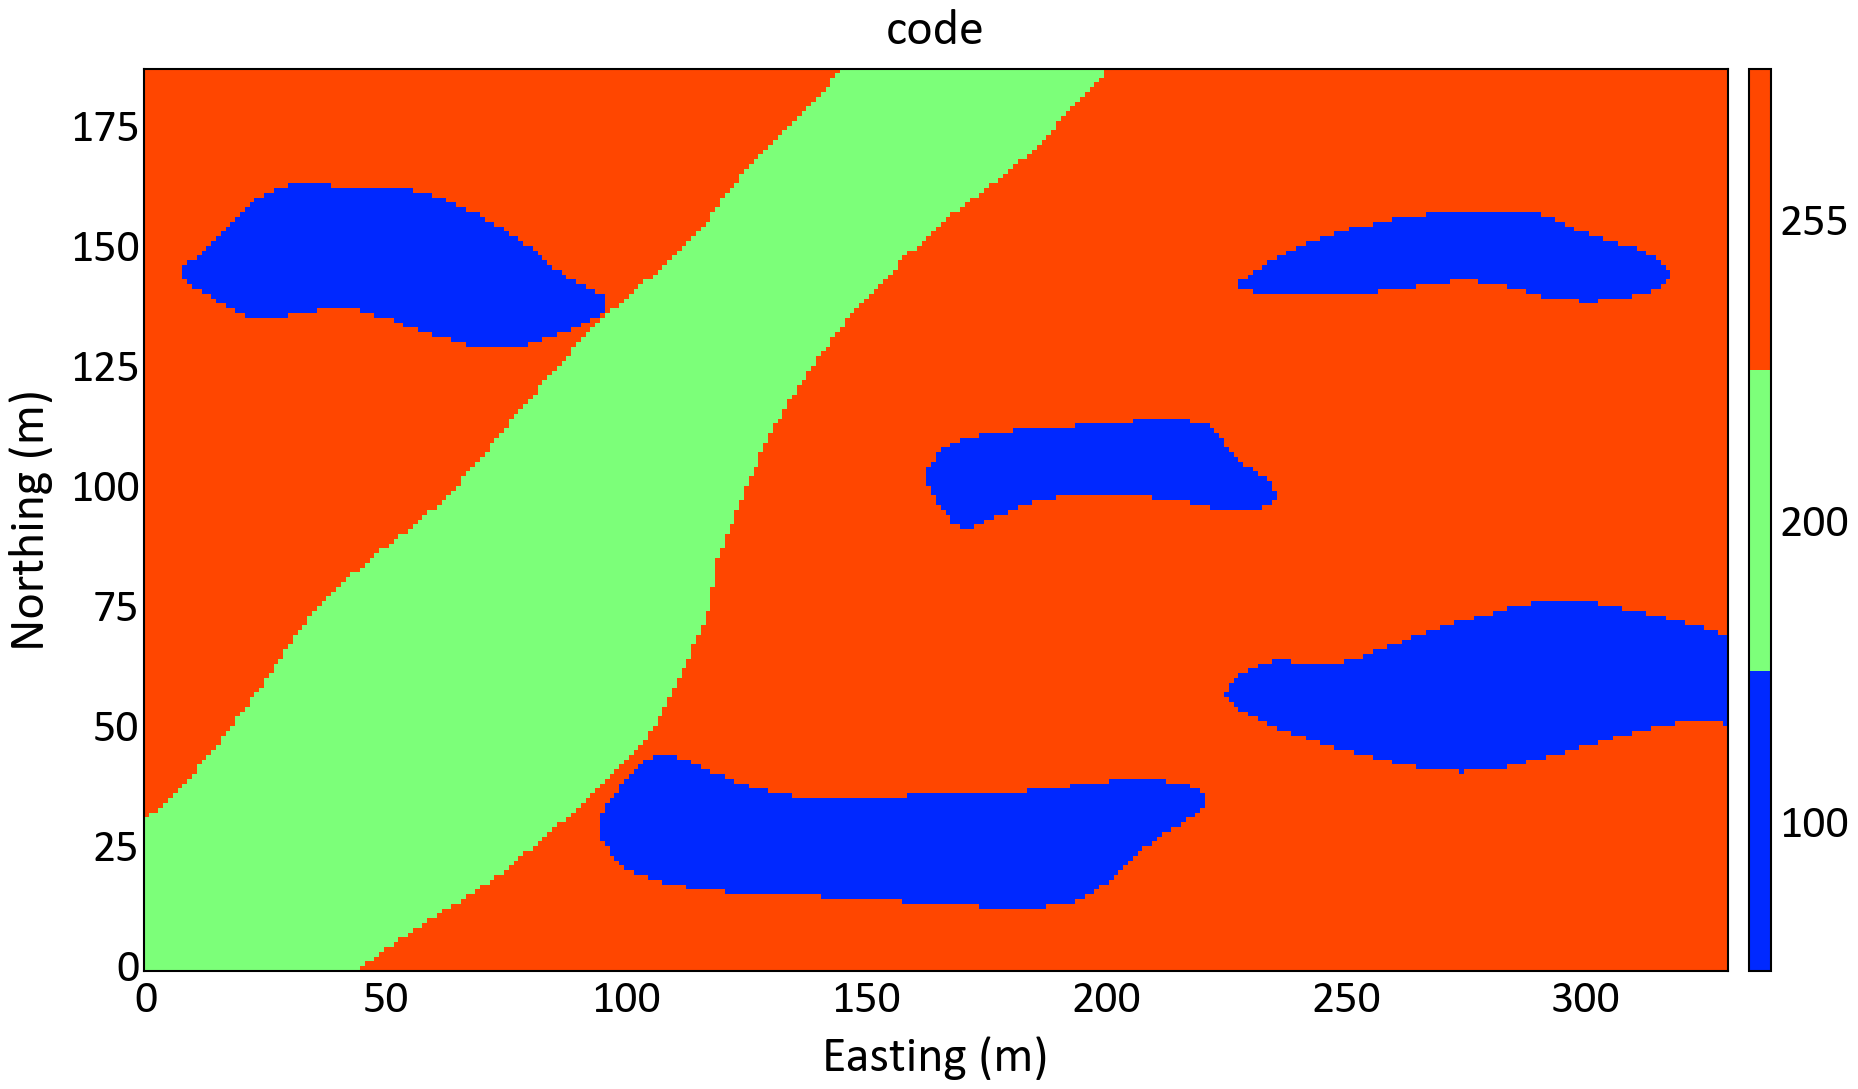
\includegraphics[width=.8\textwidth]{capitulo_3/imagens/exhaustive.png}\label{exa}}
     \\
     \subfloat[][Furos verticais.]{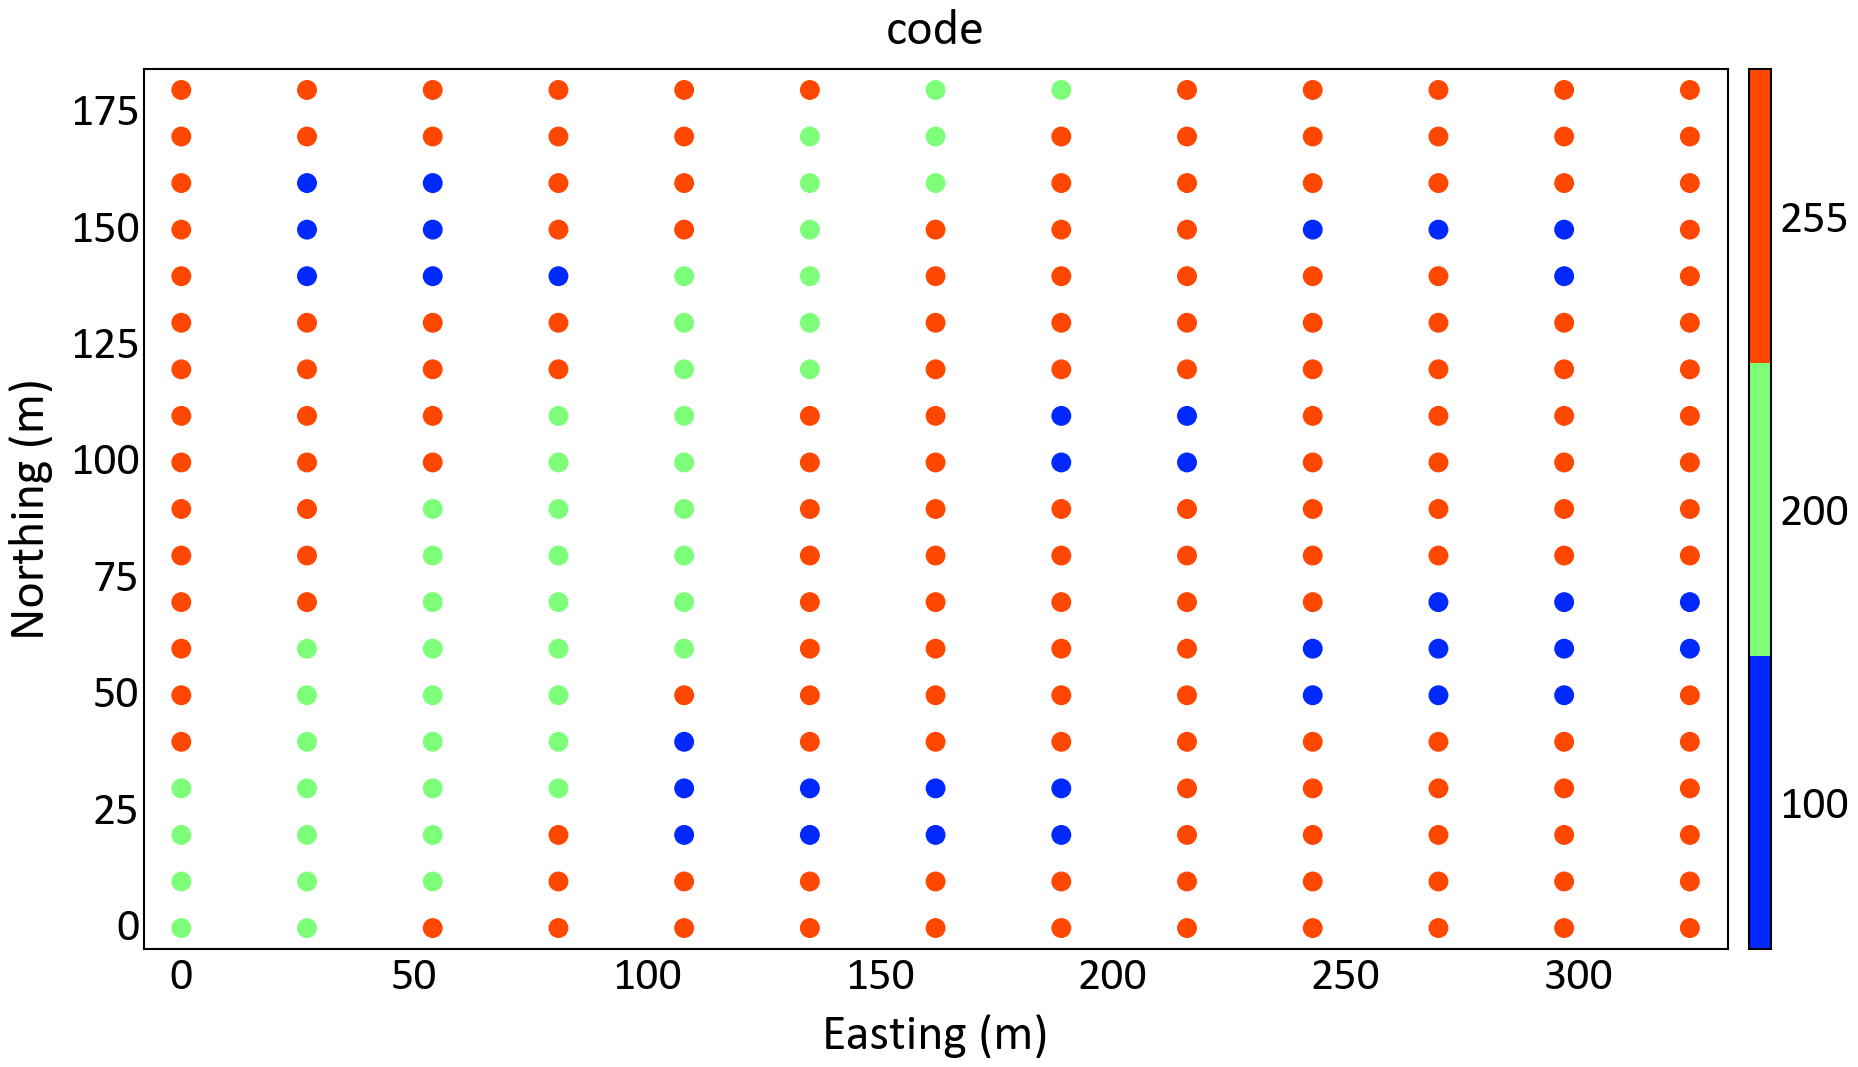
\includegraphics[width=.8\textwidth]{capitulo_3/imagens/sampled_10.png}\label{sampl}}
\end{figure}

O método foi aplicado no banco de dados da Figura \autoref{sampl}. O \textit{grid} de interpolação tem dimensões 1x1 metros. O modelo dos \textit{kernels} é Gaussiano com suportes iguais a 20, 30 e 20 metros para as categorias 255, 200 e 100, respectivamente. Não foi aplicada anisotropia e um efeito pepita de 0.01\% foi utilizado para evitar instabilidades nas matrizes.

Foi utilizada a parametrização linear com fmin otimista=fmin pessimista=0.8 e critério de aceitação de reprodução das amostras igual a 0.85.

A \autoref{synth_reals} mostra duas realizações aprovadas no critério de aceitação de reprodução dos dados amostrais escolhidas aleatoriamente.

Uma animação mostrando todas as 17 realizações (aprovadas no teste de reprodução) pode ser vista \href{https://github.com/robertorolo/kernel_support_parametrization_uncertainty_assess/blob/main/sec_hole_10.gif}{aqui}.

\begin{figure}[H] 
    \centering
    \caption{Realizações para o modelo geológico sintético gearadas a partir dos furos verticais.} \label{synth_reals}
     \subfloat[][Modelo 14.]{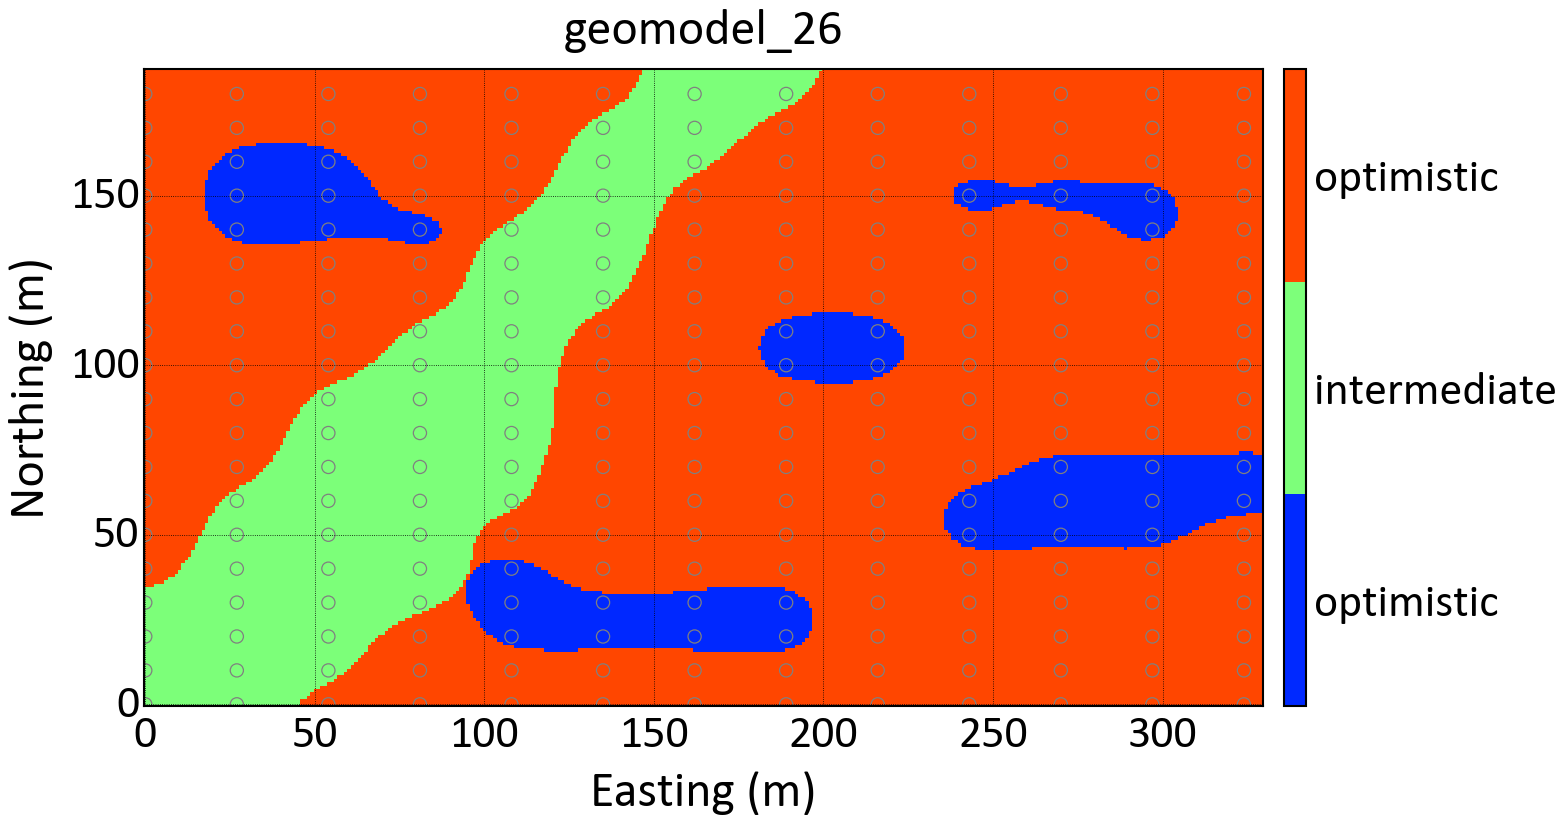
\includegraphics[width=.8\textwidth]{capitulo_3/imagens/sec1.png}\label{mod20}}
     \\
     \subfloat[][Modelo 21.]{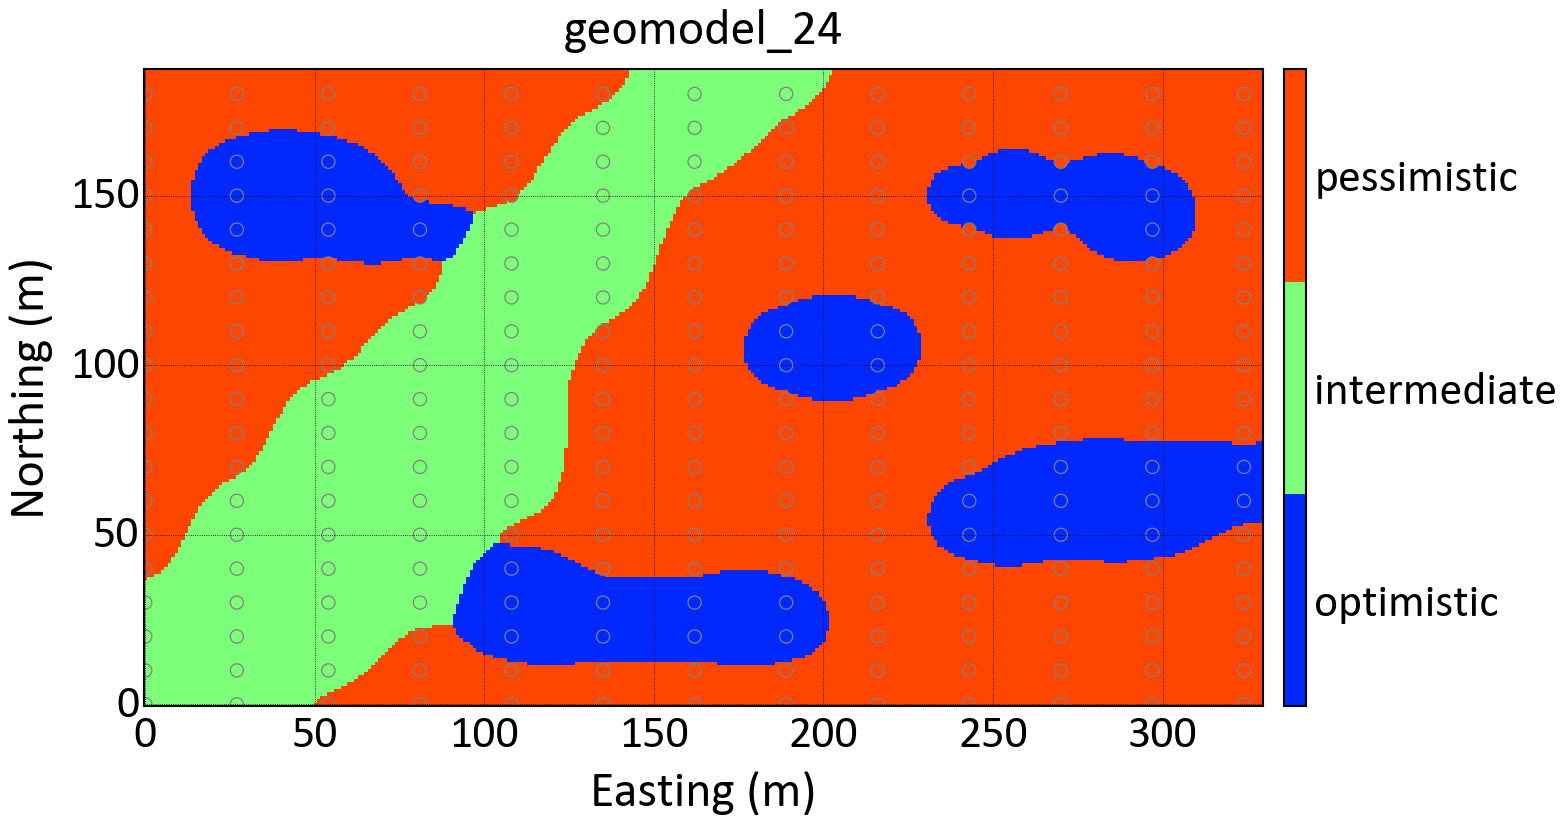
\includegraphics[width=.8\textwidth]{capitulo_3/imagens/sec15.png}\label{mod21}}
\end{figure}

\subsection{Discussão}

O método proposto por \citeonline{mclennanstationarity} é baseado em interpoladores pelo inverso da distância. Por esse motivo, não é possível considerar anisotropia, de forma direta, nos modelos. O autor põe o método em prática apenas em modelos sintéticos de geometria simples, quando aplicado à modelos com geologias complexas a multiplicação dos pesos diretamente pelo fator calculado para cada amostra a partir da parametrização produziu, muitas vezes, volumes (ou áreas) muito grandes ou muito pequenas que não honram os dados amostrais. Aplicar o fator no suporte do \textit{kernel} torna o método menos sensível aos fatores e dá ao usuário um controle maior sobre os modelos gerados, já que é possível diminuir artificialmente o suporte do \textit{kernel} para reduzir sua influência em detrimento da influência da parametrização.

O método proposto, por ser baseado em interpolação global, gera modelos sem ruídos e apresentando o realismo geológico esperado. O método simula diferentes interpretações para cada litologia do modelo geológico contraindo ou inflando os diferentes domínios. 

O usuário pode controlar o quanto os modelos honram os dados amostrais, entretanto, uma maior restrição nesse sentido gera menos cenários diferentes.

Embora a adaptação seja uma melhoria em relação ao método inicialmente proposto ainda existem pontos que precisam de ajustes: as propriedades distância assinaladas interpoladas ainda são, embora menos em relação à implementação original, sensíveis à parametrização. Uma pequena variação no parâmetro fmin gera uma variação muito grande nas propriedades distâncias interpoladas. De modo geral, é necessário reduzir artificialmente o alcance dos variogramas obtidos a partir das amostras. Caso o alcance não seja reduzido a área ou volume dos sólidos é muito grande no caso otimista ou muito pequena no caso pessimista prejudicando a reprodução dos dados amostrais.

A implementação computacional é em Python, o que torna a execução lenta e inviável para estudos de caso tridimensionais com um grande número de amostras e/ou nós de \textit{grid}.

\section{Avaliação de incerteza usando funções distância assinaladas e campos de probabilidades}\label{pfiels_sec}

\citeonline{froidevaux1993probability} propôs uma abordagem para a simulação condicional de variáveis contínuas. Este método dissocia a tarefa de estimar as funções de distribuição de probabilidade local (PDFs) da produção de realizações equiprováveis. A simulação a partir de campos de probabilidade parte da premissa de que as distribuições condicionais locais são conhecidas. As simulações condicionais são então obtidas extraindo realizações desses PDFs locais.

A metodologia proposta se baseia nesse método para simular contatos. A primeira etapa é definir uma largura de banda de incerteza em torno dos contatos entre as diferentes litologias. Como não há incerteza no interior dos domínios, os blocos fora da zona de incerteza são congelados com o valor da categoria responsável pela distância assinalada estimada mais negativa. Simultaneamente, os blocos dentro da zona de incerteza serão classificados como diferentes categorias em diferentes realizações.

A largura da zona de incerteza pode ser definida por um geomodelador com base no tipo de depósito e configuração amostral: em depósitos onde a geologia apresenta variabilidade mais significativa, como depósitos com múltiplas rochas intrusivas por exemplo, ela deve ser mais ampla; em depósitos menos erráticos, como os estratificados, deve ser mais estreita. Em malhas de amostragem com espaçamento próximo, zonas de incerteza menores são necessárias, enquanto em malhas de amostragem esparsas, zonas mais amplas são necessárias.

A distância assinalada estimada em um nó do \textit{grid} é a distância de um bloco ao domínio oposto mais próximo. A zona de incerteza é definida pela retenção de todos os blocos onde o valor absoluto da distância estimada, de pelo menos uma das categorias do banco de dados, é menor ou igual ao valor definido pelo geomodelador para a largura de banda de incerteza.

A estimativa da PDF local é feita transformando as distâncias estimadas em probabilidades em cada um dos blocos da zona de incerteza como mostrado na \autoref{heuristic}.

A partir da modelagem multi-categórica no banco de dados \textit{Swiss Jura} mostrada na \autoref{multicat_jura} foi determinada uma zona de incerteza de 12 metros ao redor dos contatos. Isto é, Para cada uma das distâncias assinaladas interpoladas que representam cada uma das categorias do banco de dados, qualquer bloco em que a distância interpolada pertença ao intervalo [-12,12] é classificado como zona de incerteza.

A \autoref{unc_zone} mostra, do lado esquerdo, blocos definidos como pertencentes à banda de incerteza de 12 metros para o \textit{Swiss Jura}. As cores indicam quantas categorias têm sua distância assinalada interpolada absoluta menor ou igual ao valor da largura de banda (12 metros).

\begin{figure}[H]
	\caption{\label{unc_zone} Da esquerda para a direita: (1) zona de incerteza de 12 metros; (2) distâncias estimadas para um bloco específico; (3) probabilidades transformadas.}
	\centering
		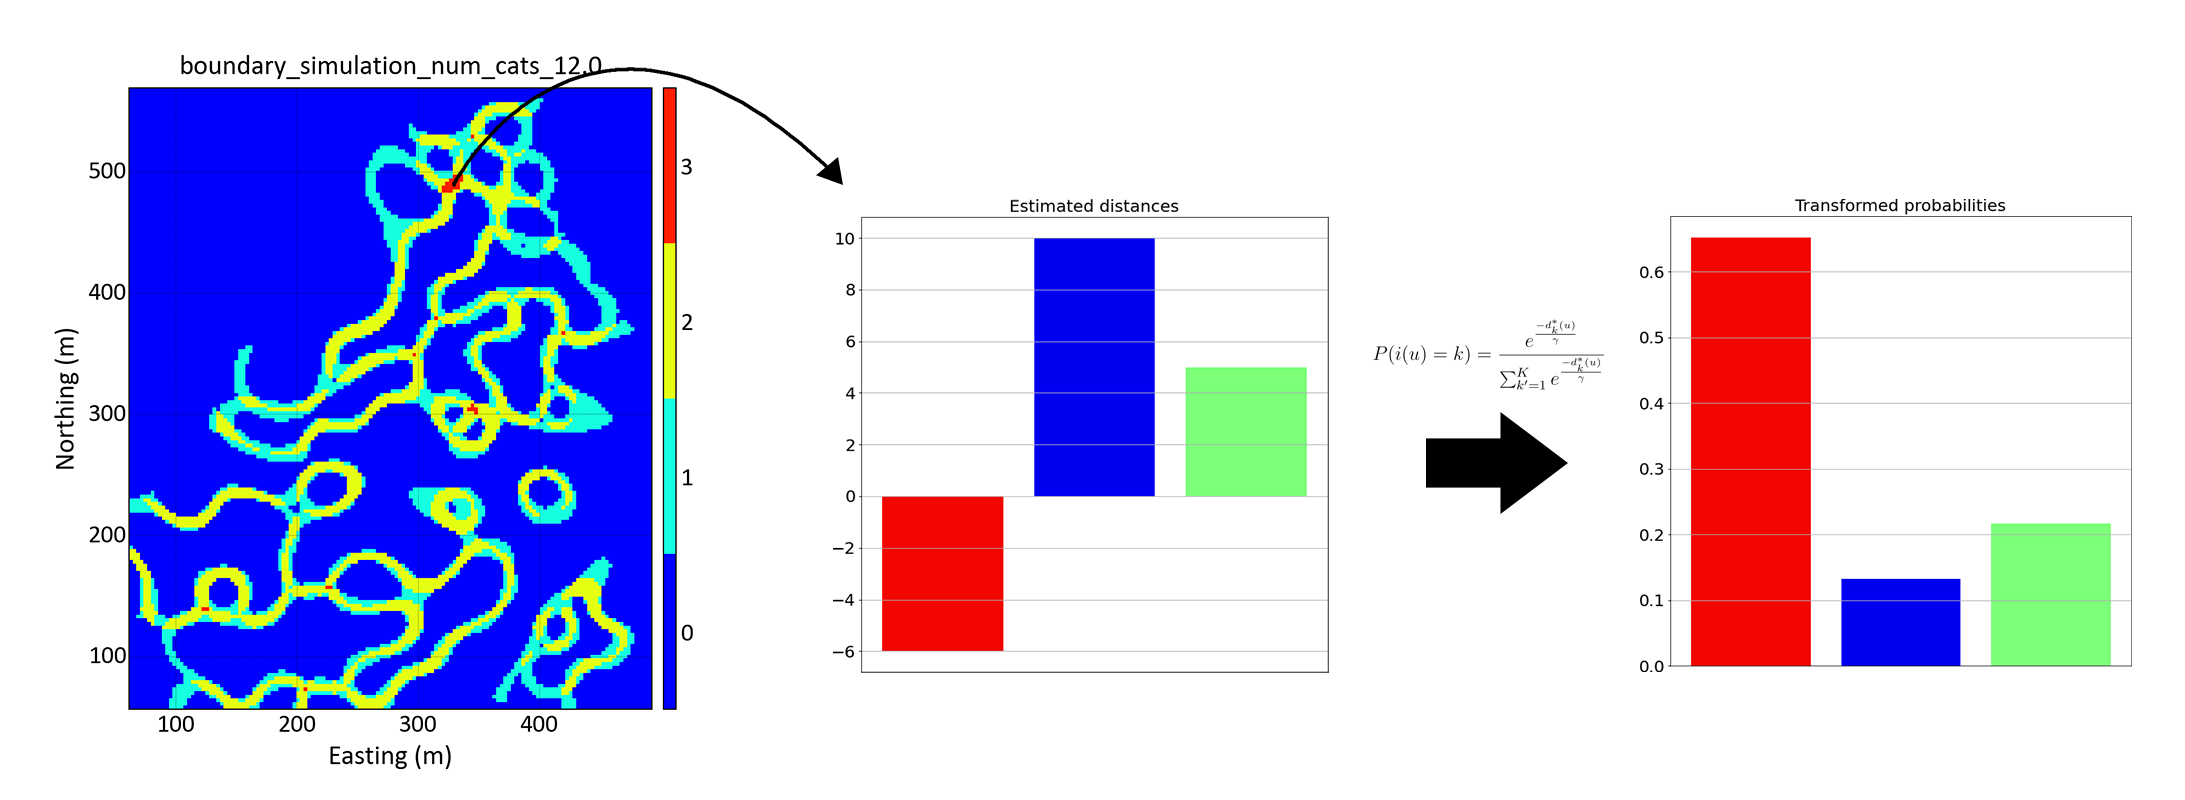
\includegraphics[width=\textwidth]{capitulo_3/imagens/trans_dist_prob.png}
\end{figure}

Observe que, embora haja cinco categorias diferentes no banco de dados, apenas três farão parte da distribuição de probabilidade local em um bloco vermelho; apenas duas em um bloco amarelo e apenas uma em um bloco azul claro. A imagem central mostra as distâncias estimadas para um bloco em específico. Finalmente, no lado direito estão as probabilidades transformadas pela \autoref{eq_softmax} para aquele bloco usando o valor de distância absoluta máxima como o parâmetro $\omega$.

A produção de realizações equiprováveis para o modelo geológico é feita simulando primeiro um campo gaussiano não condicional nos blocos pertencetes à zona de incerteza por simulação sequencial Gaussiana (\autoref{algo:usgs}). Os valores Gaussianos devem ser transformados no campo de probabilidade estandardizando-os para que variem entre 0 e 1 em uma distribuição uniforme. Isso é feito calculando os valores de distribuição Gaussiana cumulativos.

Finalmente, para gerar várias realizações do modelo geológico, uma categoria deve ser amostrada das PDFs locais usando o campo de probabilidade simulado para cada bloco dentro da zona de incerteza em cada realização, como mostrado na \autoref{samplig_from_dist}.

\begin{figure}[H]
	\caption{\label{samplig_from_dist} Um valor de probabilidade simulado de 0,51 é usado para amostrar a categoria vermelha de uma distribuição condicional em um bloco específico.}
	\centering
		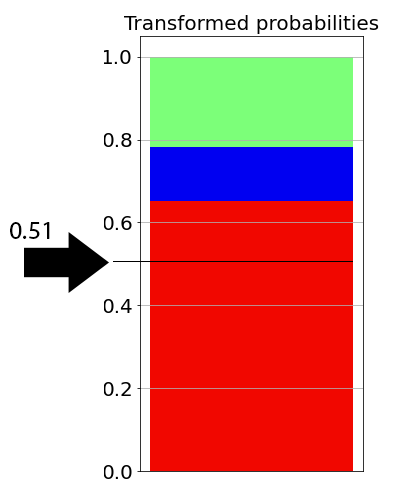
\includegraphics[width=0.3\textwidth]{capitulo_3/imagens/sampling_from_dist.png}
\end{figure}

A \autoref{reals_pfield_jura} mostra, do lado esquerdo, duas realizações diferentes de uma simulação Gaussiana não condicional dentro da zona de incerteza. Ao lado direito, mostra duas realizações do modelo geológico criado pela amostragem de uma categoria das distribuições condicionais locais para o banco de dados \textit{Swiss Jura}. A transição entre as diferentes categorias é suave, pois as simulações Gaussianas têm continuidade espacial. Uma animação mostrando todas as 10 realizações realizadas pode ser vista \href{https://github.com/robertorolo/assessing_geological_model_uncertainty_with_probability_fields/blob/main/jura_gif.gif}{aqui}.

\begin{figure}[H]
	\caption{\label{reals_pfield_jura} Realizações Gaussianas e modelos geológicos correspondentes.}
	 \centering
     \subfloat[][Realização Gaussiana 1]{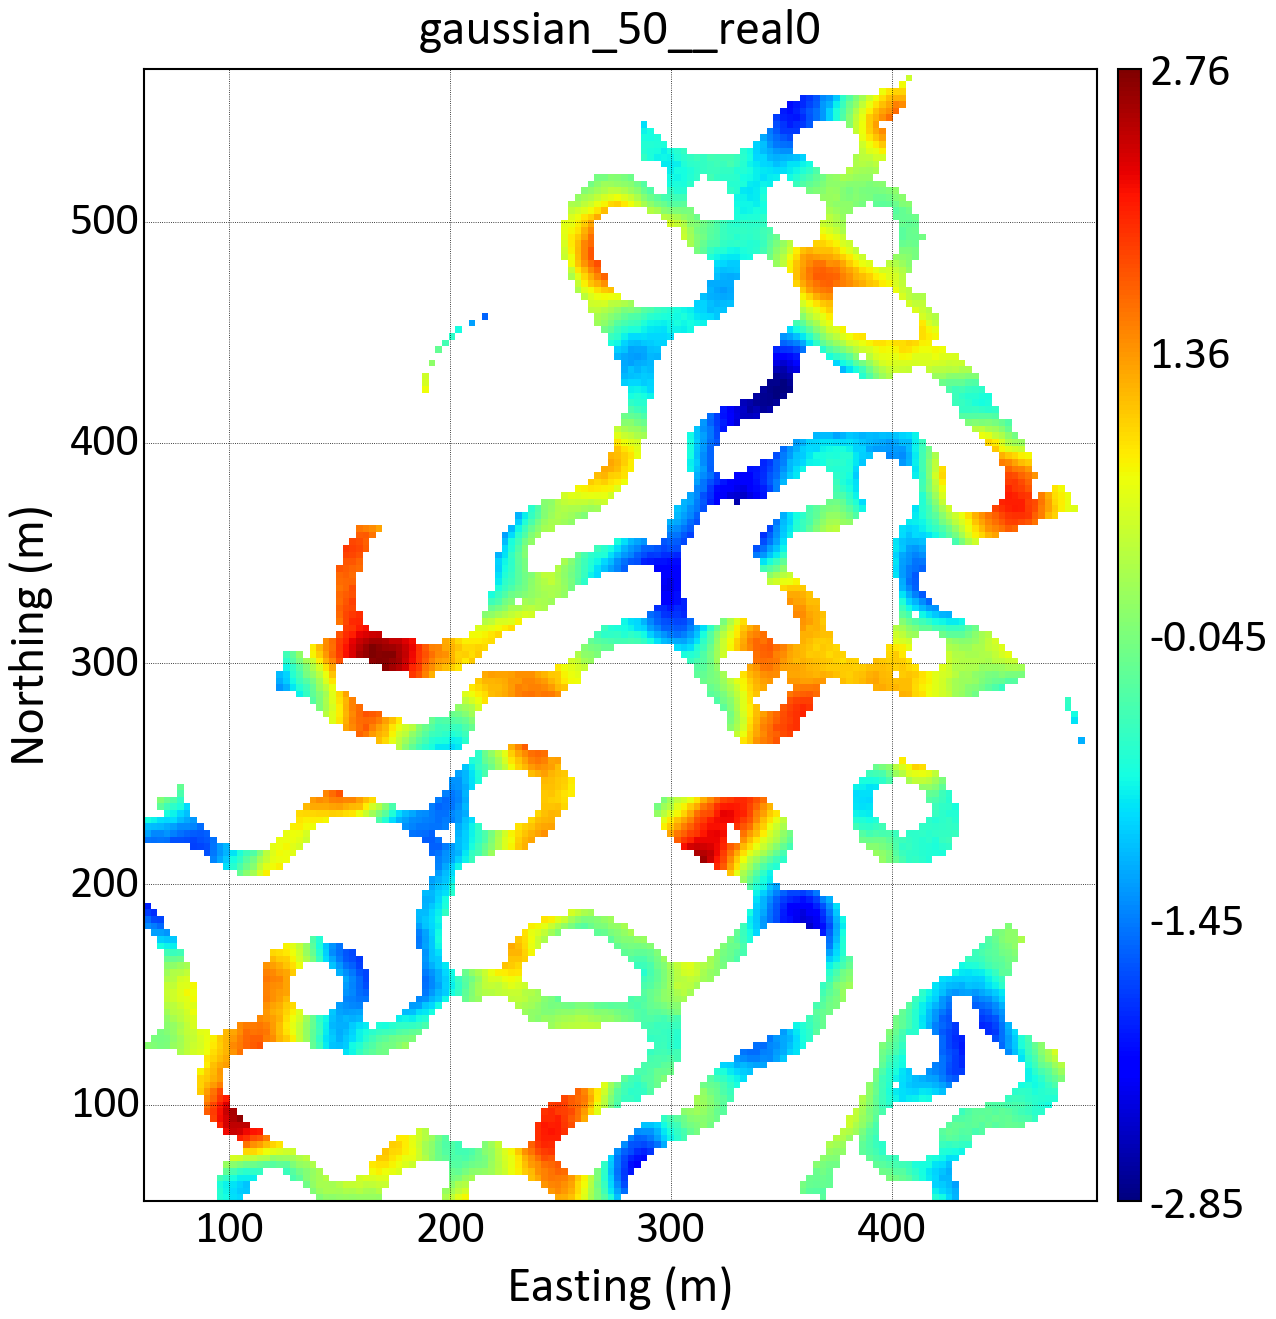
\includegraphics[height=150pt]{capitulo_3/imagens/gausssim_0_12.png}\label{fig:g1}}
     \hspace{1em}
     \subfloat[][Realização do modelo geológico 1]{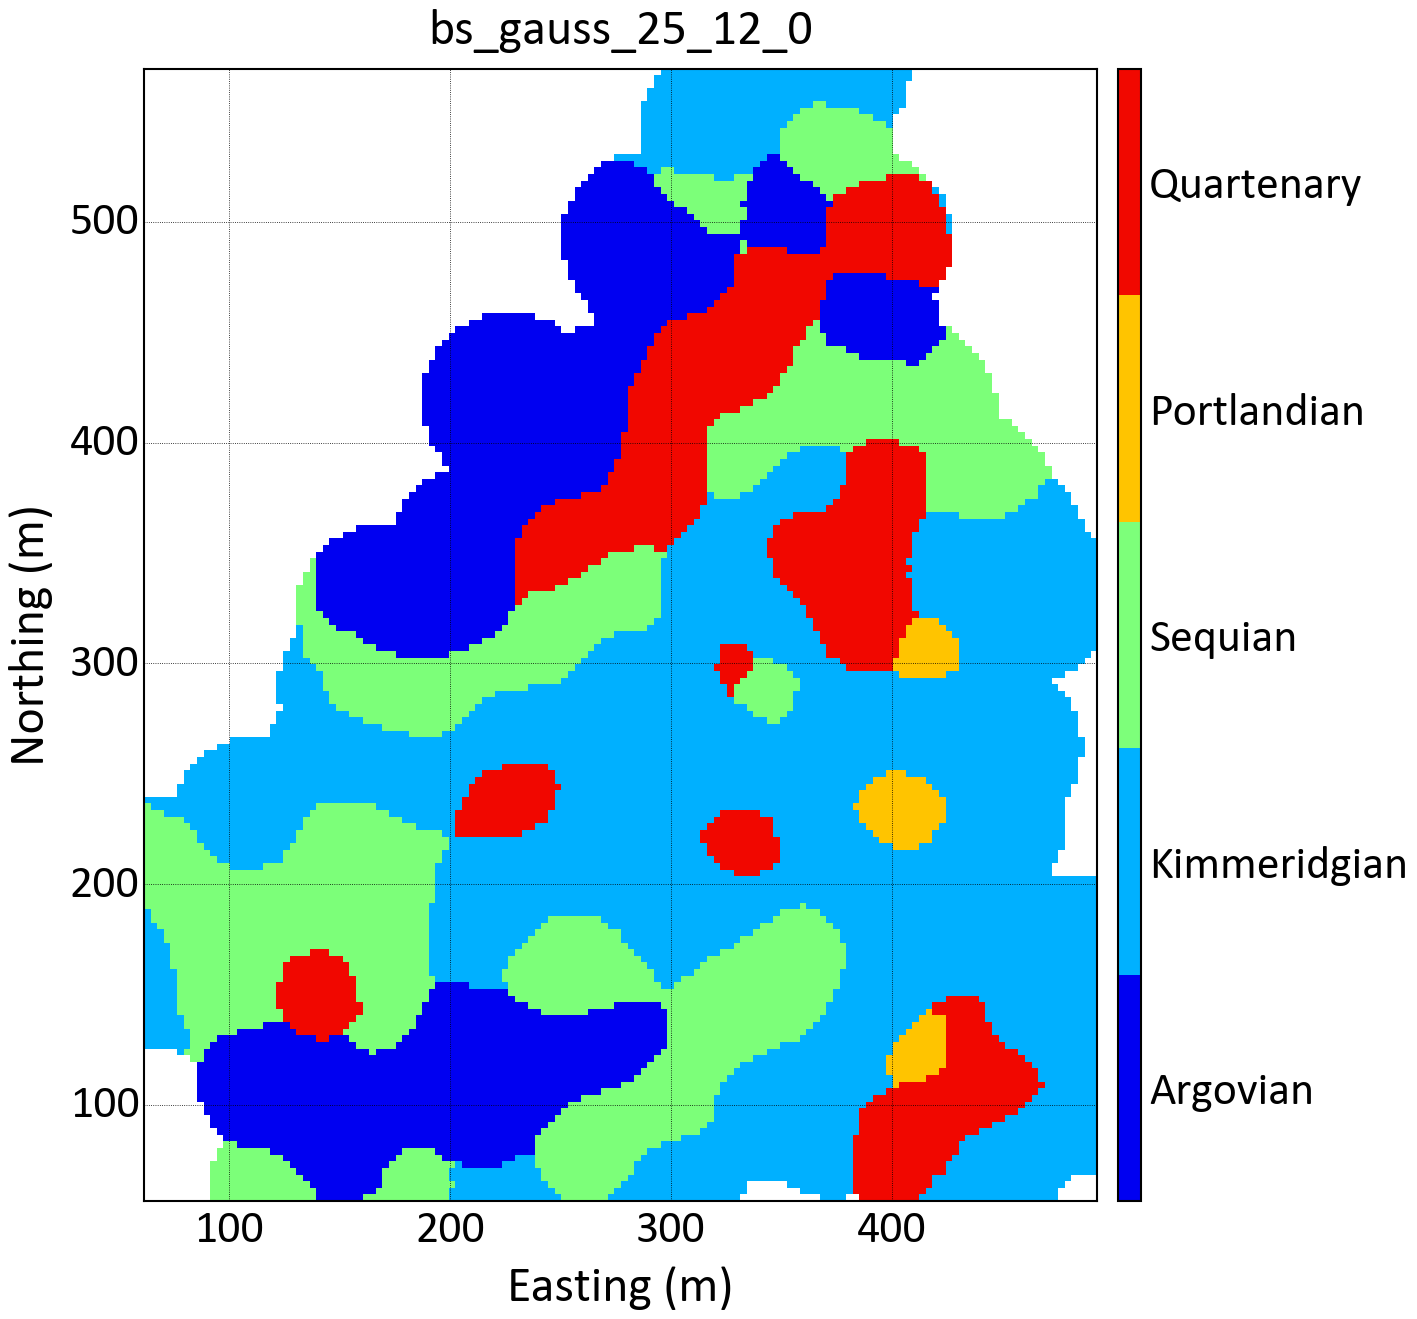
\includegraphics[height=150pt]{capitulo_3/imagens/gauss_real_0_25_12.png}\label{fig:g2}}\\
     \subfloat[][Realização Gaussiana 2]{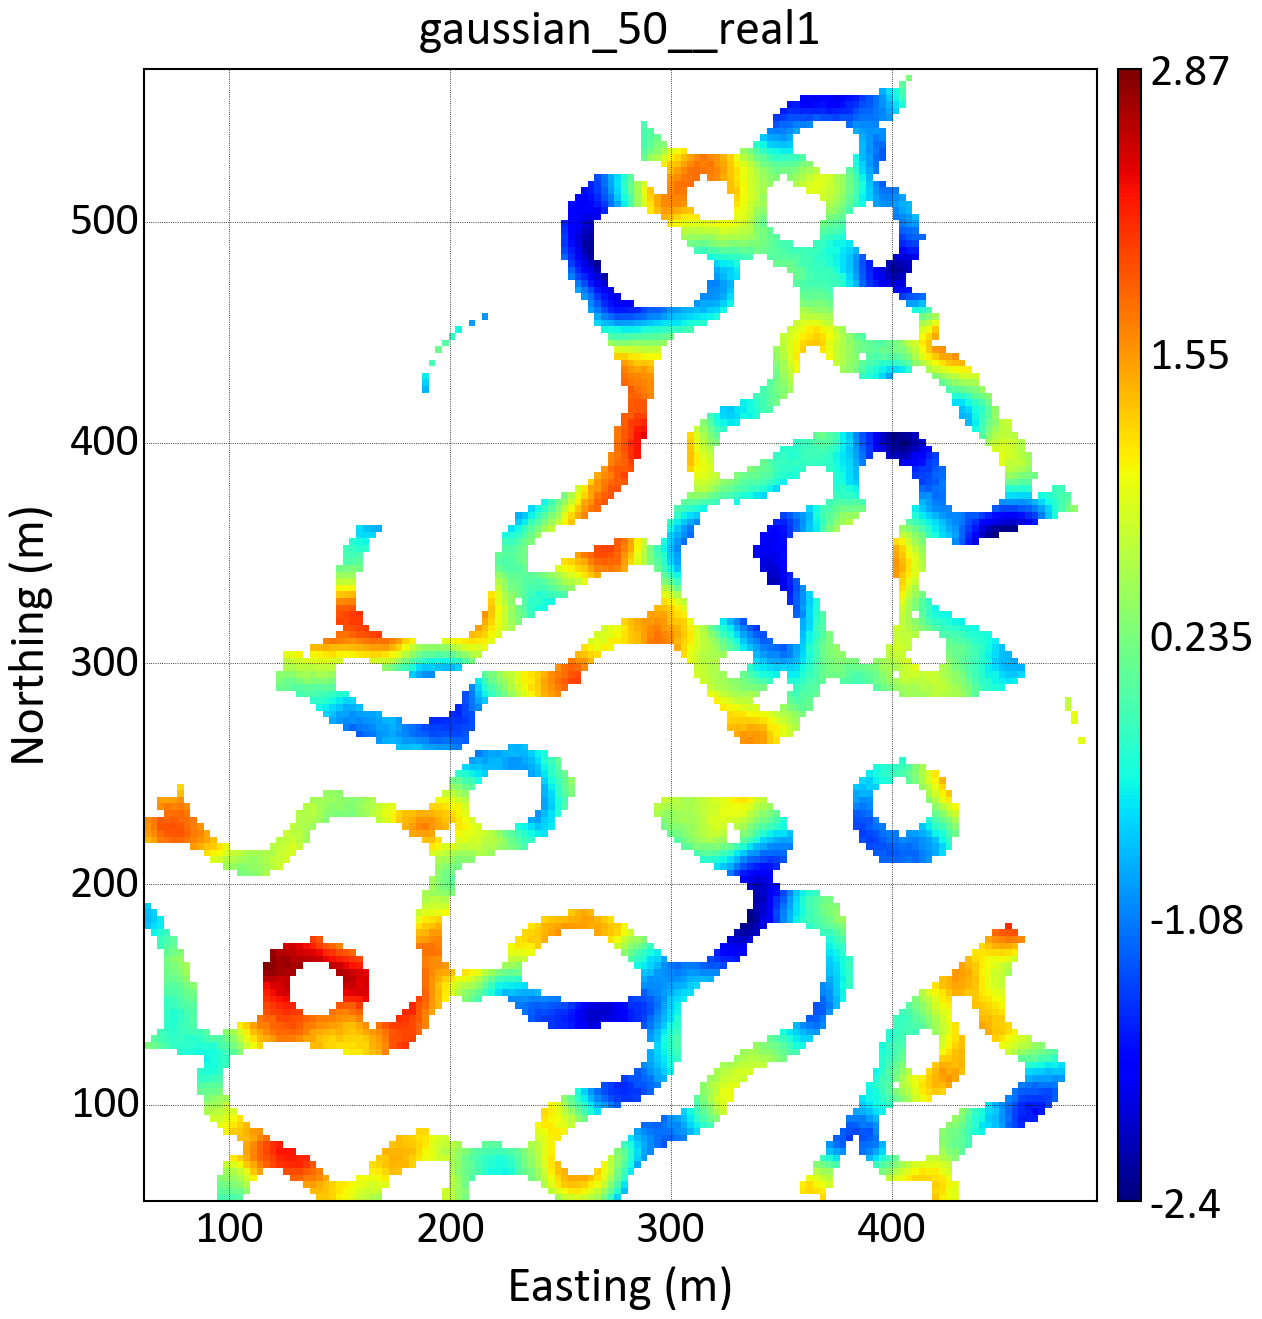
\includegraphics[height=150pt]{capitulo_3/imagens/gausssim_1_12.png}\label{fig:g3}}
     \hspace{1em}
     \subfloat[][Realização do modelo geológico 2]{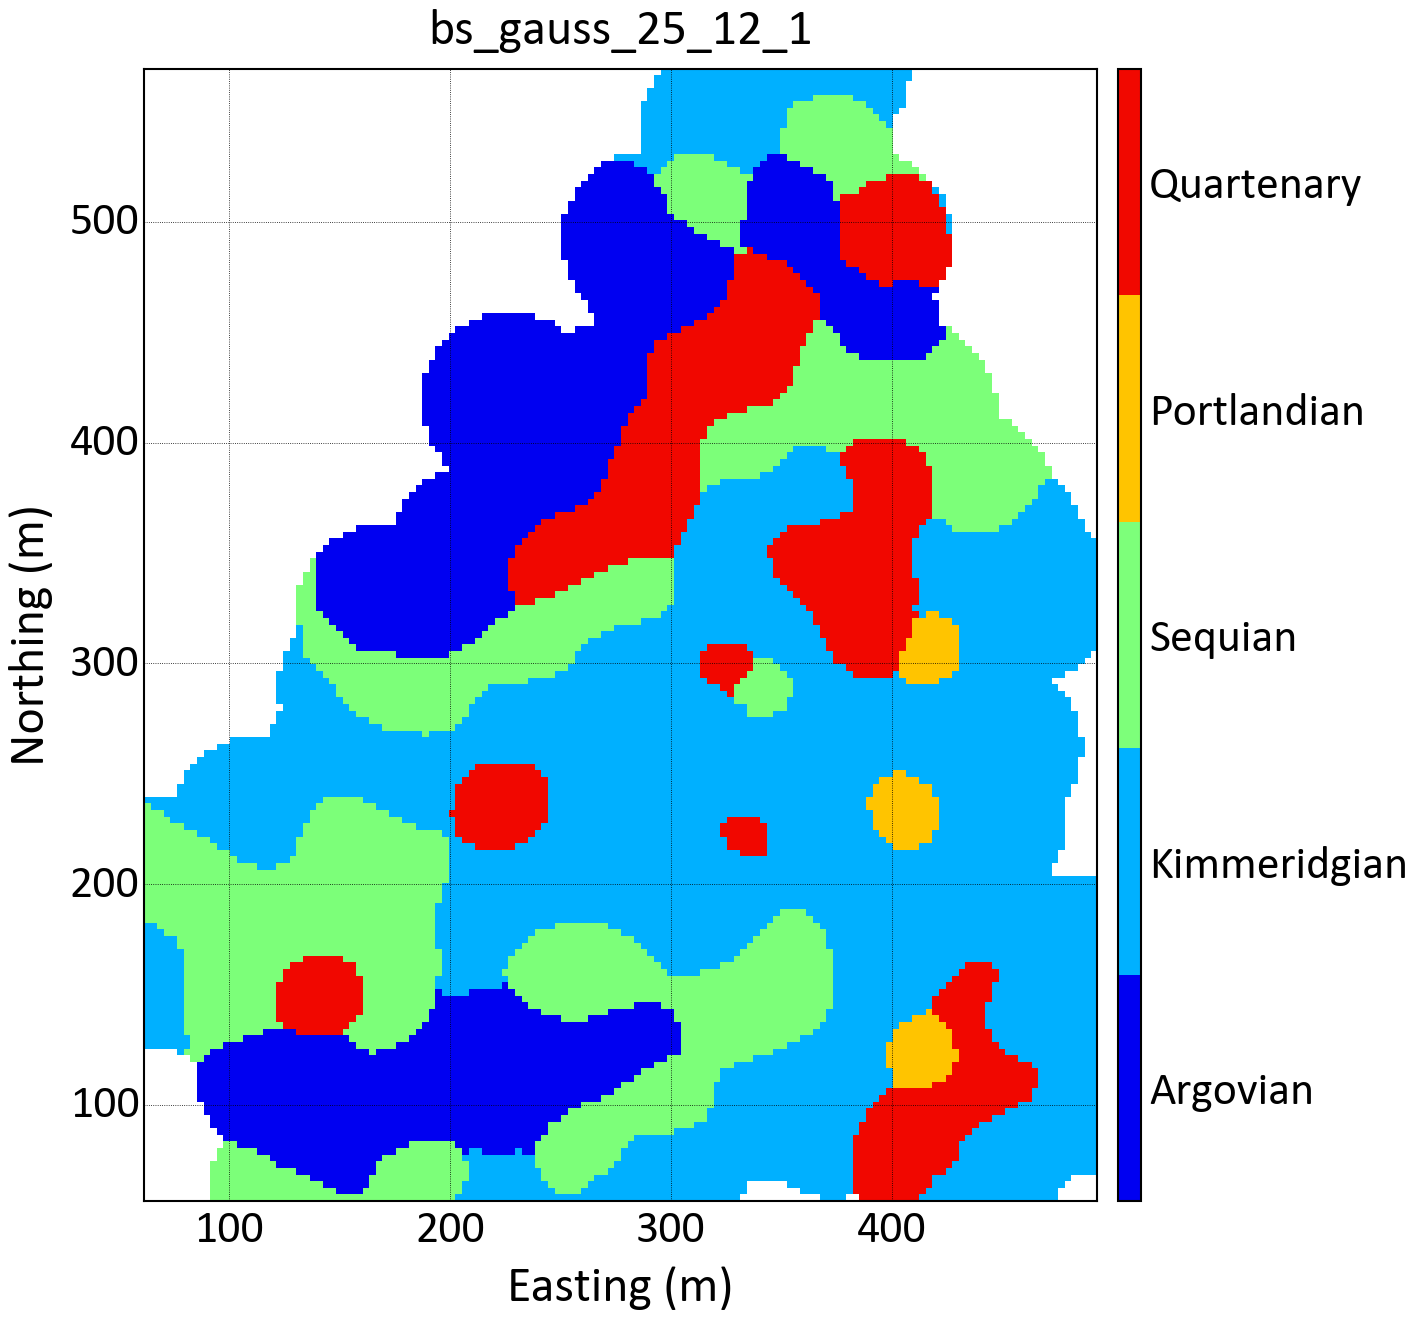
\includegraphics[height=150pt]{capitulo_3/imagens/gauss_real_1_25_12.png}\label{fig:g4}}
\end{figure}

\subsection{Estudo de caso}

Este estudo de caso foi conduzido em um banco de dados real fornecido por uma grande operação de mineração de ouro. O conjunto de dados apresenta 9140 amostras em suporte pontual representando cinco litologias diferentes localizadas em uma área de aproximadamente 10 km² com 1300 metros de profundidade. Uma vista em perspectiva das amostras pode ser vista na \autoref{ouro_amostras}.

\begin{figure}[H]
	\caption{\label{ouro_amostras} Vista em perspectiva das amostras do depósito de ouro.}
	\centering
		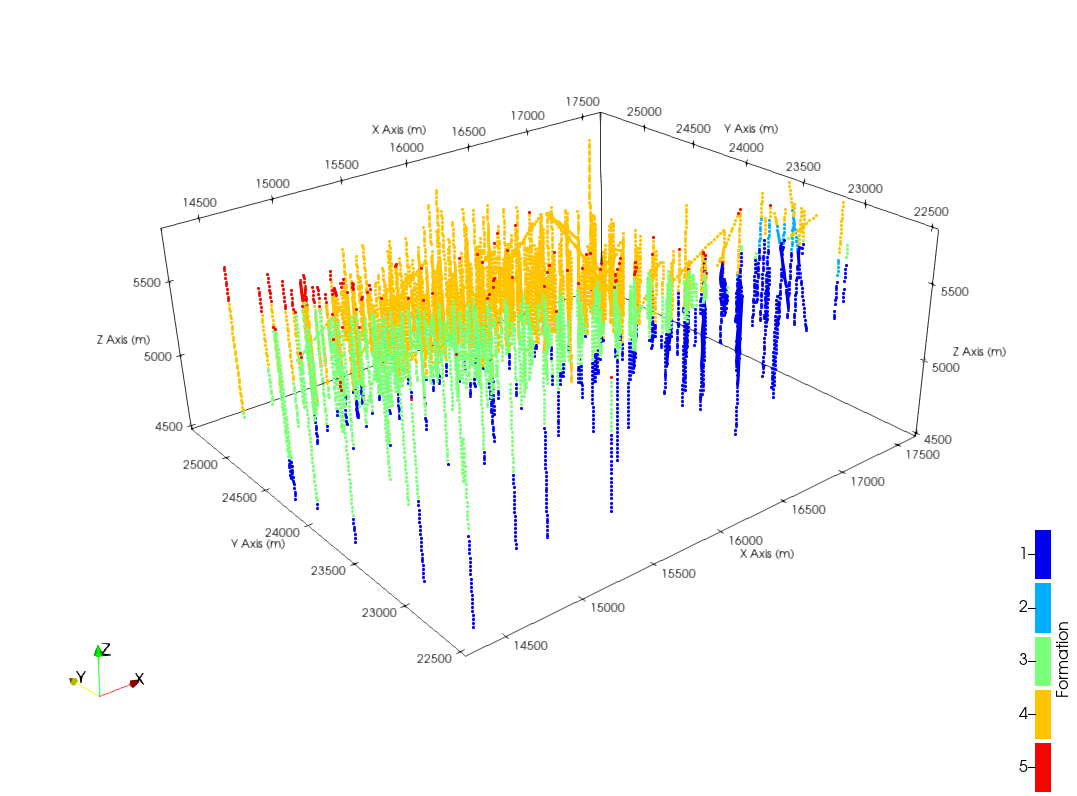
\includegraphics[width=0.8\textwidth]{capitulo_3/imagens/points_perpect.png}
\end{figure}

\citeonline{rolo_dissertacao} e \citeonline{rolo2017signed} realizaram um estudo de caso no mesmo banco de dados, no entanto, os autores utilizaram distâncias assinaladas para criar um modelo geológico multi-categórico determinístico. O presente trabalho é uma extensão natural do trabalho acima mencionado, uma vez que é simples e direto avaliar a incerteza do modelo geológico usando campos de probabilidade a partir das distâncias estimadas usadas para modelagem geológica determinística.

Os variogramas dos indicadores para as cinco categorias do depósito de ouro foram calculados e modelados com estruturas esféricas, conforme mostrado na \autoref{ouro_vargs}. Para os grupos 2, 3, 4 e 5, um variograma omnidirecional foi calculado e modelado. Já para a categoria 1, foram calculados e modelados variogramas omni-horizontal (em azul) e vertical (em vermelho).

\begin{figure}[H]
    \caption{Variogramas dos indicadores para todas as cinco categorias do depósito mineral modelados com estruturas esféricas.} \label{ouro_vargs}
     \centering
     \subfloat[][Variograma omni-horizontal em azul e vertical em vermelho para a categoria 1.]{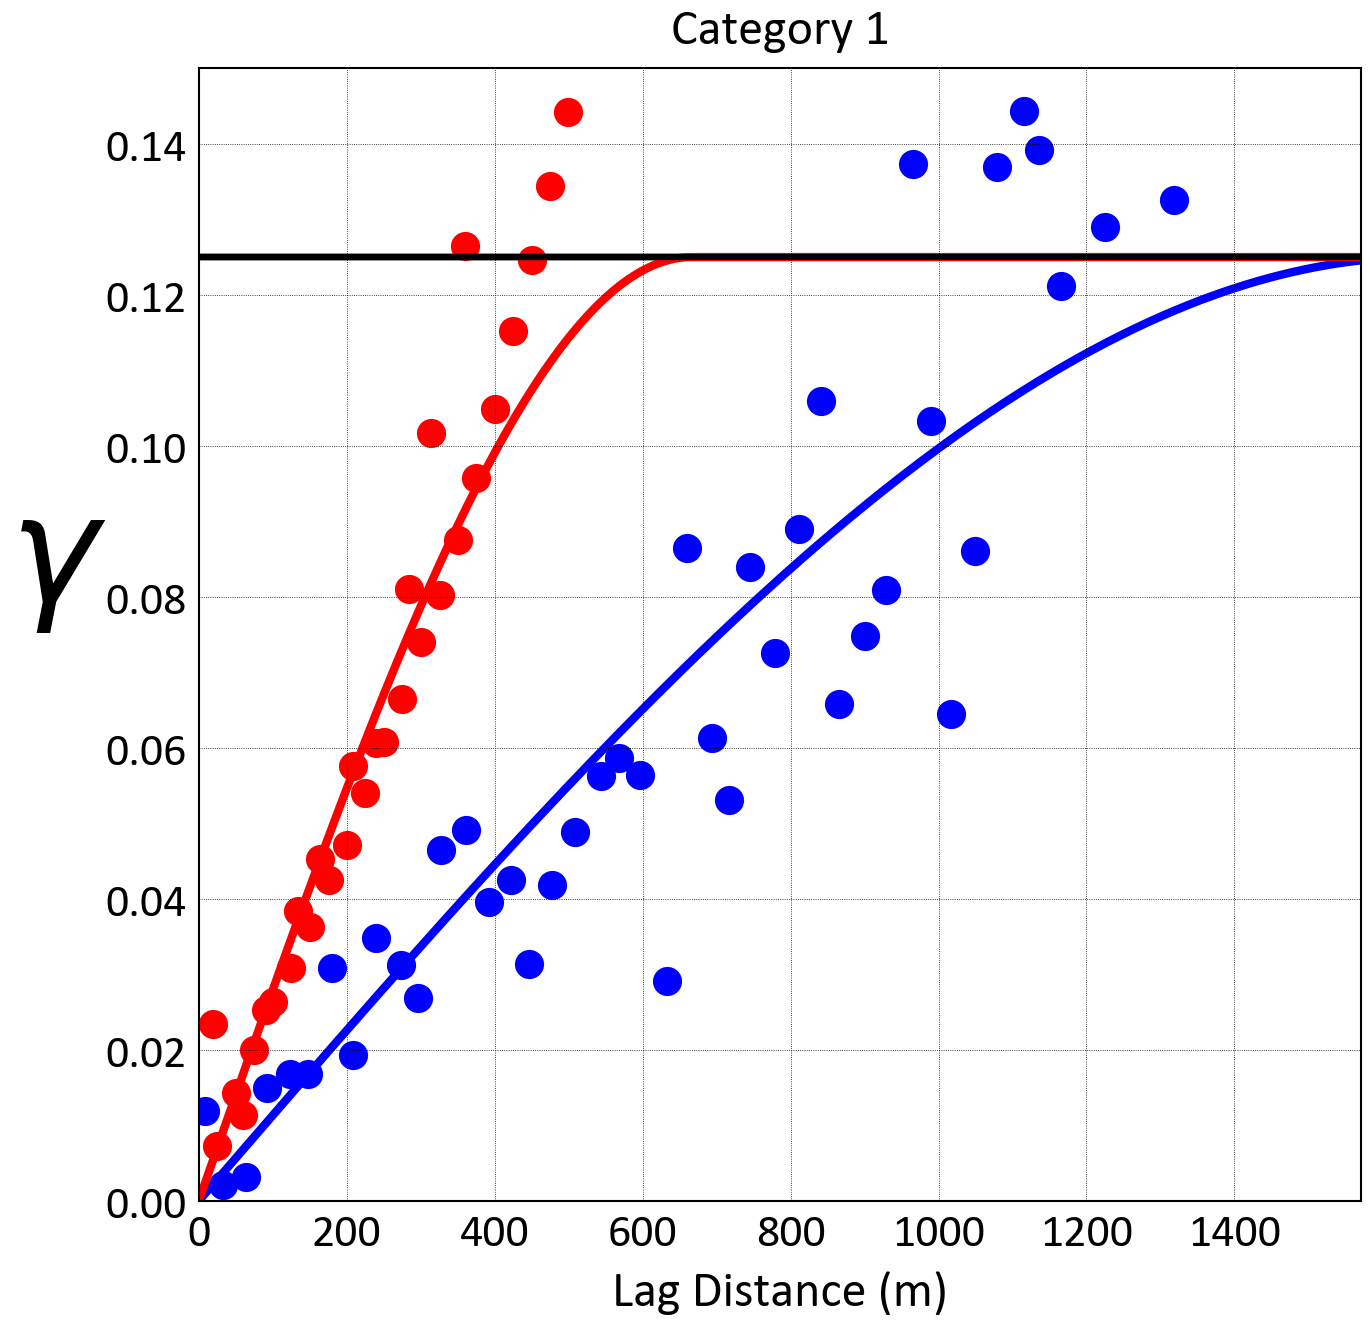
\includegraphics[height=150pt]{capitulo_3/imagens/var_1.png}\label{fig:v1}}
     \hspace{1em}
     \subfloat[][Variograma omnidirecional para a categoria 2.]{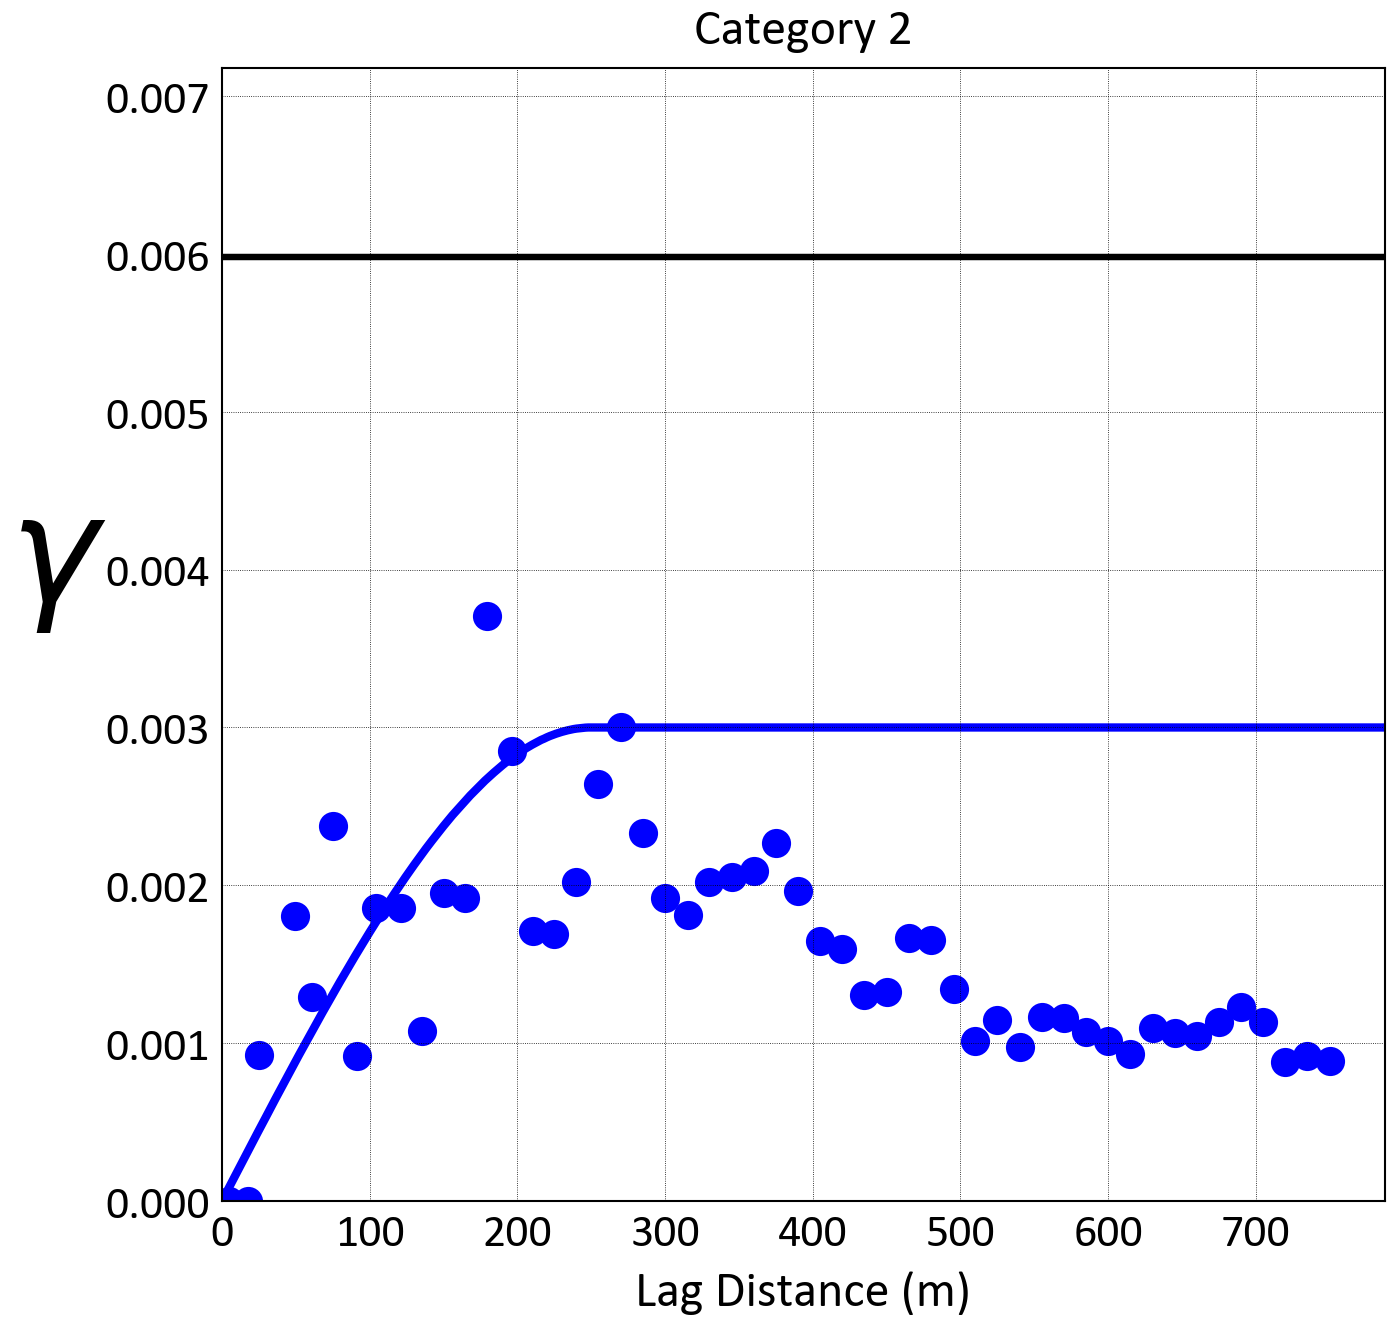
\includegraphics[height=150pt]{capitulo_3/imagens/var_2.png}\label{fig:v2}}\\
    \subfloat[][Variograma omnidirecional para a categoria 3.]{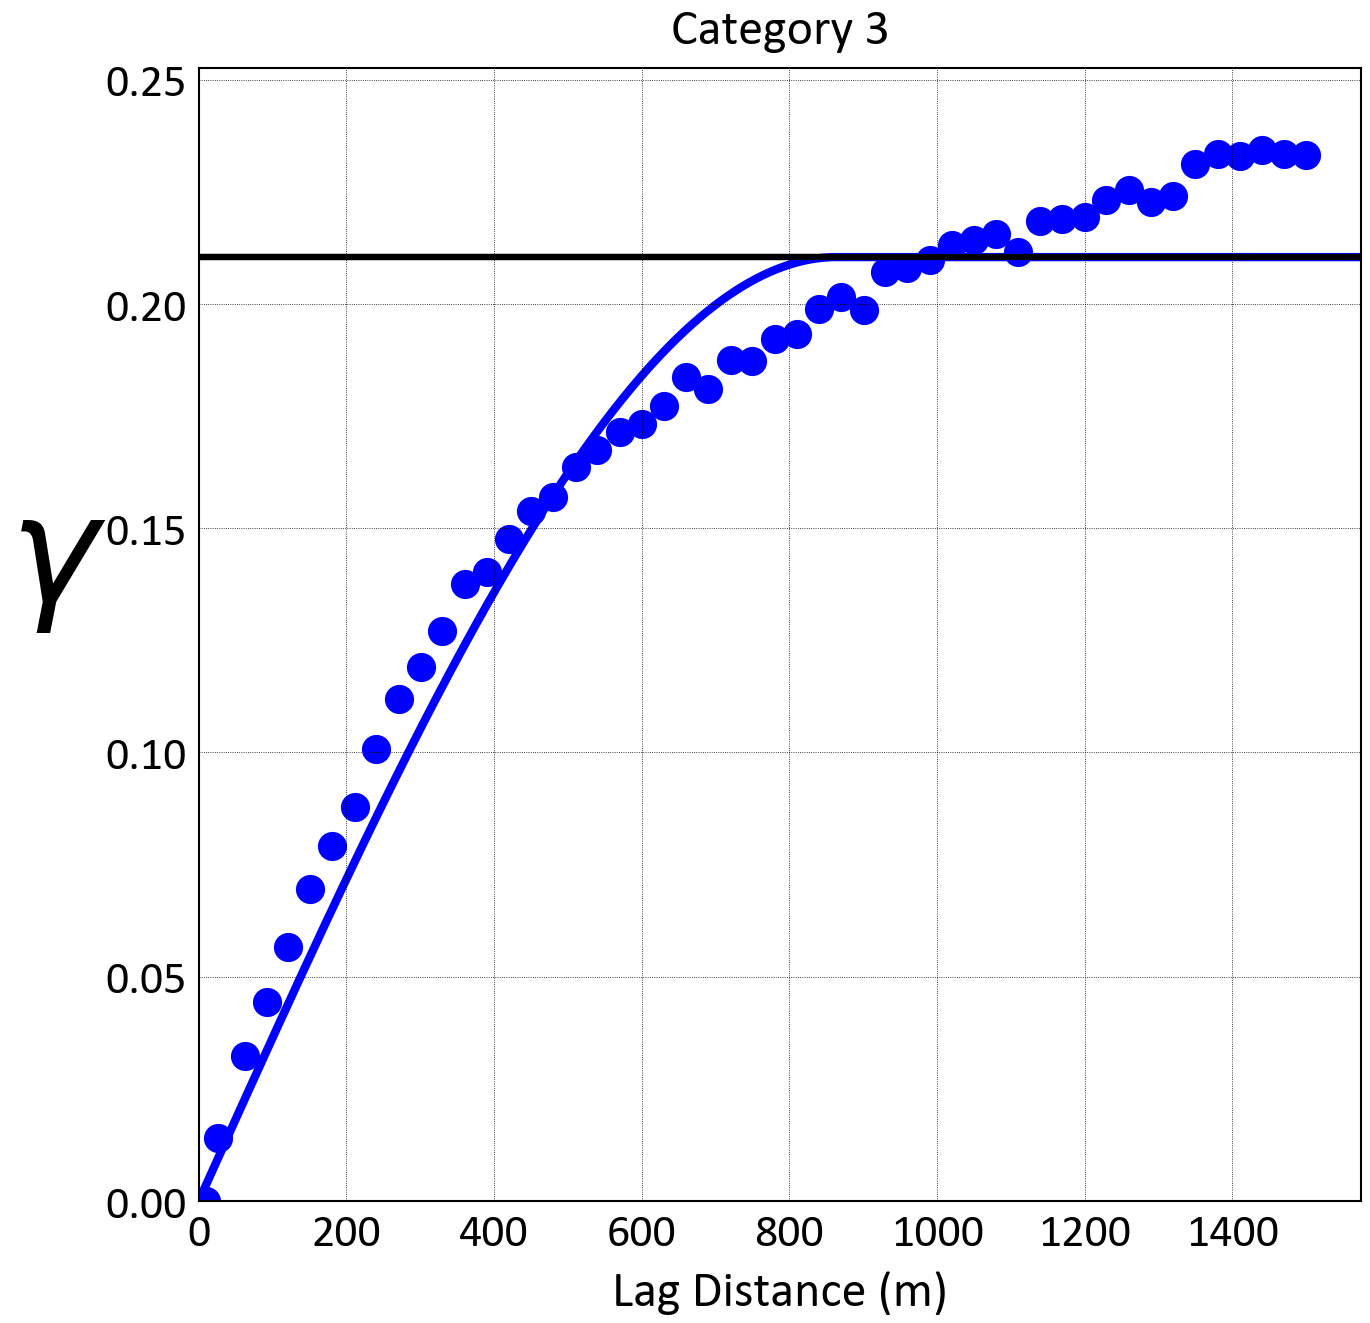
\includegraphics[height=150pt]{capitulo_3/imagens/var_3.png}\label{fig:v3}}
    \hspace{1em}
    \subfloat[][Variograma omnidirecional para a categoria 4.]{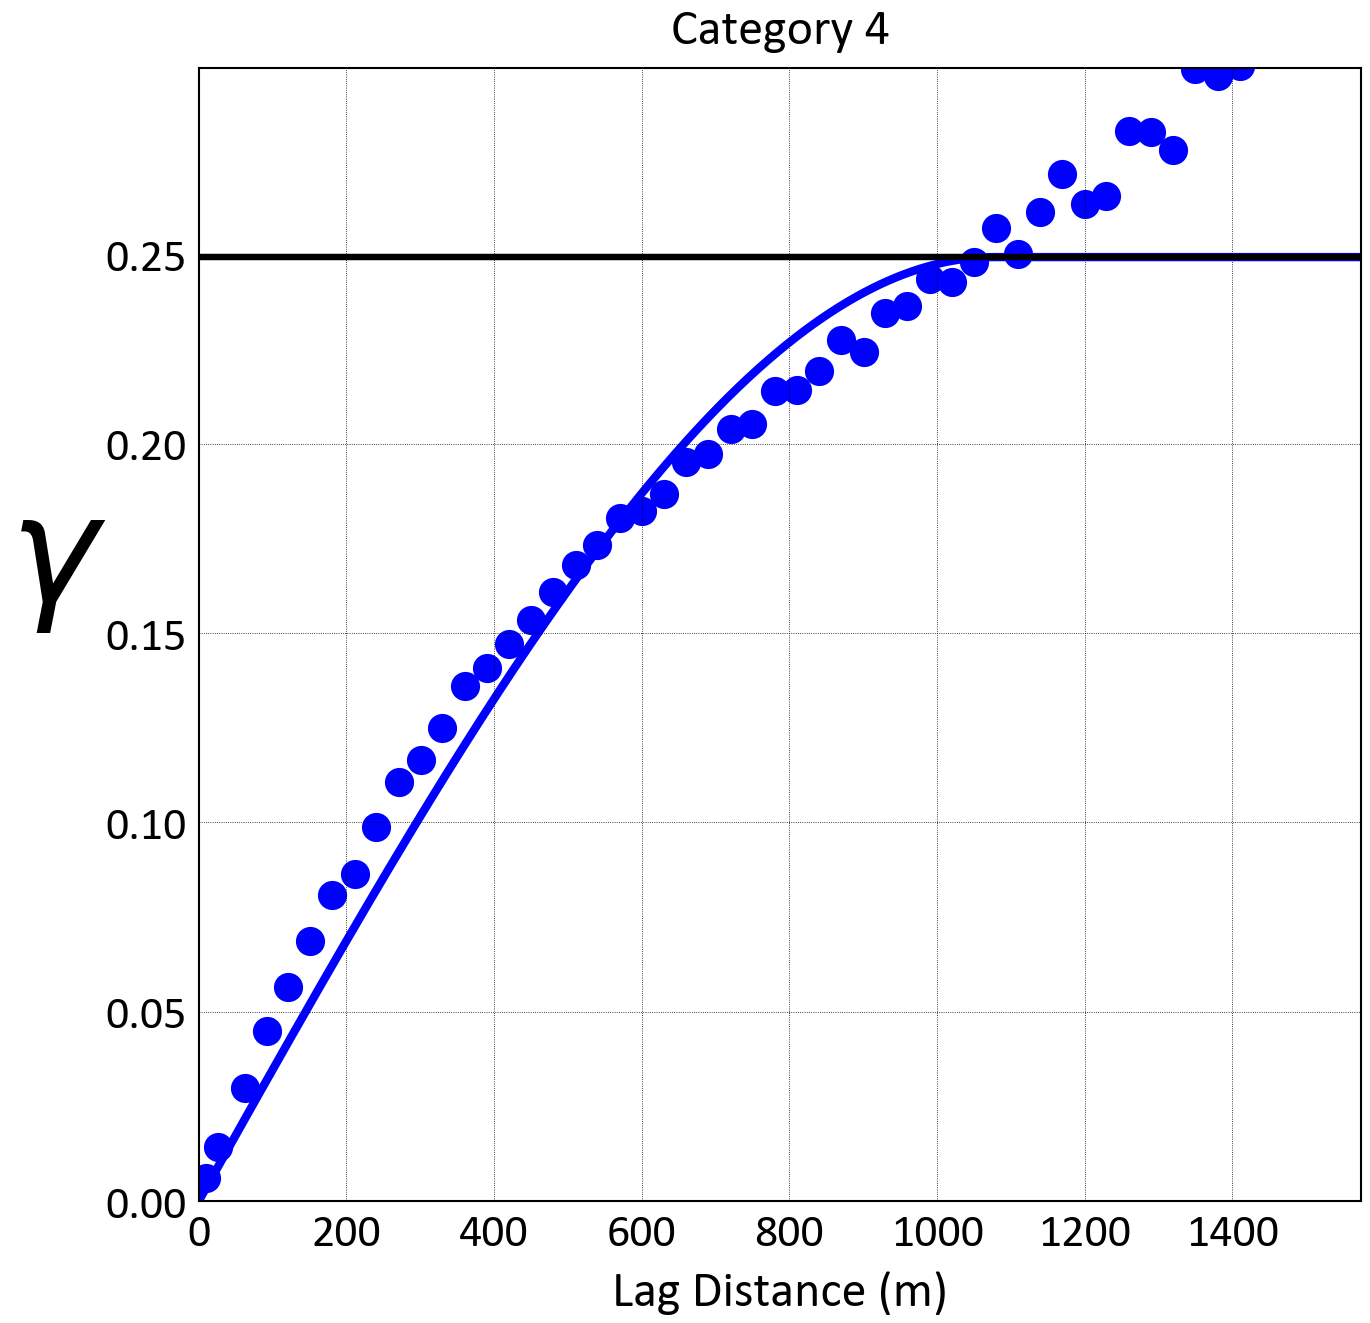
\includegraphics[height=150pt]{capitulo_3/imagens/var_4.png}\label{fig:v4}} \\
    \subfloat[][Variograma omnidirecional para a categoria 5.]{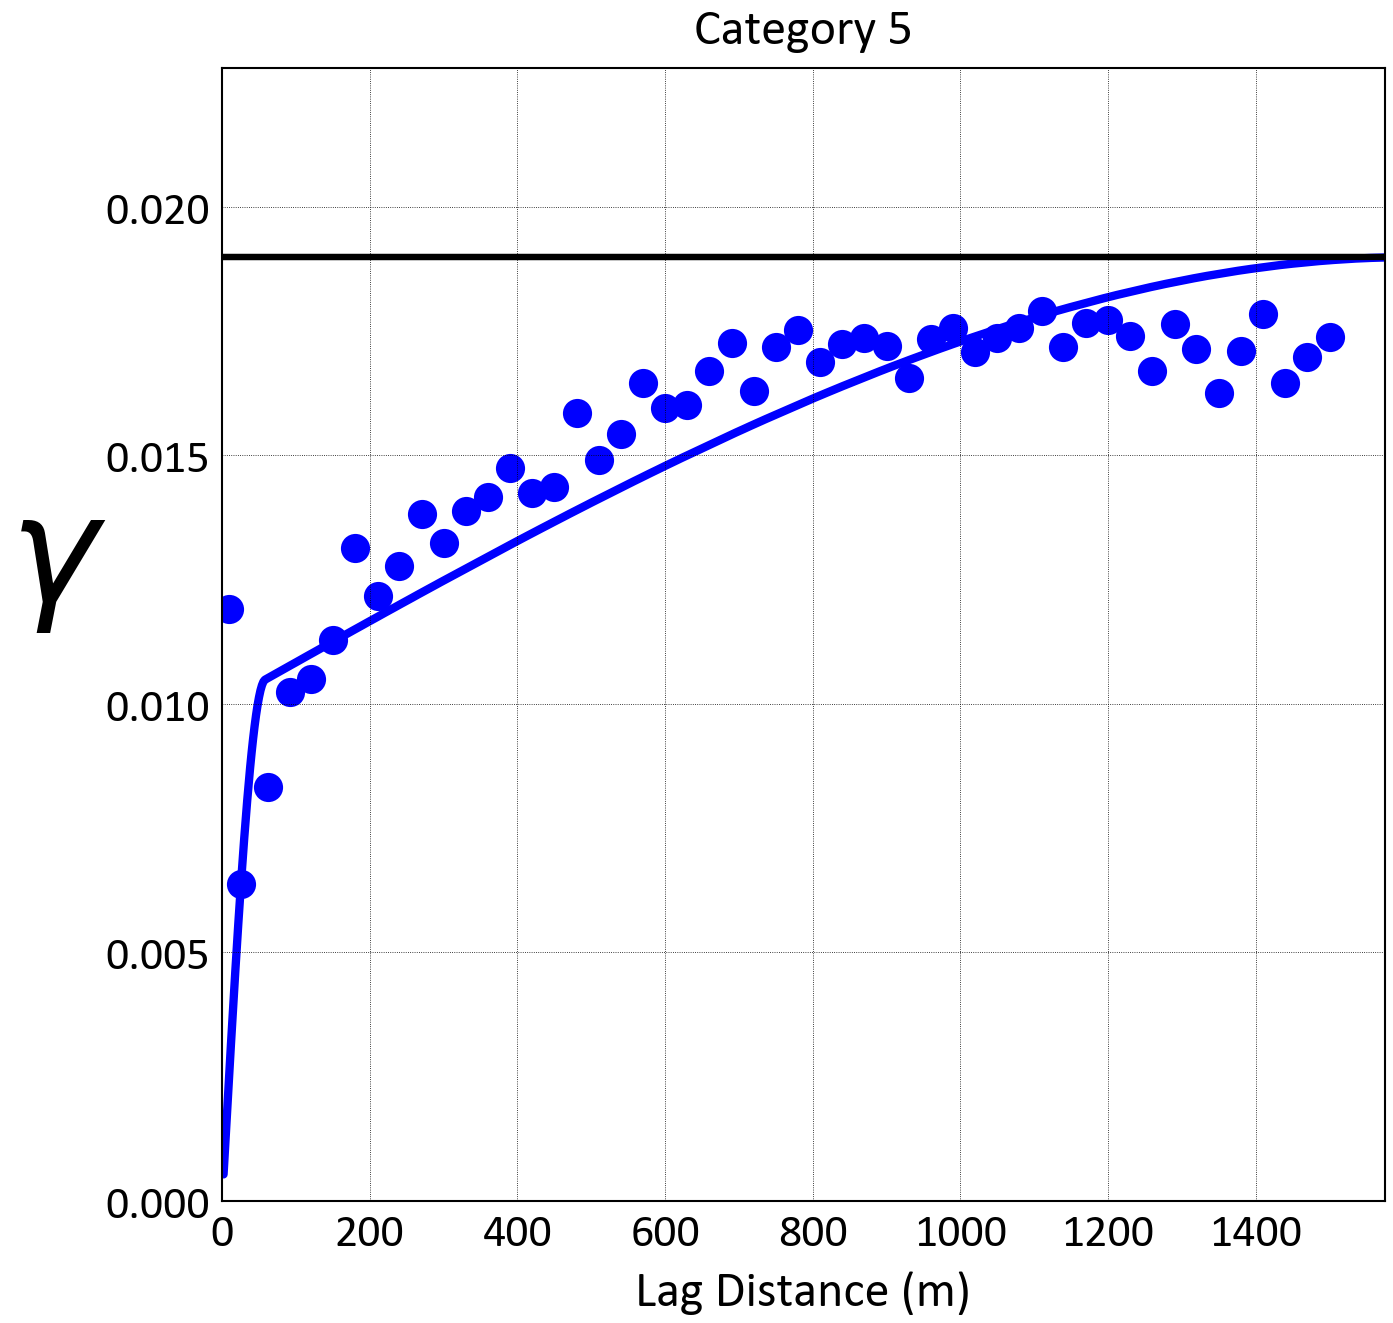
\includegraphics[height=150pt]{capitulo_3/imagens/var_5.png}\label{fig:v5}}
\end{figure}

As distâncias assinaladas calculadas foram interpoladas, por krigagem dual, para um \textit{grid} de 50x50x25 metros usando um equivalente Gaussiano para os variogramas dos indicadores ajustados com modelos esféricos (mesmas contribuições, alcances e razões de anisotropia). Essas dimensões foram escolhidas para o \textit{grid} porque a interpolação dos teores de ouro e posterior planejamento mineiro são feitos, também, nesse \textit{grid}.

Uma largura de 80 metros foi escolhida para a zona de incerteza com base no tipo de depósito e na configuração geométrica amostral. Blocos fora da zona de incerteza foram classificados com a categoria responsável pela distância estimada mais negativas, enquanto blocos dentro da zona de incerteza foram simulados.

Dez realizações de uma simulação não condicional Gaussiana foram realizadas, dentro da zona de incerteza, usando um variograma Gaussiano com um alcance de 600 metros e um pequeno (0,01\%) efeito pepita para evitar instabilidades matemáticas. As realizações foram transformadas em campos de probabilidade e usadas para amostrar uma categoria das distribuições de probabilidade locais. As probabilidades locais foram calculadas transformando as distâncias estimadas, dentro da zona de incerteza, em probabilidades. A distância máxima estimada absoluta foi usada como o parâmetro $\omega$ para cada bloco, dessa forma, a magnitude da incerteza foi controlada apenas pela largura de zona de incerteza. A \autoref{ouro_reals} mostra uma vista em perspectiva de seções verticais e horizontais de duas das 10 realizações para o modelo geológico juntamente com as amostras em suporte pontual.

\begin{figure}[H]
	\caption{\label{ouro_reals} Visão em perspectiva de seções verticais e horizontais de duas realizações do modelo geológico juntamente com as amostras em suporte pontual.}
	\centering
		\subfloat[][Realização 1]{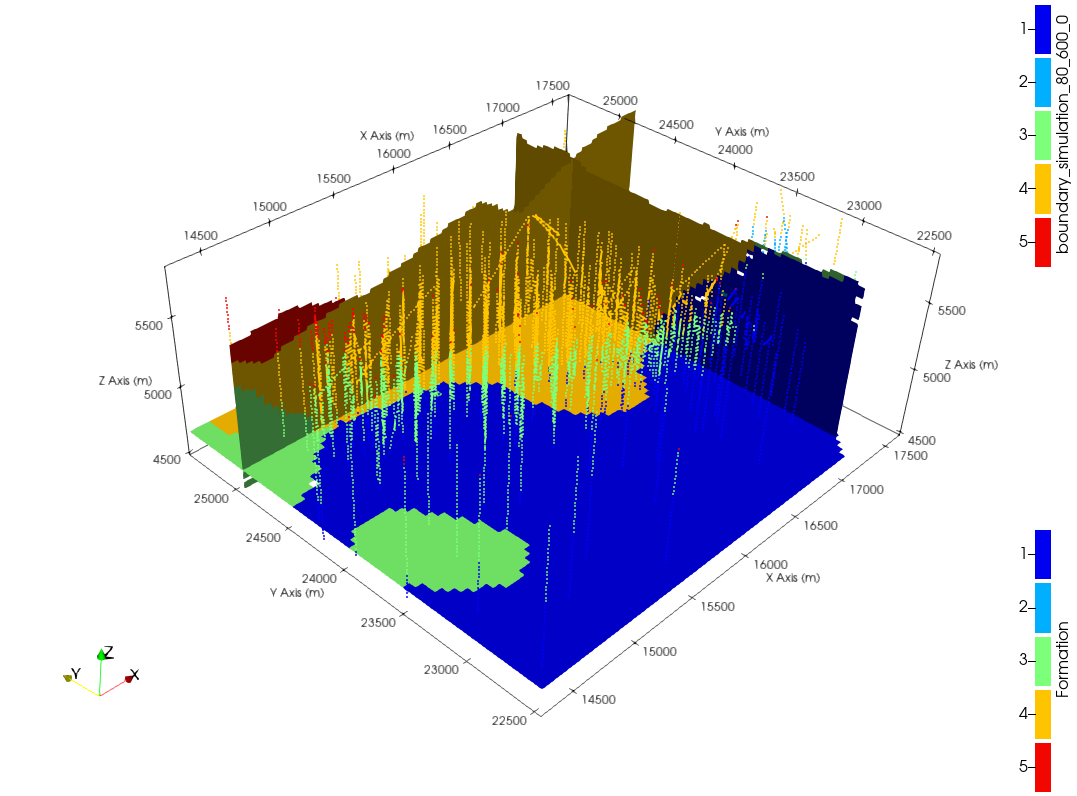
\includegraphics[width=0.45\textwidth]{capitulo_3/imagens/real1.png}\label{fig:g1}}
     \hspace{1em}
     \subfloat[][Realização 2]{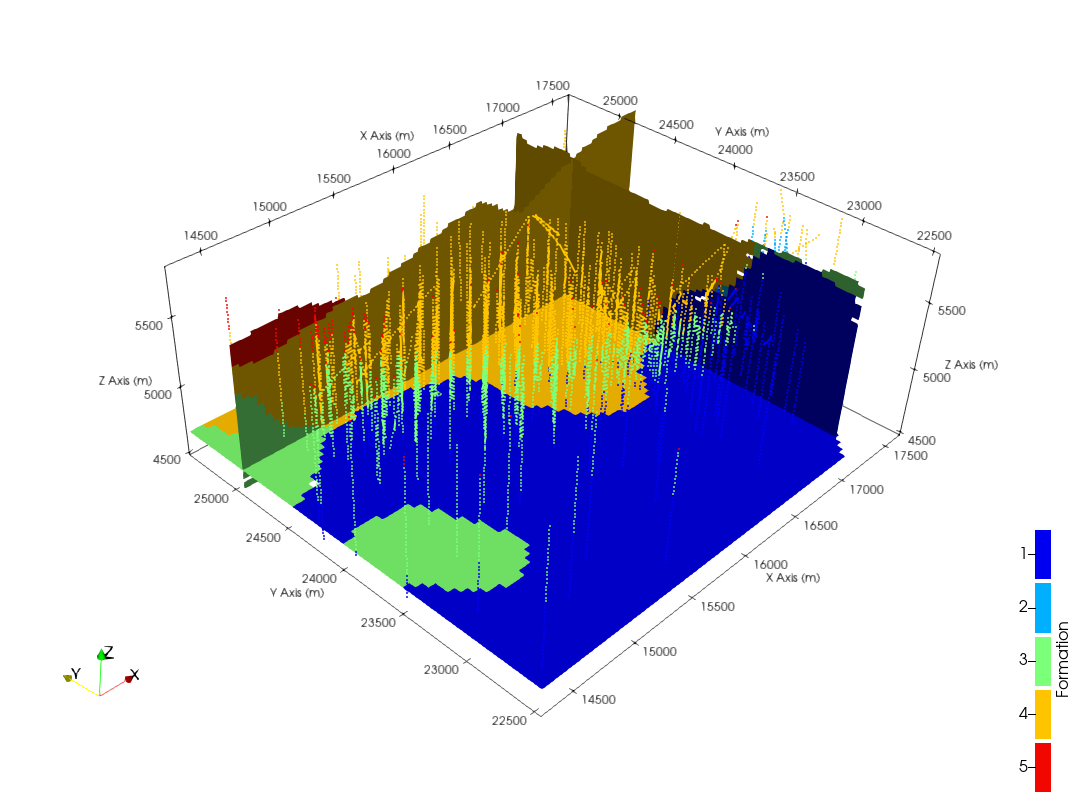
\includegraphics[width=0.45\textwidth]{capitulo_3/imagens/real2.png}\label{fig:g2}}
\end{figure}

\subsection{Discussão}

Uma das técnicas tradicionalmente usadas para modelar geocorpos e avaliar sua incerteza na presença de várias categorias é a simulação sequencial dos indicadores (SISIM). A SISIM foi aplicada ao mesmo banco de dados a fim de comparar os resultados com a metodologia proposta, uma vez que também depende apenas das coordenadas x, y e z dos compósitos e da propriedade categórica. 

A \autoref{sec_comp} mostra um comparativo de seções verticais XZ entre a metodologia proposta (\autoref{fig:explicit}), a SISIM (\autoref{fig:sisim}) utilizando o variograma dos indicadores mostrados na \autoref{ouro_vargs}, e um modelo explícito (\autoref{fig:explicit}) elaborado por um geomodelador experiente. Uma animação mostrando as mesmas seções para todas as dez realizações pode ser vista \href{https://github.com/robertorolo/assessing_geological_model_uncertainty_with_probability_fields/blob/main/ezgif-2-802d466feae1.gif}{aqui}. A SISIM gera realizações com uma textura típica \textit{"salt and pepper"} e padrões ruidosos, o que não é geologicamente realista. Enquanto a metodologia proposta cria limites contínuos que são mais semelhantes à interpretação do geomodelador. A ausência de dados de sondagem é responsável pelas regiões onde a metodologia proposta e o SISIM divergem da interpretação do geomodelador. Como o interpolador é global não há necessidade configurar estratégia de busca na metodologia proposta ao contrário da SISIM, entretanto, é necessário definir um variograma adicional para a simulação não condicional, em relação aos variogramas para interpolar as distâncias assinaladas ou simular os indicadores na SISIM. Ao contrário da SISIM o algoritmo não possui mecanismo para respeitar as proporções e reproduzir a continuidade espacial de cada categoria, embora isso possa ser contornado alterando iterativamente os parâmetros e verificando os resultados.

\begin{figure}[H]
    \caption{Comparativo de seções verticais xz entre a metodologia proposta, a SISIM e um modelo explícito.} \label{sec_comp}
     \centering
     \subfloat[][Modelo explícito.]{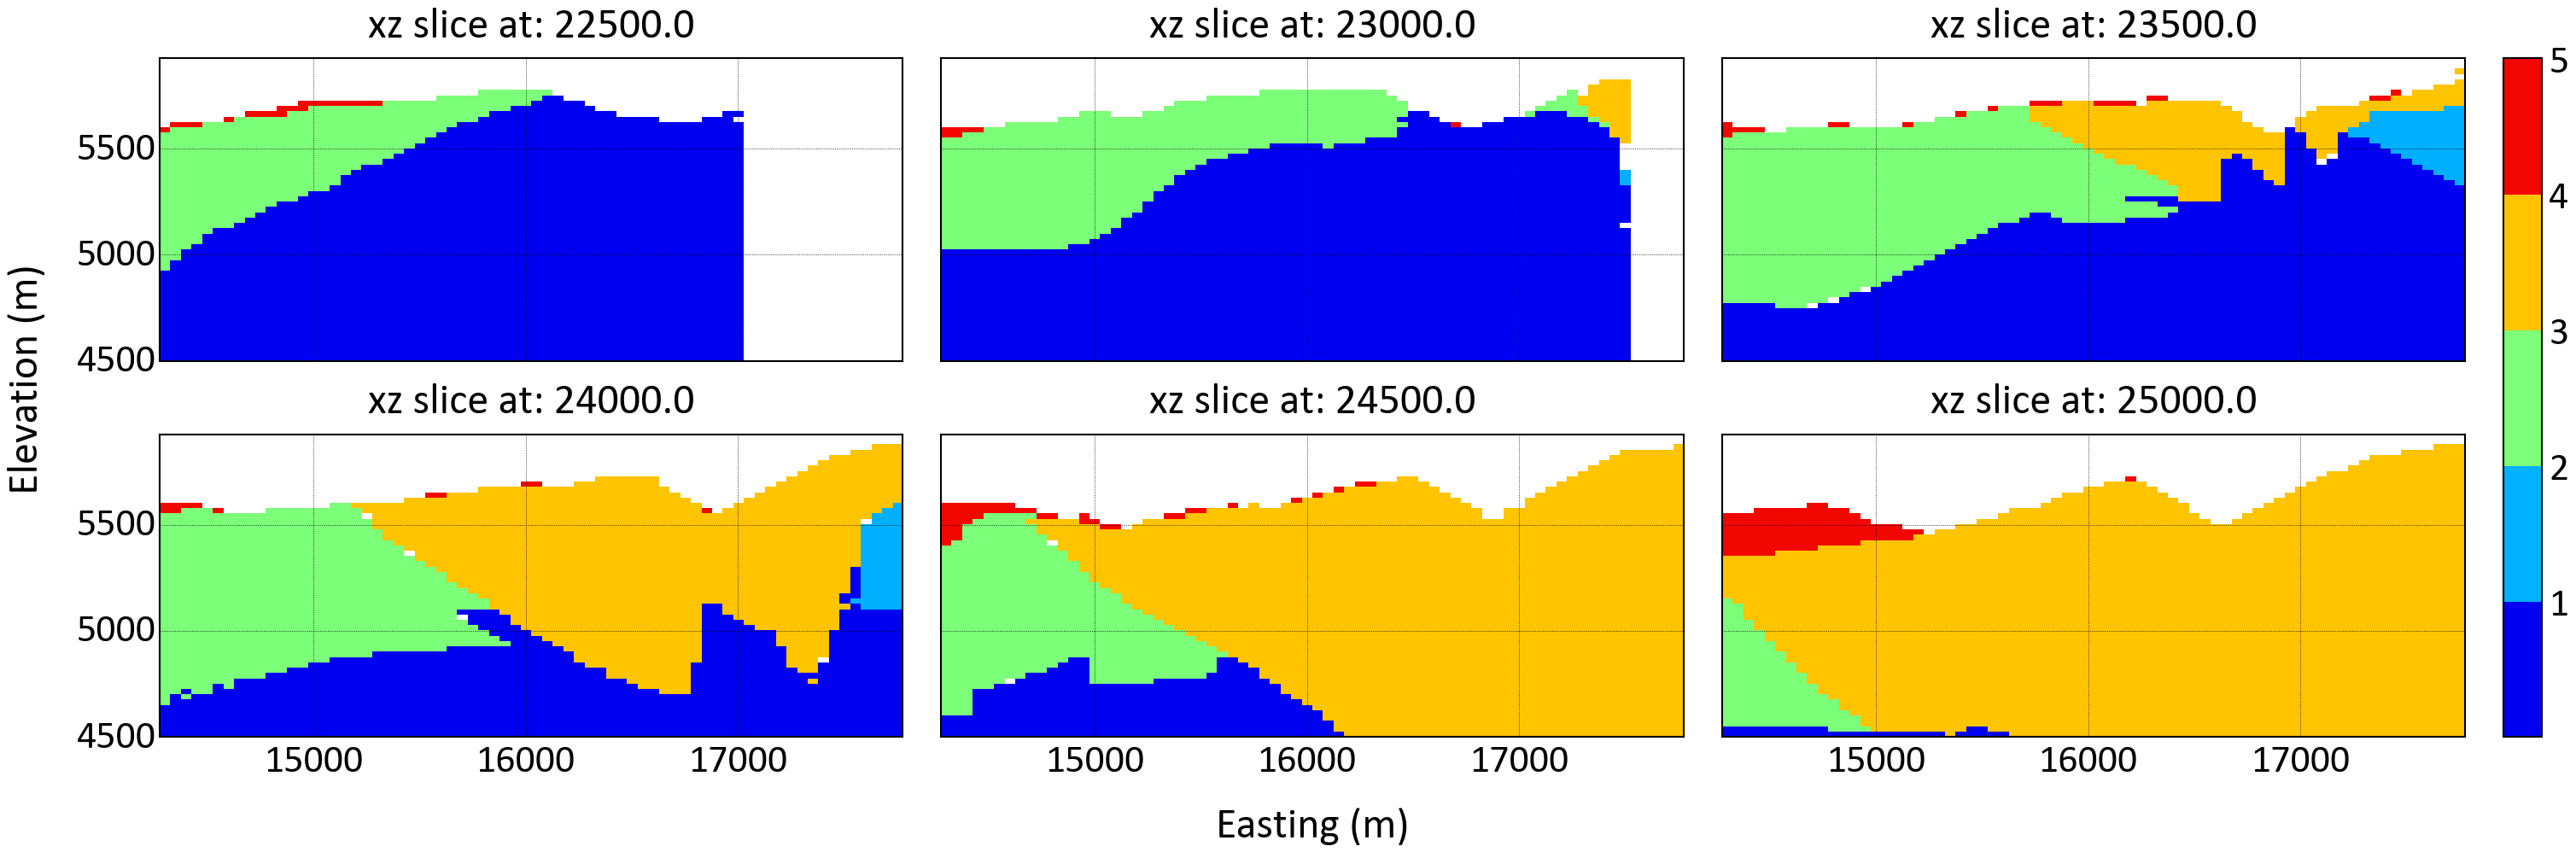
\includegraphics[width=0.8\textwidth]{capitulo_3/imagens/explicit_slicces.png}\label{fig:explicit}}
     \\
     \subfloat[][Metodologia proposta.]{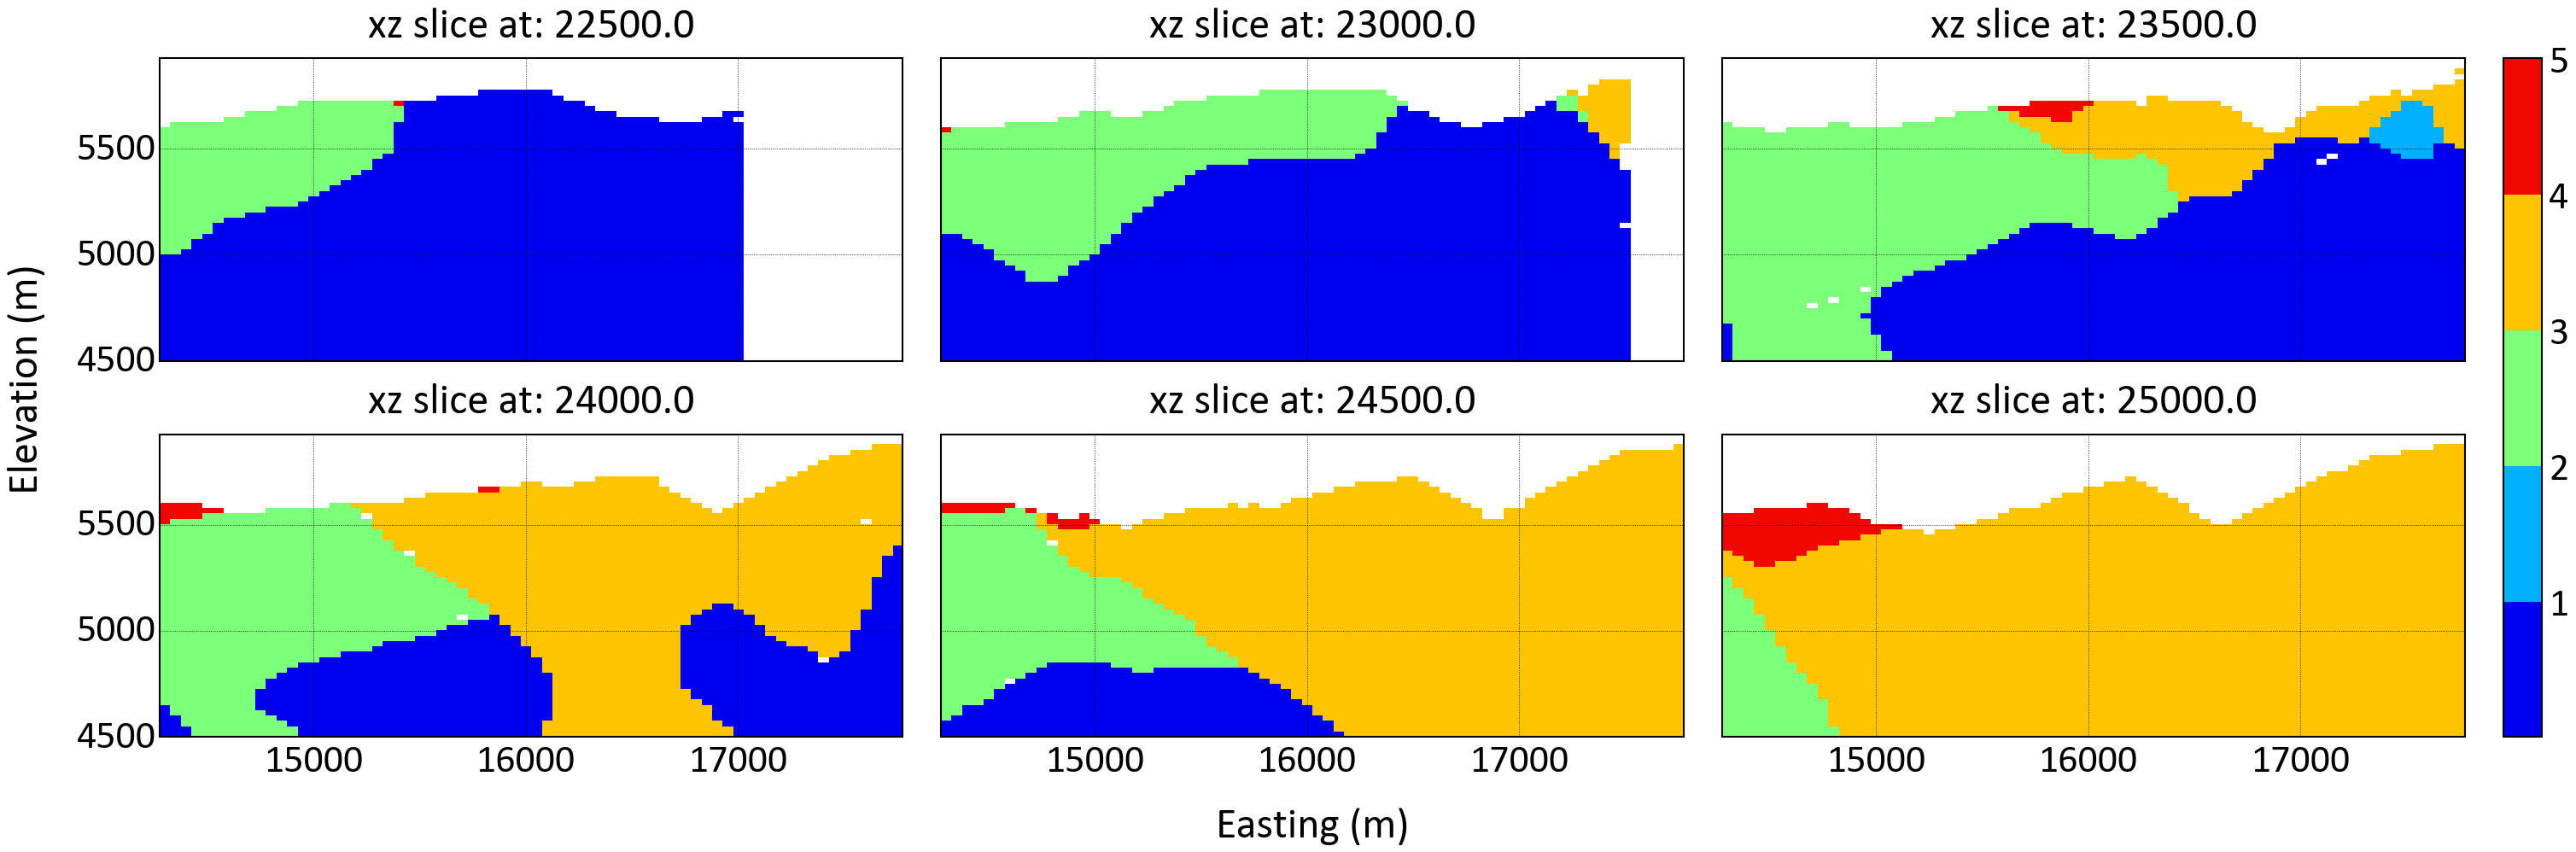
\includegraphics[width=0.8\textwidth]{capitulo_3/imagens/pfields_real_0.png}\label{fig:pfields}}
     \\
     \subfloat[][SISIM.]{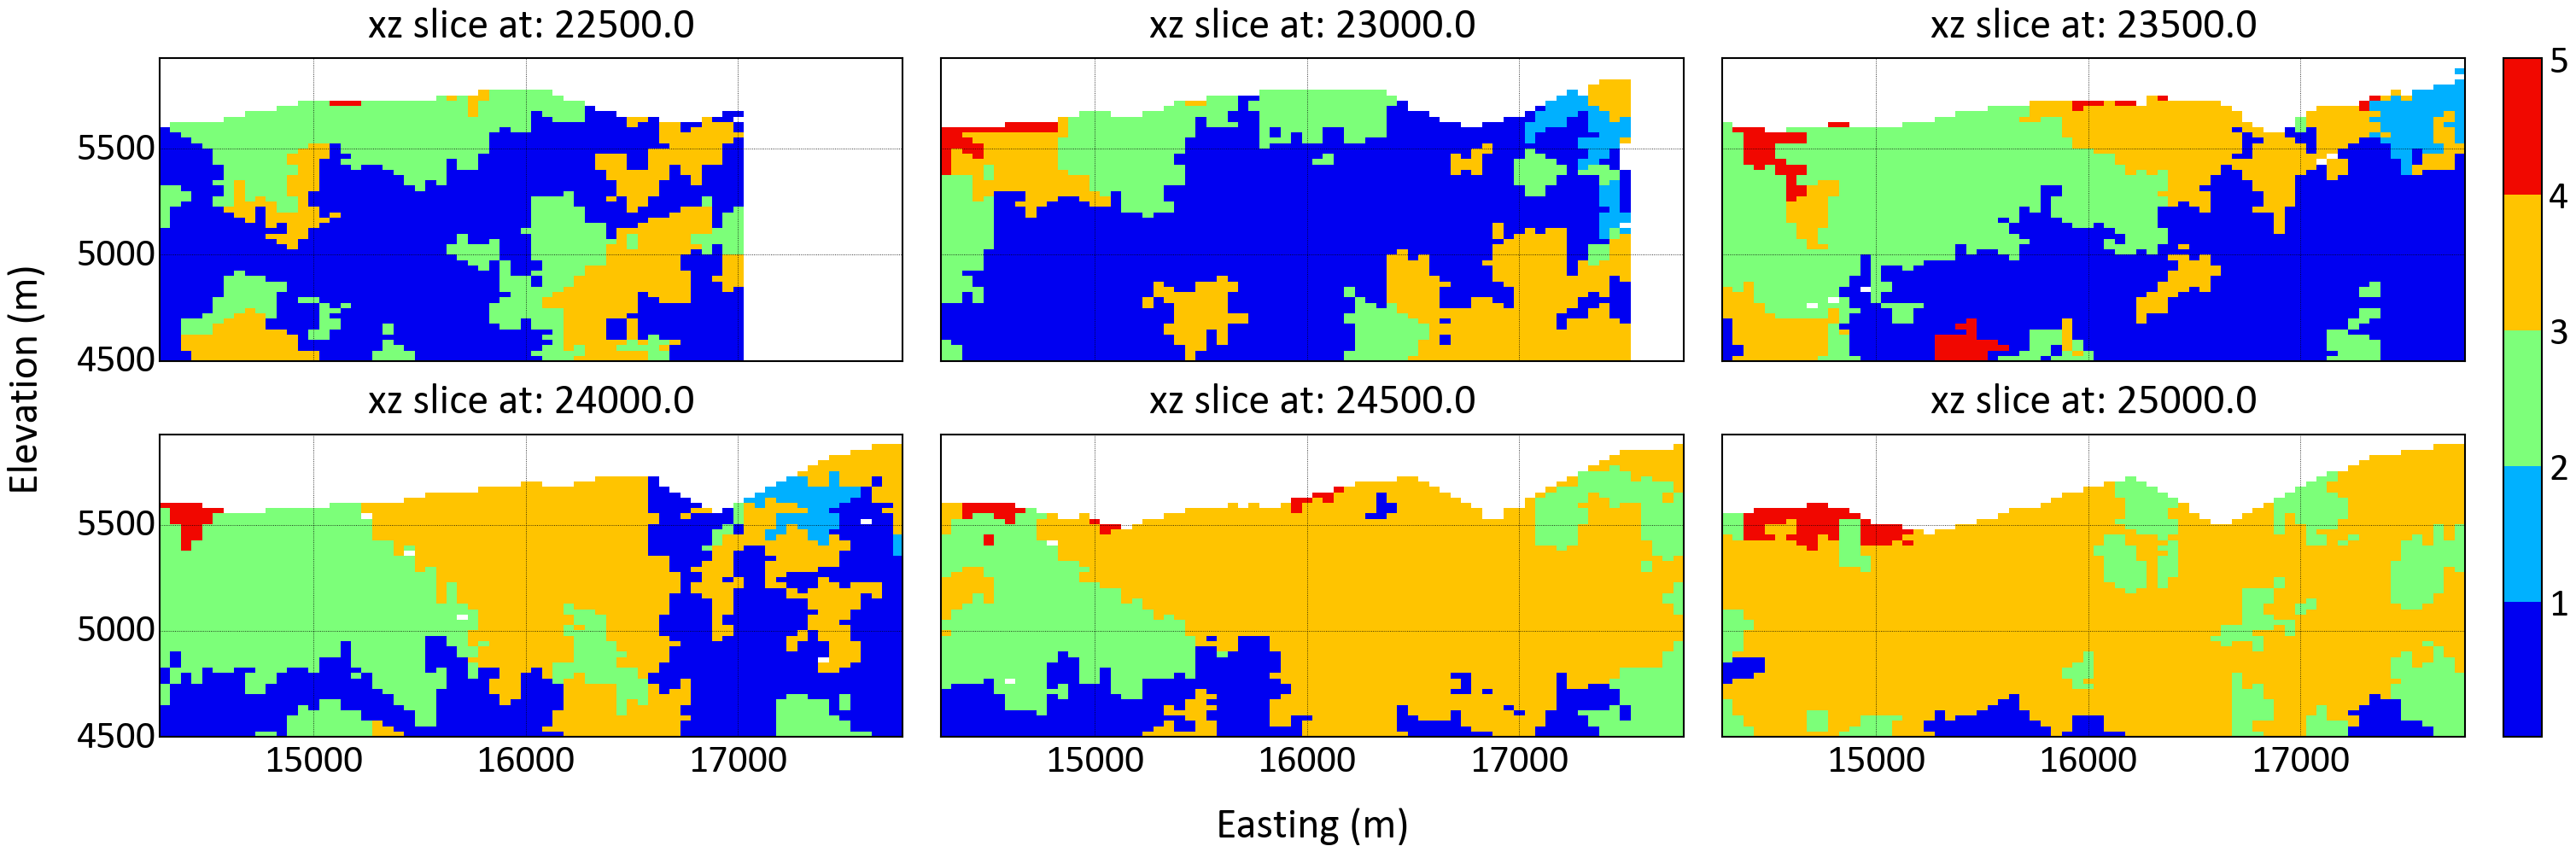
\includegraphics[width=0.8\textwidth]{capitulo_3/imagens/sisim_real_0.png}\label{fig:sisim}}
\end{figure}

O comportamento dos contatos é controlado pelo variograma usado na simulação não condicional; alcances menores e efeitos pepita maiores geram limites irregulares e descontínuos. Por outro lado, longos alcances e pequenos efeitos pepita geram limites suaves e contínuos. A \autoref{sph_jura} mostra uma realização para o \textit{Swiss Jura} criada usando um variograma esférico com um alcance de 50 metros. Os contatos são mais ásperos do que aqueles vistos na \autoref{reals_pfield_jura}, que foram gerados por um variograma Gaussiano.

\begin{figure}[H]
	\caption{\label{sph_jura} Uma realização para o \textit{Swiss Jura} criada usando um variograma esférico para a simulação não condicional.}
	\centering
		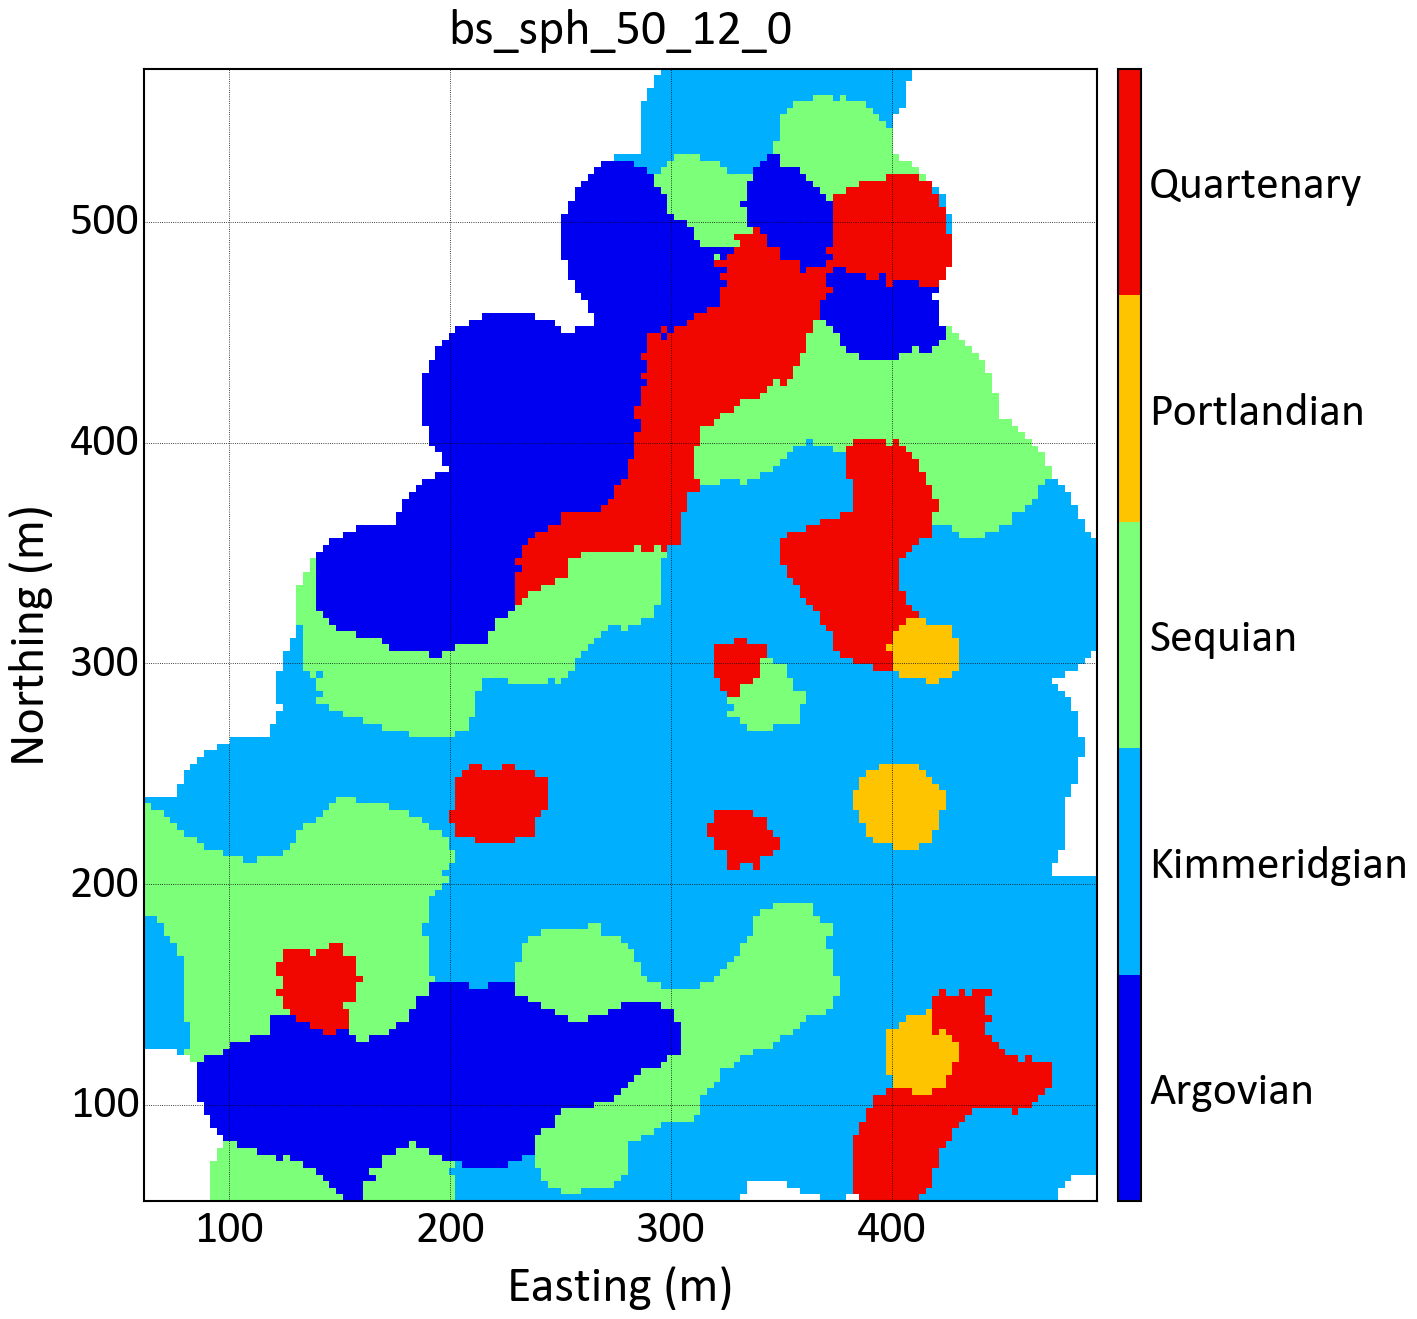
\includegraphics[width=0.6\textwidth]{capitulo_3/imagens/sph_real_0_50_12.png}
\end{figure}

A magnitude da incerteza é controlada tanto pela largura de zona de incerteza quanto pelo parâmetro $\omega$. Um valor para o parâmetro $omega$ pode ser escolhido para todos os blocos ou o maior valor absoluto entre as distâncias assinaladas pode ser utilizado como parâmetro $omega$ bloco a bloco, nesse caso somente a largura da banda vai controlar a magnitude da incerteza. Uma animação mostrando 10 realizações feitas para o \textit{Swiss Jura} com o mesmo variograma Gaussiano do exemplo anterior, entretanto, para uma largura da zona de incerteza de 20 metros pode ser vista \href{https://github.com/robertorolo/assessing_geological_model_uncertainty_with_probability_fields/blob/main/ezgif-2-721b458d5c70.gif}{aqui}. Como há mais área para os contatos mudarem de posição, a variação de área é maior do que a observada para a largura de banda de 12 metros. 

O mesmo comportamento é evidenciado pelos mapa de entropia calculados a partir da \autoref{shannon_entr} (e estandardizadas para que os valores estejam entre 0 e 1) para as bandas de incerteza de 12 e 20 metros. Blocos onde a entropia tem um valor alto variam mais entre diferentes categorias nas diferentes realizações. 

\begin{figure}[H] 
    \centering
    \caption{Entropia calculada a partir das dez realizações no \textit{Swiss Jura}.} \label{jura_entropy}
     \subfloat[][Zona de incerteza de 12 metros.]{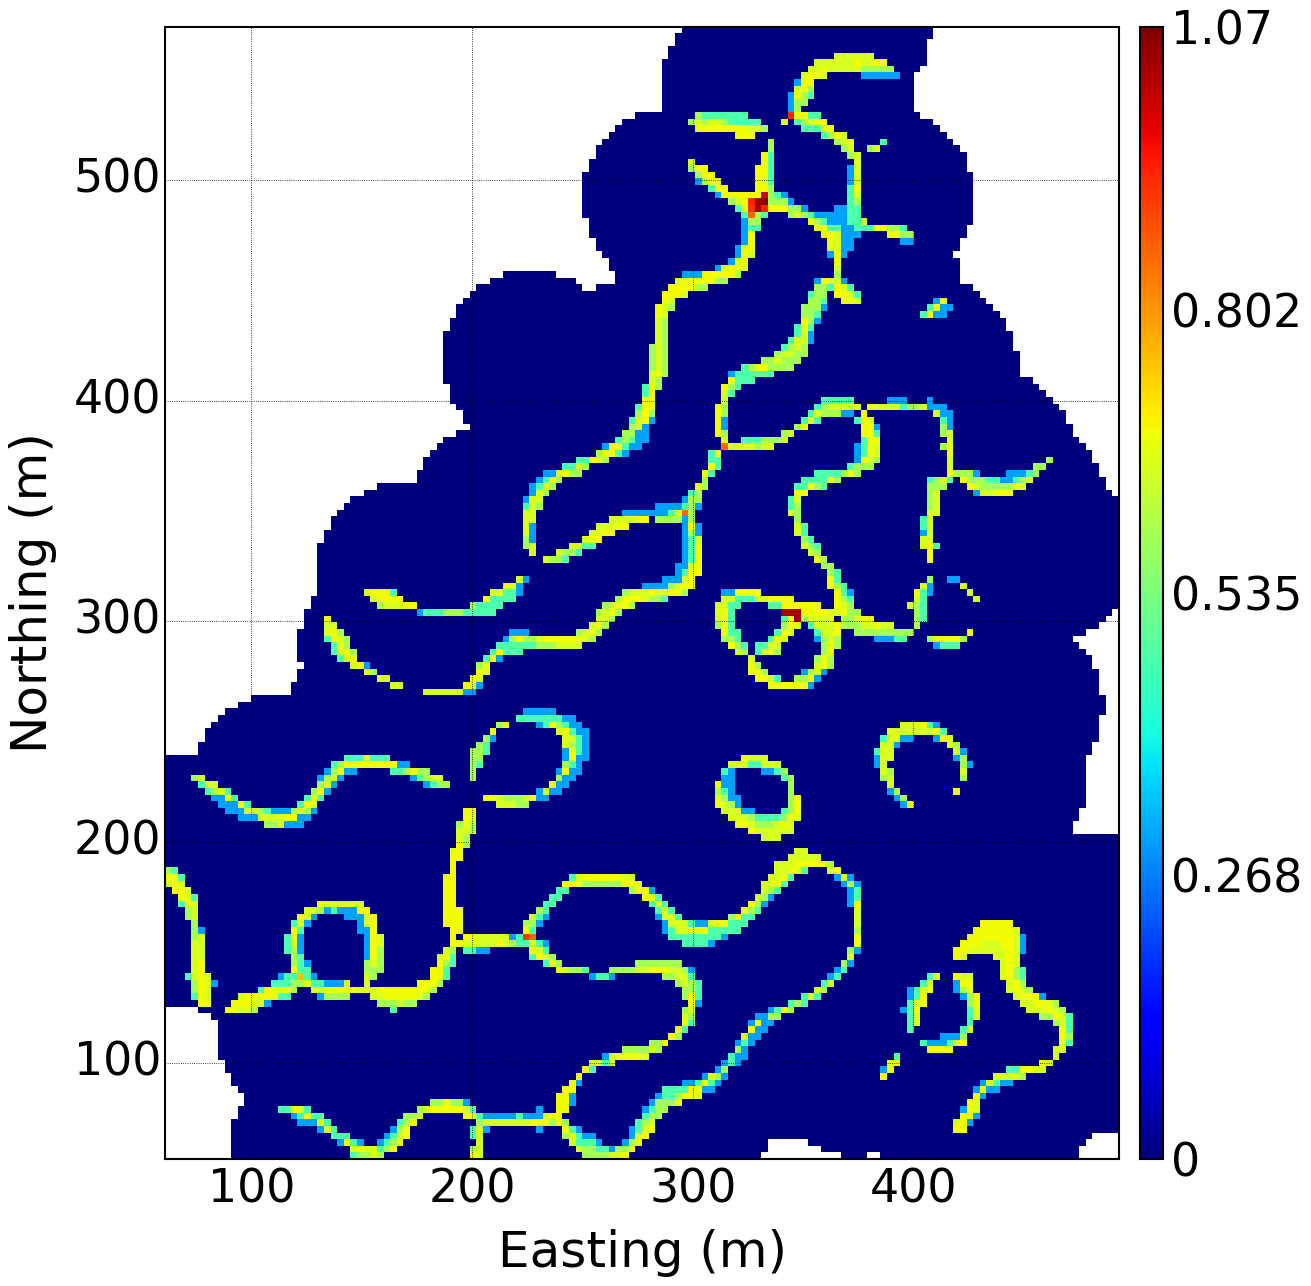
\includegraphics[width=.45\textwidth]{capitulo_3/imagens/jura_entropy_12.png}\label{<figure1>}}
     \hspace{1em}
     \subfloat[][Zona de incerteza de 20 metros.]{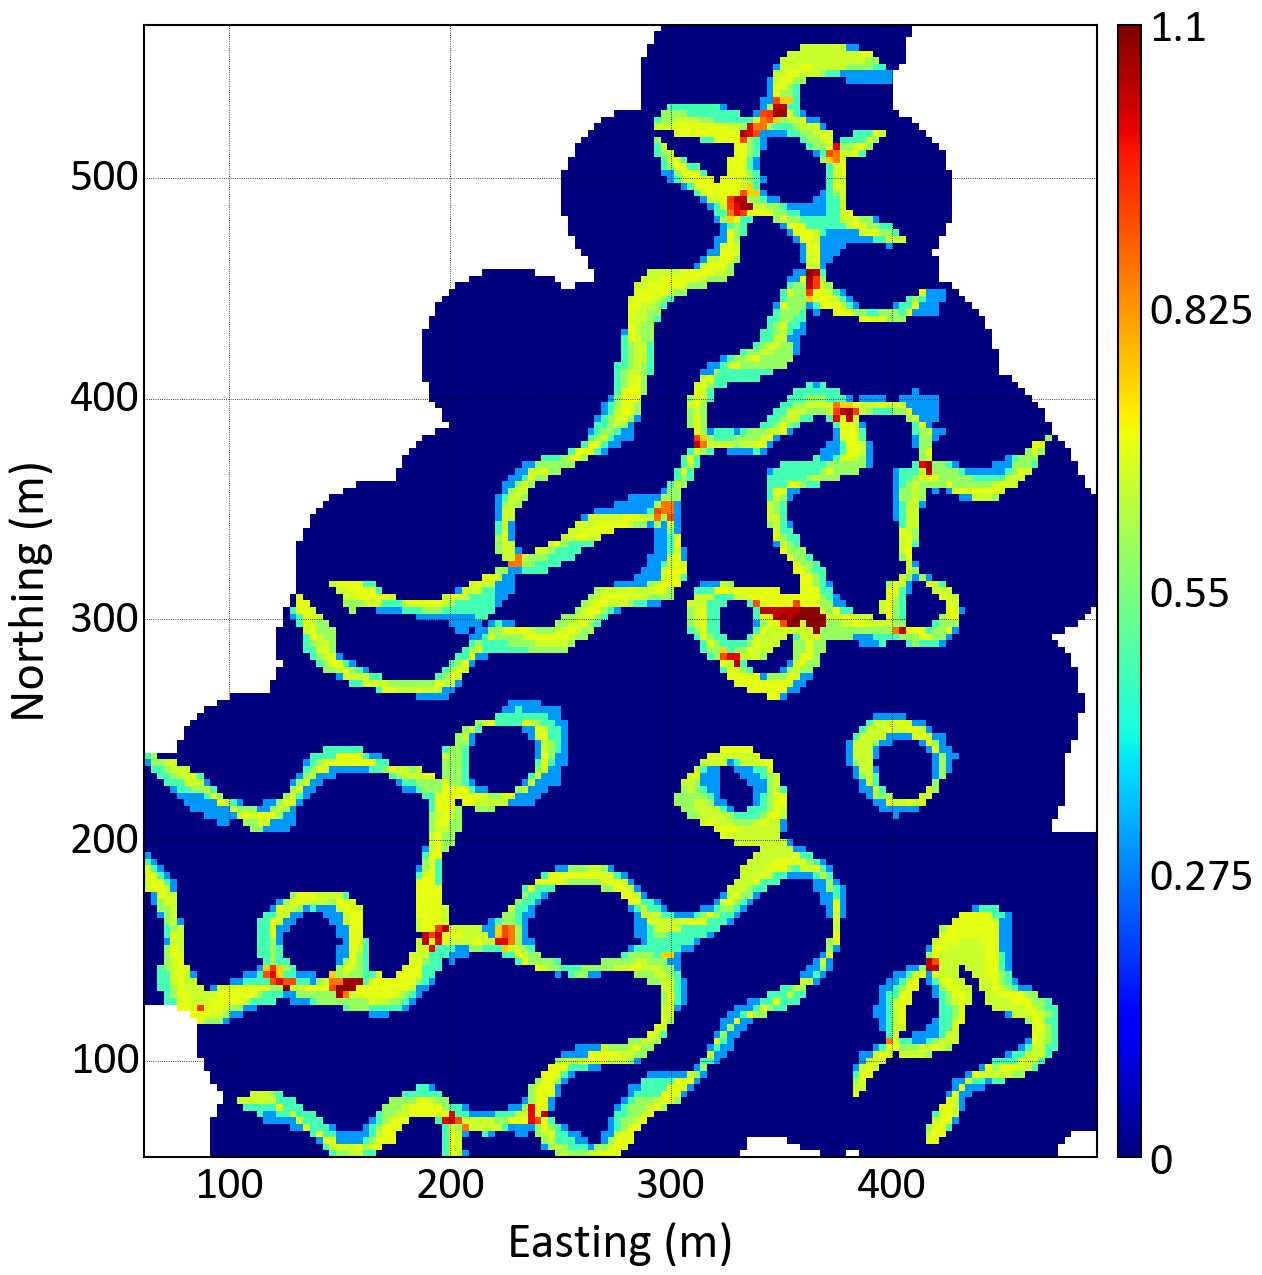
\includegraphics[width=.45\textwidth]{capitulo_3/imagens/jura_entropy_20.png}\label{<figure2>}}
\end{figure}

A \autoref{areas_jura} mostra a área para as categorias Swiss Jura para 10 realizações com larguras de banda de 12 e 20 metros. Os desvios padrão das áreas também são mostrados. O gráfico mostra que as áreas têm maior variação para todas as categorias quando a largura de banda da incerteza é de 20 metros.

\begin{figure}[H]
	\caption{\label{areas_jura} Variação de volume para todas as categorias do \textit{Swiss Jura} para 10 realizações com larguras de banda de 12 e 20 metros.}
	\centering
		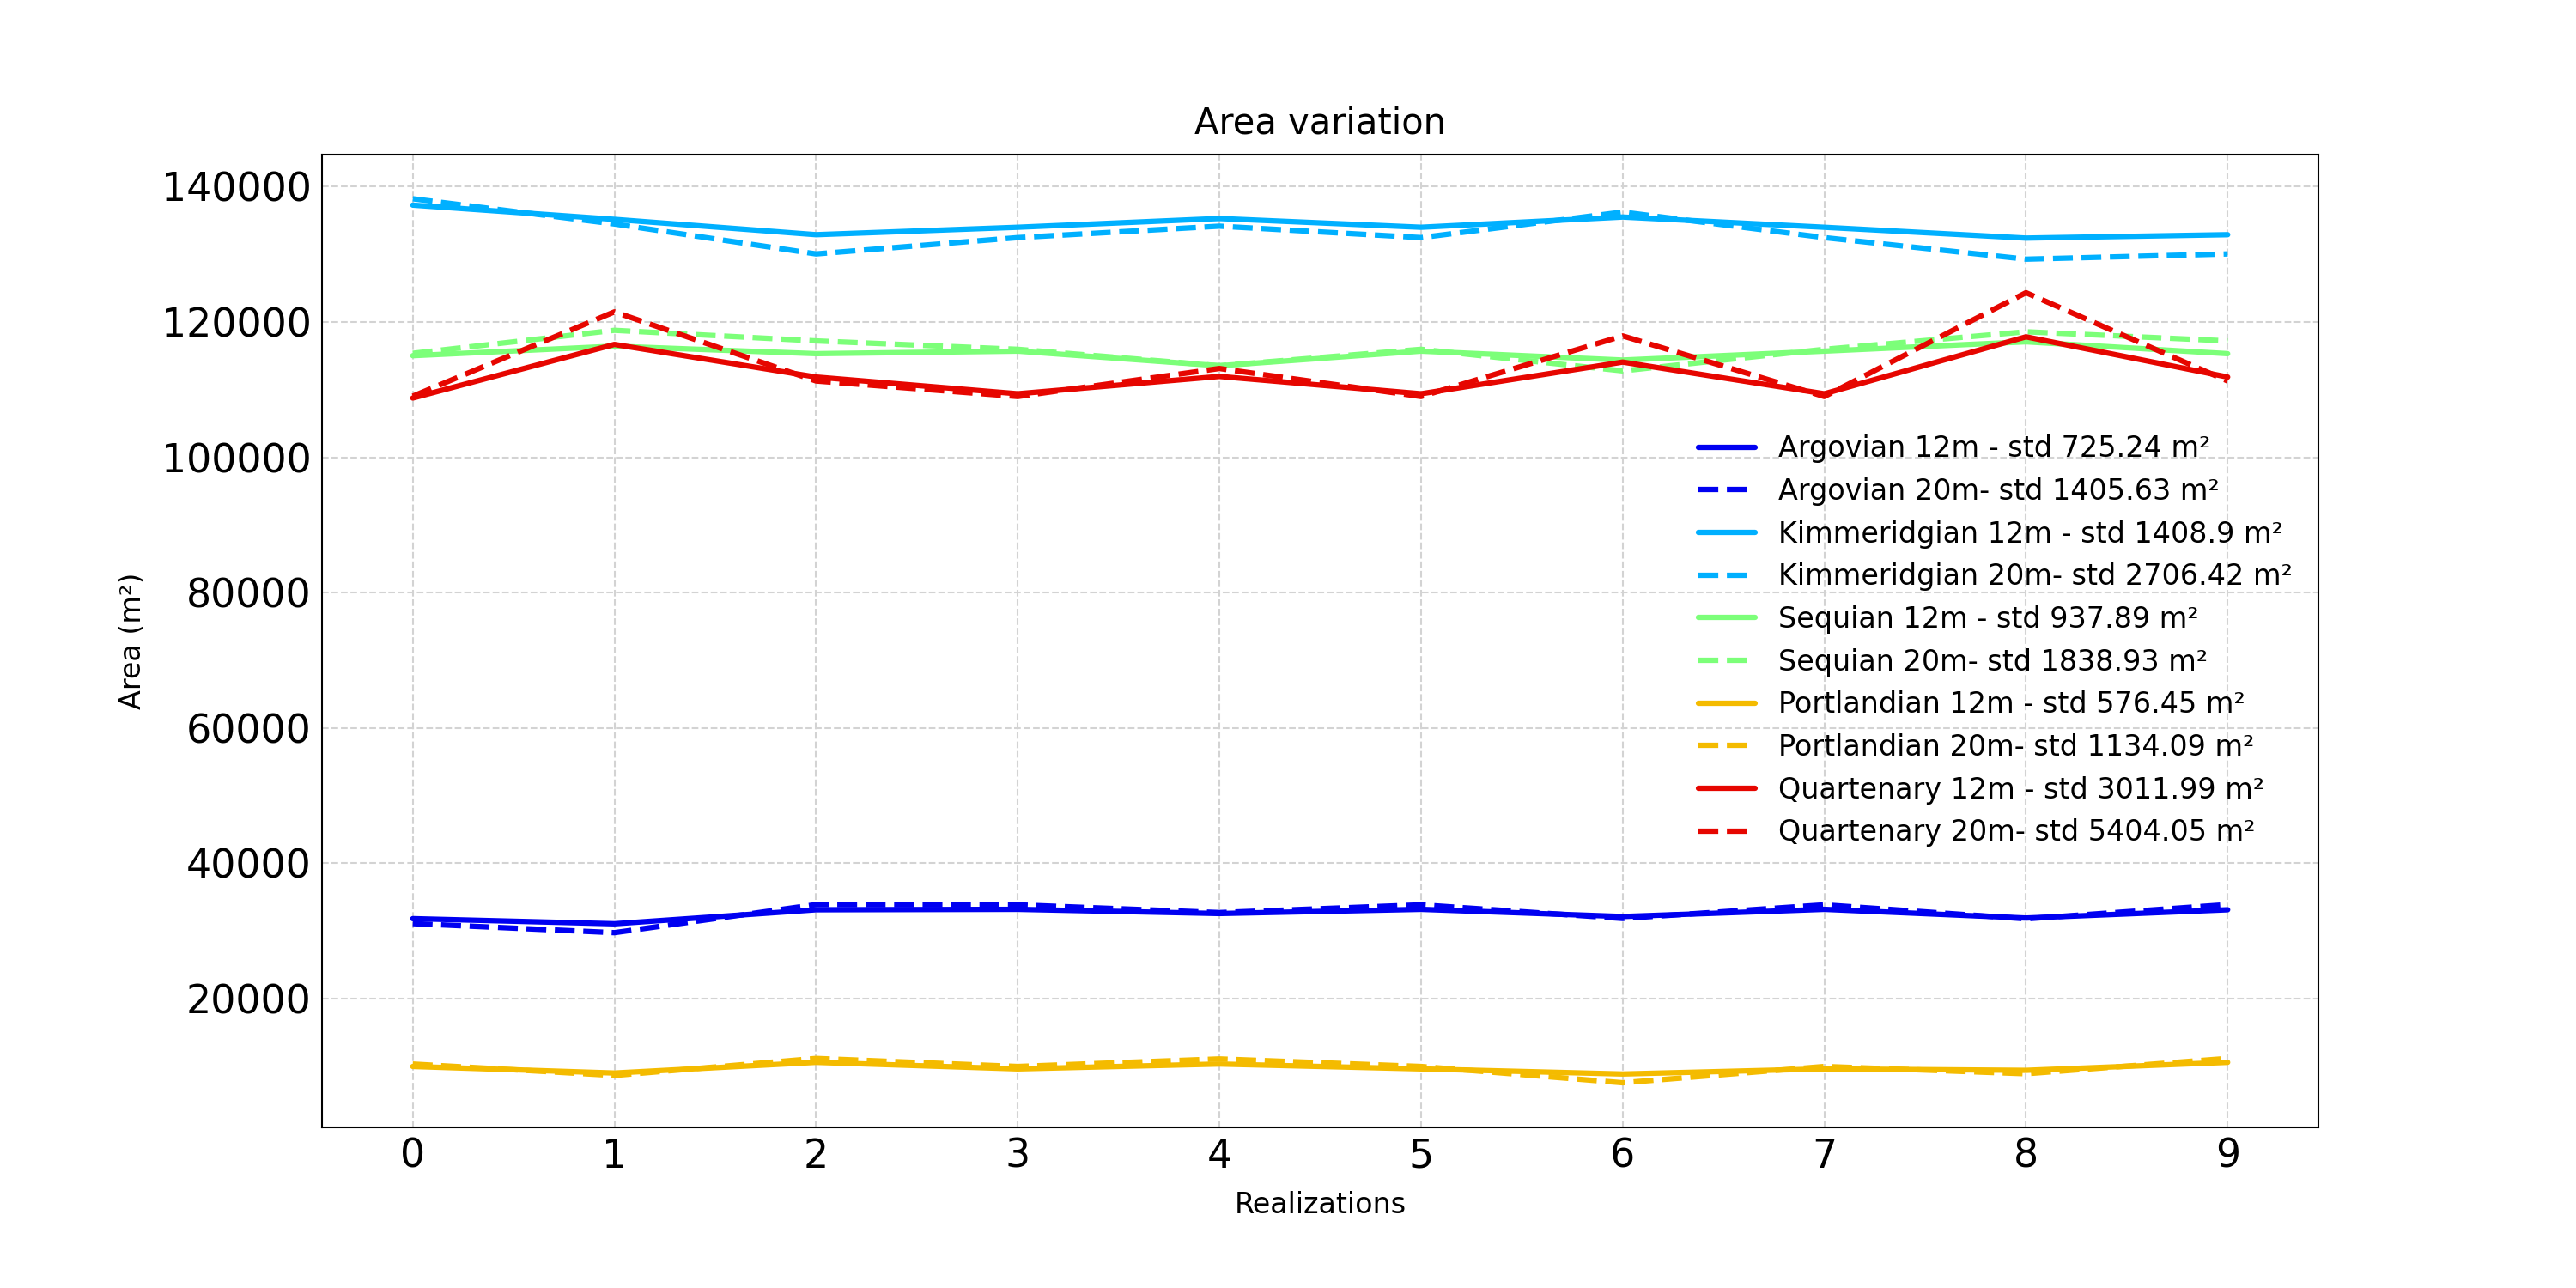
\includegraphics[width=\textwidth]{capitulo_3/imagens/areasjura.png}
\end{figure}

A \autoref{conf_mat_pfields} mostra uma matriz de confusão representando a média da proporção de blocos que reproduzem as amostras mais próximas entre todas as realizações, para todas as categorias no banco de dados. A reprodução é alta para categorias de alto volume com abundância de amostras. As categorias 2 e 5 têm menos volume e menos amostras em comparação com as categorias 1, 3 e 4, o que explica a menor reprodução. Para a categoria 5, o problema é acentuado, uma vez que existem apenas algumas amostras esparsas na superfície do depósito. A distância estimada das categorias de volume maior sempre será mais negativa nessas áreas para casos como esse. Uma maneira de contornar esse problema é pré-processar os modelos atribuindo as categorias das amostra mais próximas aos blocos correspondentes. Esta solução congelaria alguns blocos com base no valor da amostra mais próxima, minimizando o desvanecimento dessas categorias em relação à se fossem interpoladas/simuladas com dados circundantes.

\begin{figure}[H]
	\caption{\label{conf_mat_pfields} Matriz de confusão mostrando a média da proporção de blocos que reproduzem as amostras mais próximas entre todas as realizações para todas as categorias do banco de dados.}
	\centering
		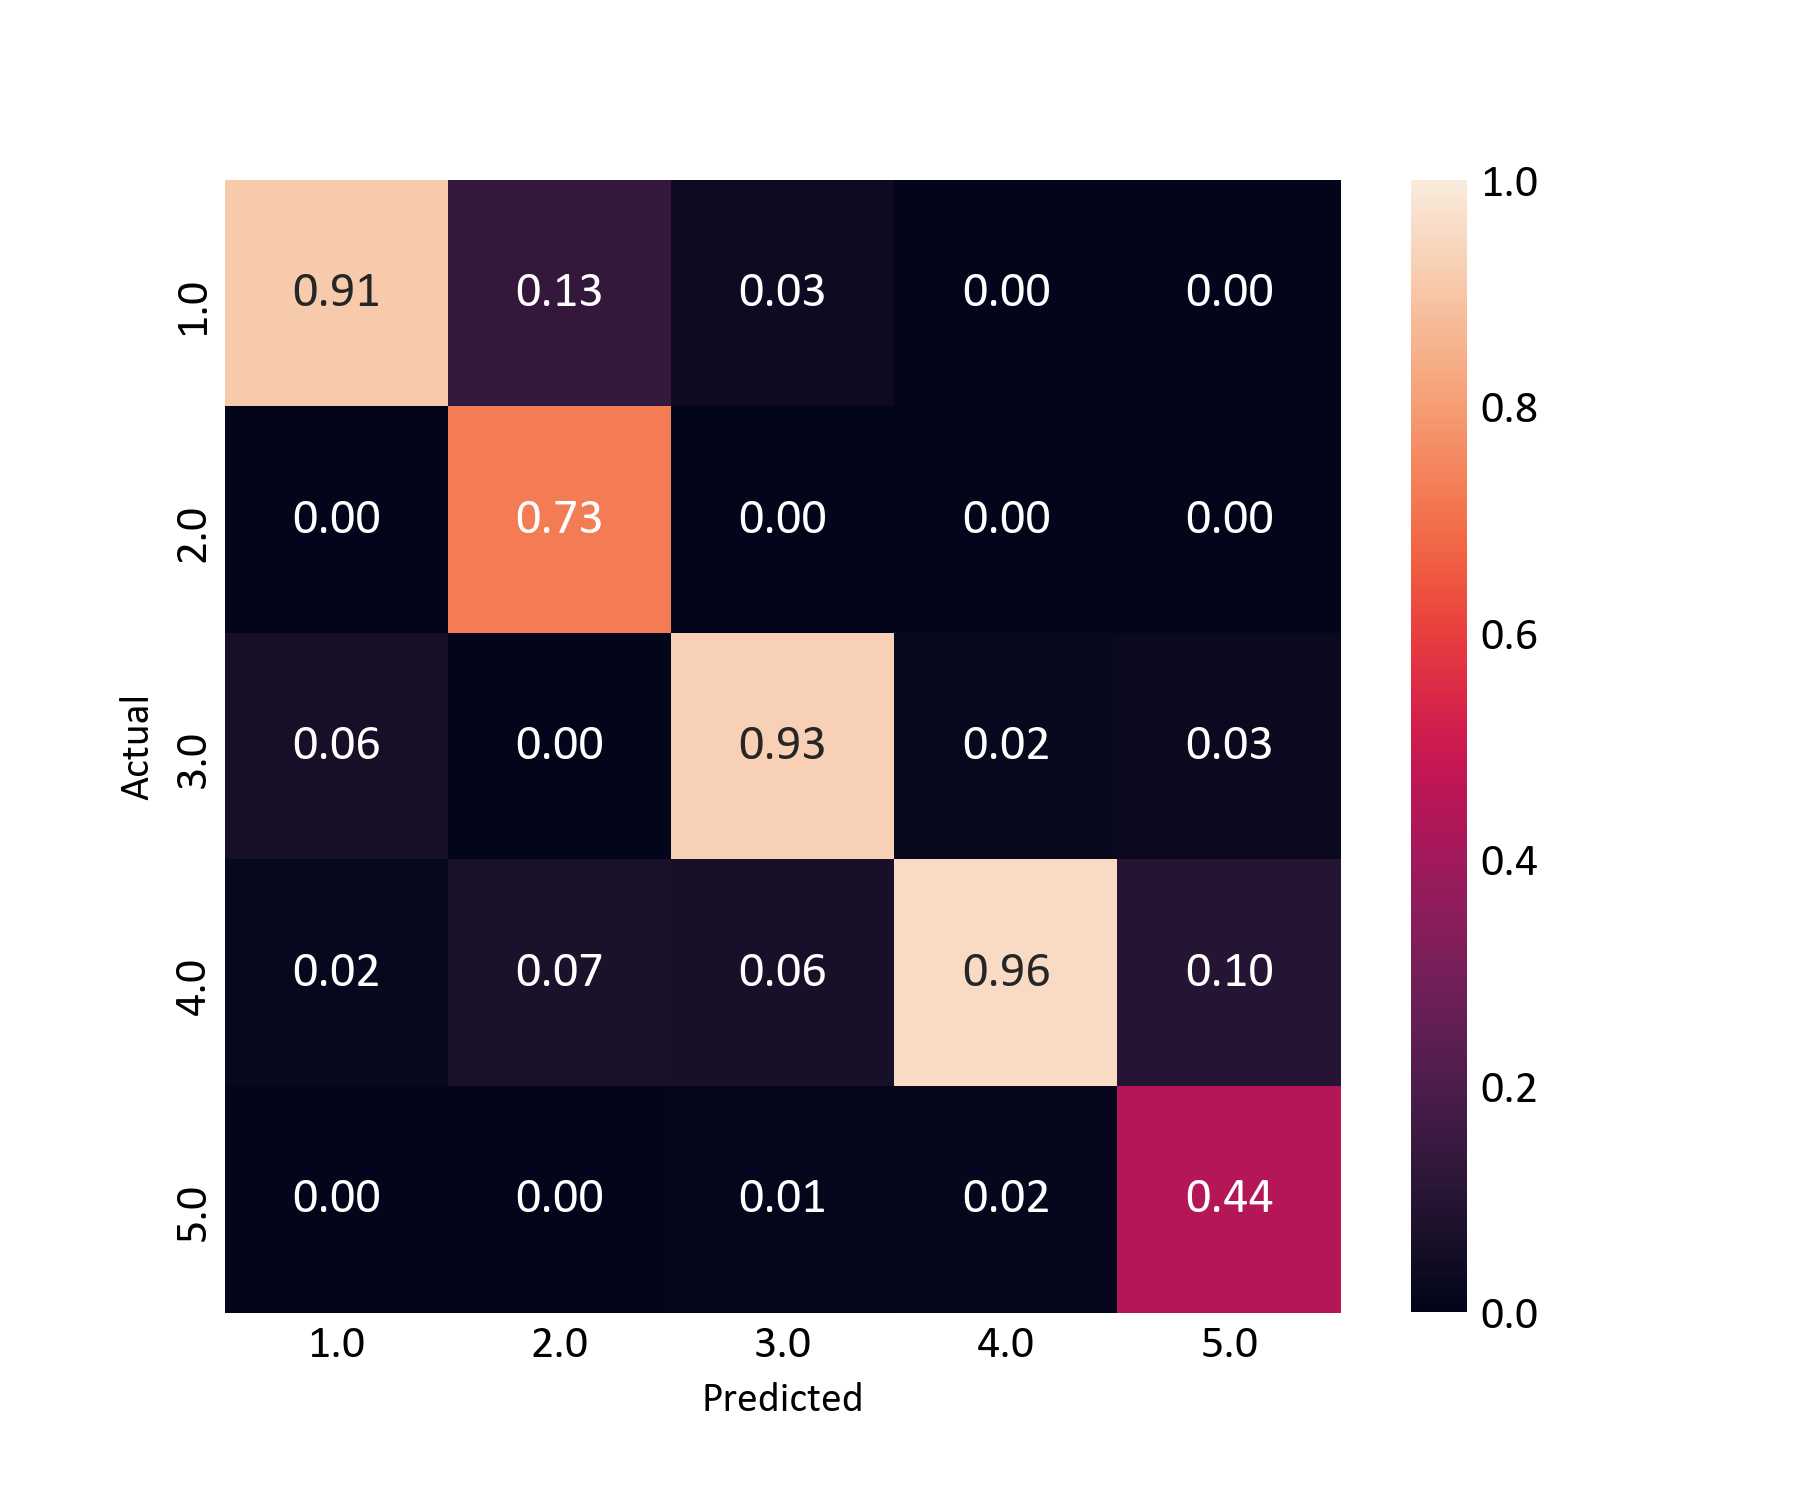
\includegraphics[width=0.6\textwidth]{capitulo_3/imagens/backflag.png}
\end{figure}

O método é bastante simples e conveniente já que dissocia a simulação dos contatos da obtenção de probabilidades locais. Geralmente, as probabilidades foram calculadas previamente para a construção de um modelo geológico determinístico. Assim, para avaliação da incerteza é necessário apenas realizações de uma simulação não condicional. Entretanto, não há uma forma objetiva para definição do variograma das simulações. Além disso, uma mesma simulação com o mesmo variograma, para representar o contato entre todas as diferentes categorias do depósito mineral pode ser restritivo. O contato entre horizontes sulfetados e oxidados podem apresentar um contato suave, enquanto o contato entre rochas intrusivas podem ser mais ásperos em depósitos de cobre pórfiro por exemplo.

A zona de incerteza simétrica ao redor dos contatos também pode ser um fator de restrição de aplicabilidade do método. Considerar uma zona simétrica, embora simplifique o método, não leva em consideração a possibilidade de que amostras podem estar no interior da zona de incerteza. Além disso, pode haver uma maior incerteza em relação a alguns contatos em relação aos demais, nesse sentido, existe a necessidade de zonas de incerteza com espessuras diferentes para diferentes contatos.

\section{Simulação hierárquica dos contatos}\label{hier_bound_sim}

A proposta dessa metodologia é avaliar a incerteza do modelo geológico multi-categórico simulando os contatos entre os diferentes domínios com base no método proposto por \citeonline{wilde2012kriging}. Os resultados são obtidos a partir dos furos de sondagem compositados, apresentando coordenadas X, Y e Z e propriedade categórica que representa as diferentes litologias do depósito. O método de \citeonline{wilde2012kriging} pode ser aplicado apenas a casos binários e fazer sua aplicação ingenuamente em casos de múltiplos domínios é demorado, subjetivo e pode causar sobreposição de blocos atribuídos à diferentes categorias em diferentes realizações ou produzir blocos não atribuídos à nenhuma categoria em algumas das realizações. Por esse motivo essa tese propõe um algoritmo para agrupar automaticamente as diferentes litologias e um fluxo de trabalho para simular cada grupo individualmente e, em seguida, reconstruir o modelo geológico multi-categórico, a partir do agrupamento, de forma hierárquica. 

A metodologia foi inicialmente proposta por \citeonline{amarante_incerteza_associada} e foi posteriormente aprimorada tendo sua subjetividade reduzida e automatização aumentada \cite{amarante2021boundary}. Um outro estudo de caso foi conduzido em um banco de dados de ferro por \citeonline{amarante2019assessing} e o método se mostrou competente, apresentando resultados melhores em relação a outros métodos concorrentes.

A primeira etapa do fluxo de trabalho é definir grupos de amostras que representam os contatos entre as diferentes litologias do depósito mineral. O agrupamento pode ser definido explicitamente por um geomodelador ou pode ser feito automaticamente pelo algoritmo proposto.

O algoritmo de cubos marchantes, apresentado na \autoref{bound_ref}, é aplicado a um proto-modelo geológico para identificar e contar os contatos entre as diferentes litologias. O proto-modelo pode ser criado pelo vizinho mais próximo, máquina de vetores de suporte, krigagem dos indicadores ou usando funções distâncias assinaladas em um \textit{grid} mais grosseiro do que o \textit{grid} de simulação final para acelerar o processo.

A \autoref{fig:jura_proto} mostra um proto-modelo geológico criado a partir do banco de dados \textit{Swiss Jura} usando distâncias assinaladas em um \textit{grid} de 10x10 metros. A resolução do \textit{grid} pode alterar o agrupamento final.

\begin{figure}[H]
    \caption{Proto-modelo e blocos sinalizados como contatos pelo algoritmo cubos marchantes para o \textit{Swiss Jura}.} \label{fig:jura_proto}
     \centering
     \subfloat[][Proto-modelo geológico]{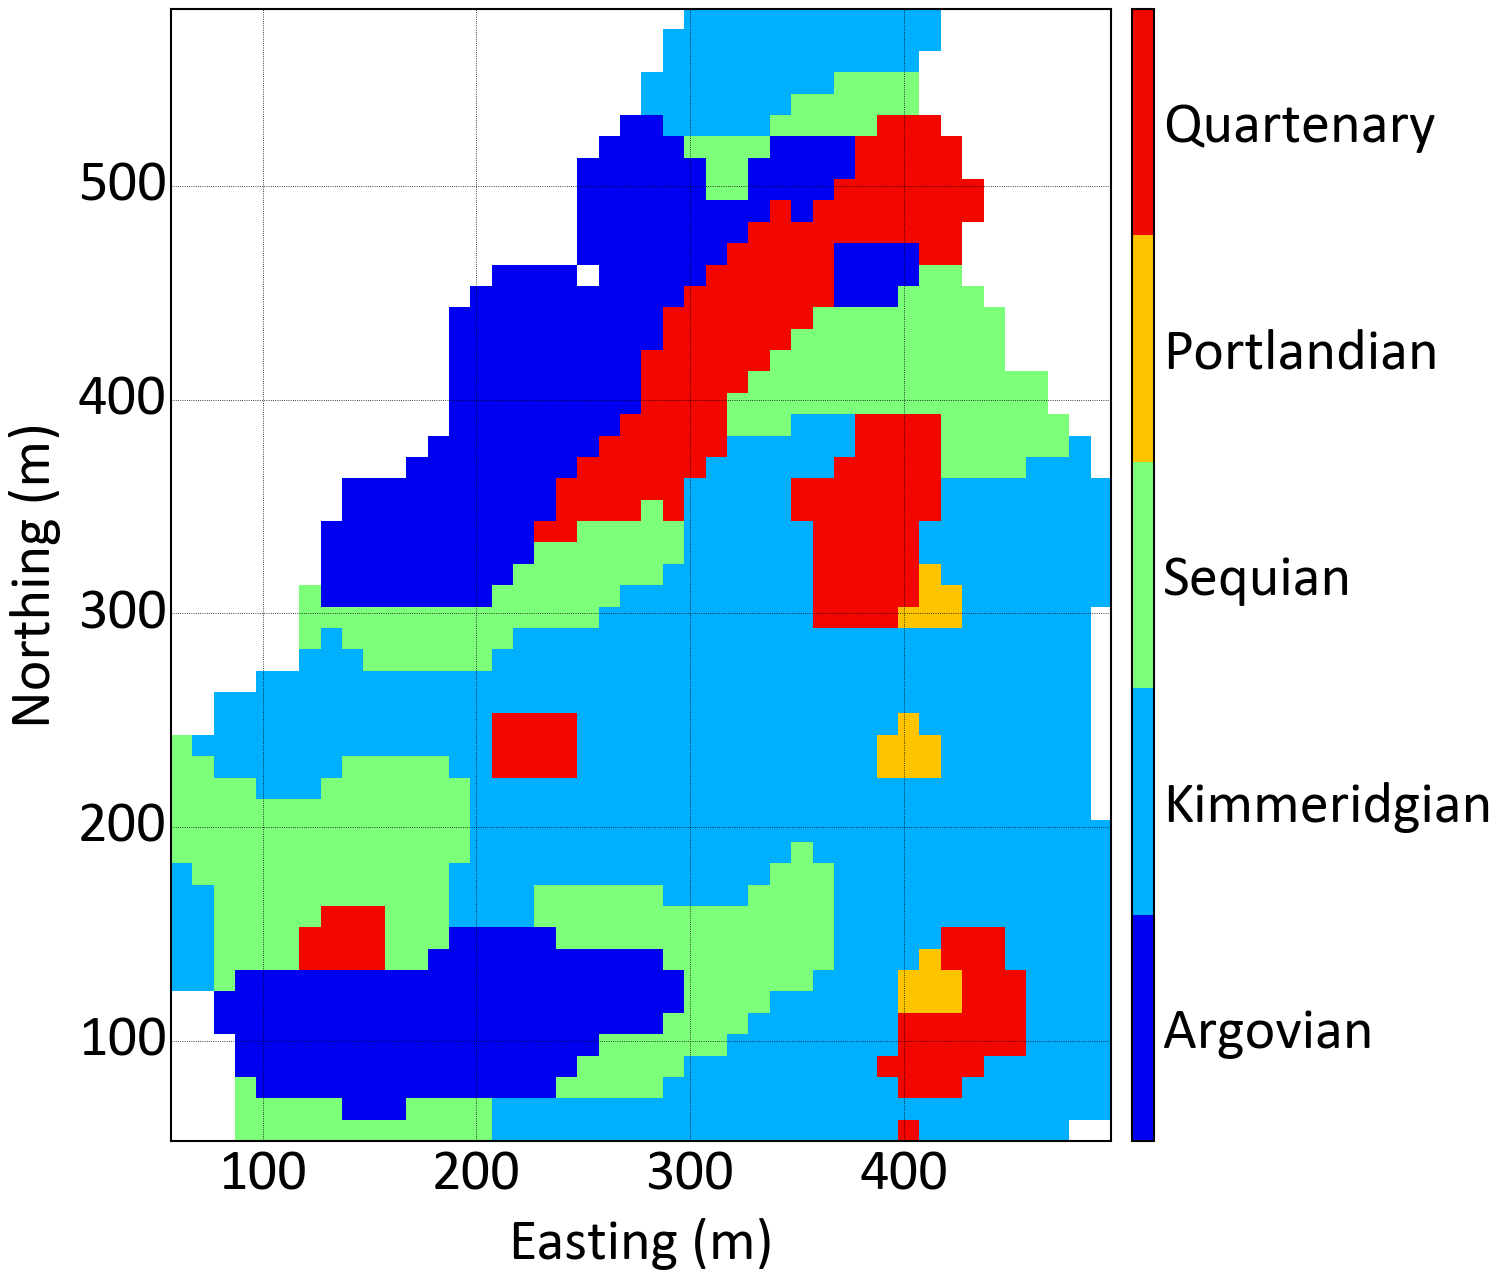
\includegraphics[height=170pt]{capitulo_3/imagens/geomodel.png}\label{fig:proto}}
     \hspace{1em}
     \subfloat[][Blocos sinalizados como contatos. As cores indicam quantas categorias fazem parte desse contato.]{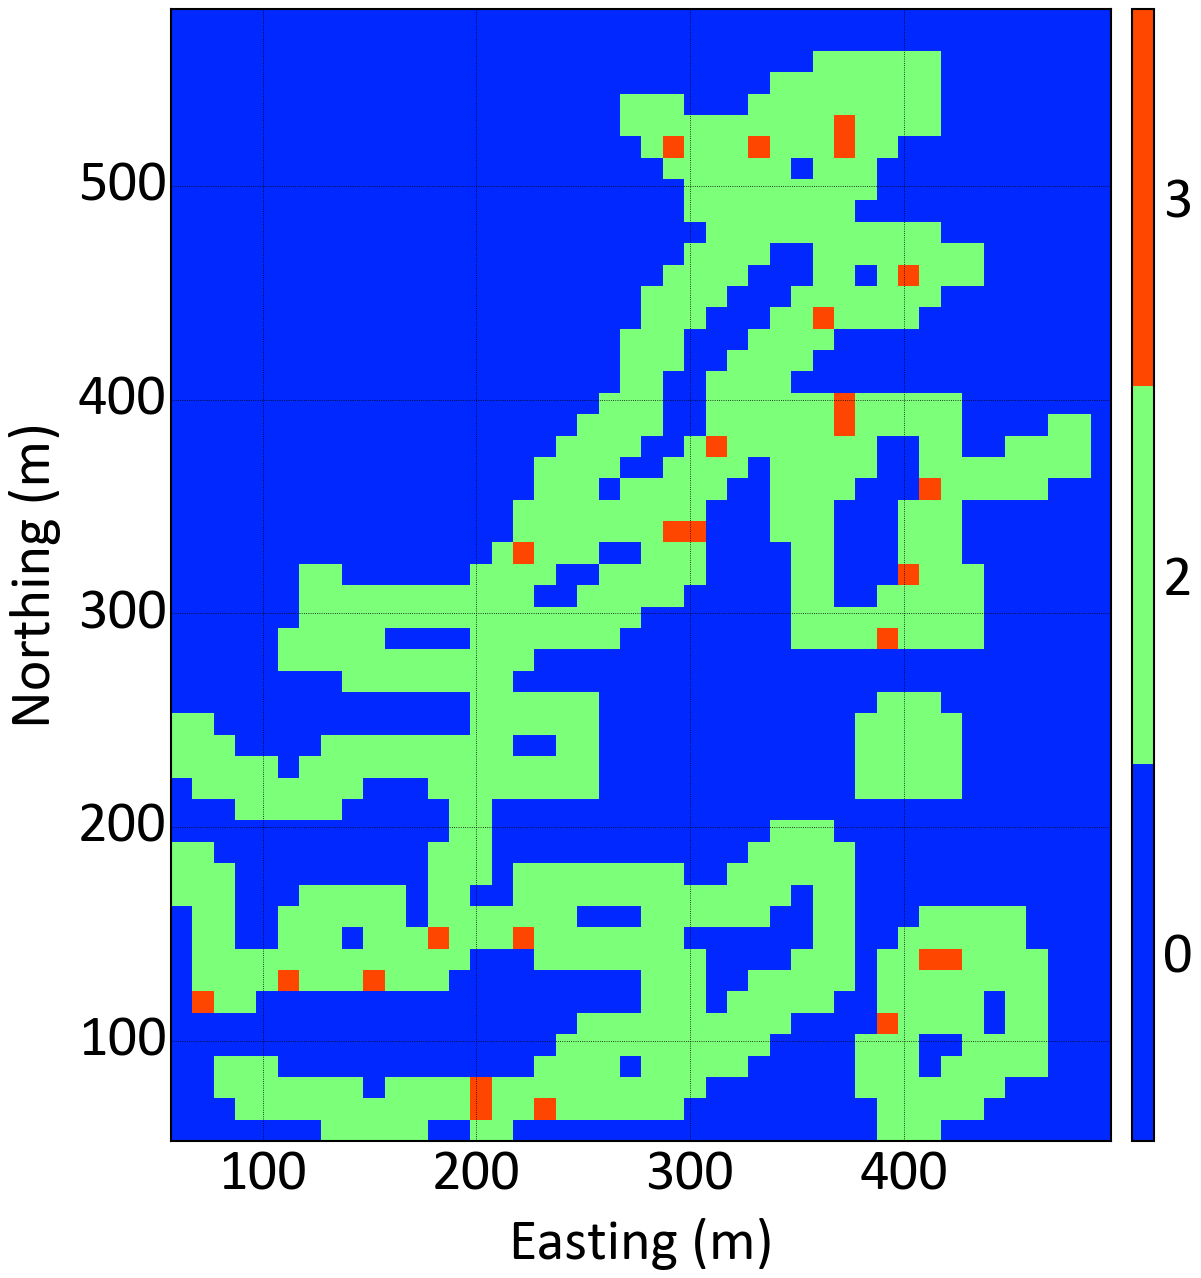
\includegraphics[height=170pt]{capitulo_3/imagens/cdelim.png}\label{fig:contacts}}
\end{figure}

O algoritmo dos cubos marchantes, ao identificar um contato, faz sua contagem e o registra. O número de contatos entre as diferentes litologias, contados pelo algoritmo dos cubos marchantes no proto-modelo da Figura \autoref{fig:proto}, é mostrado na \autoref{table:contact_count}.

\begin{table}[H]
\caption{Contagem de contatos pelo algoritmo dos cubos marchantes.} \label{table:contact_count}
\centering
\begin{tabular}{|l|l|}
\hline
Kimmeridgian; Sequian                 & 134 \\ \hline
Argovian; Sequian                     & 74  \\ \hline
Kimmeridgian; Quartenary              & 66  \\ \hline
Argovian; Quartenary                  & 45  \\ \hline
Sequian; Quartenary                   & 40  \\ \hline
Kimmeridgian; Portlandian             & 23  \\ \hline
Portlandian; Quartenary               & 9   \\ \hline
Argovian; Kimmeridgian                & 8   \\ \hline
Argovian; Kimmeridgian; Sequian       & 7   \\ \hline
Argovian; Sequian; Quartenary         & 6   \\ \hline
Kimmeridgian; Portlandian; Quartenary & 4   \\ \hline
Kimmeridgian; Sequian; Quartenary     & 4   \\ \hline
\end{tabular}
\end{table}

Para definir os (K-1) grupos, onde K é o número de categorias do conjunto de dados, o Algoritmo \ref{algo:group} é aplicado. Os primeiros grupos representam os contatos mais frequentes. Na iteração inicial, a variável i é o número par 0, o algoritmo irá criar um grupo onde as amostras das categorias Kimmeridgian e Sequian são codificadas como 1 e as amostras de outras categorias são codificadas como 0. Na segunda iteração, a variável i recebe o número ímpar 1, portanto o algoritmo irá criar um grupo onde as amostras da categoria Kimmeridgian são codificadas como 1 e Sequian são codificadas como 0. Além disso, o algoritmo irá remover da tabela de contagem de contatos quaisquer contatos em que Kimmeridgian ou Sequian façam parte, a saber, linhas 1, 2, 3, 5, 6 e 7. A variável i apresenta o valor par igual a 2 na terceira iteração, assim um grupo é criado onde as amostras das categorias Argovian e Quartenary são codificadas como 1 e as outras categorias da tabela de contagem de contatos, após a remoção das linhas, são codificadas como 0, pois este é o contato mais frequente após a remoção das linhas. O algoritmo assume que os primeiros (K-1) contatos mais frequentes serão entre duas, não mais, categorias, o que é razoável em um contexto geológico.

\begin{algorithm}[H]
\SetAlgoLined
 \For{i in (K-1)}{
  \eIf{i\%2!=0}{
   1. Cria um grupo: categorias do contato mais frequente são codificadas como 1, outras categorias são codificadas como 0\;
   }{
   1. Cria um grupo: uma categoria do contato mais frequente é codificada como 1, a outra como 0\;
   2. Remove da lista de contagem de contatos todos os contatos que contêm pelo menos uma das categorias do contato mais frequente\;
  }
 }
 \caption{Define os grupos a partir da tabela de contagem dos contatos.}\label{algo:group}
\end{algorithm}

A figura \ref{fig:groups_fig} mostra a regra de hierarquia definida pelo algoritmo proposto para o proto-modelo do \textit{Swiss Jura}.

\begin{figure}[H]
	\caption{\label{fig:groups_fig} Regra hierárquica definida pelo algoritmo proposto.}
	\centering
		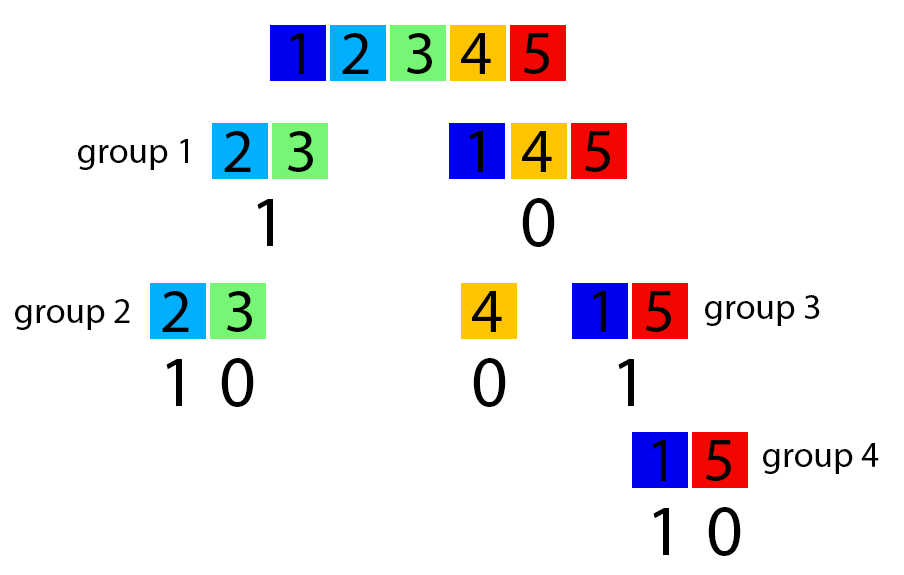
\includegraphics[width=0.6\textwidth]{capitulo_3/imagens/grouping.png}
\end{figure}

Os quatro grupos de amostras gerados a partir da regra de hierarquia são apresentados na \autoref{fig:jura_mc}. O primeiro grupo contém todas as amostras do conjunto de dados, enquanto os outros são subconjuntos.

\begin{figure}[H]
    \caption{Mapa de localização das amostras dos quatro grupos.} \label{fig:jura_mc}
     \centering
     \subfloat[][Grupo 1]{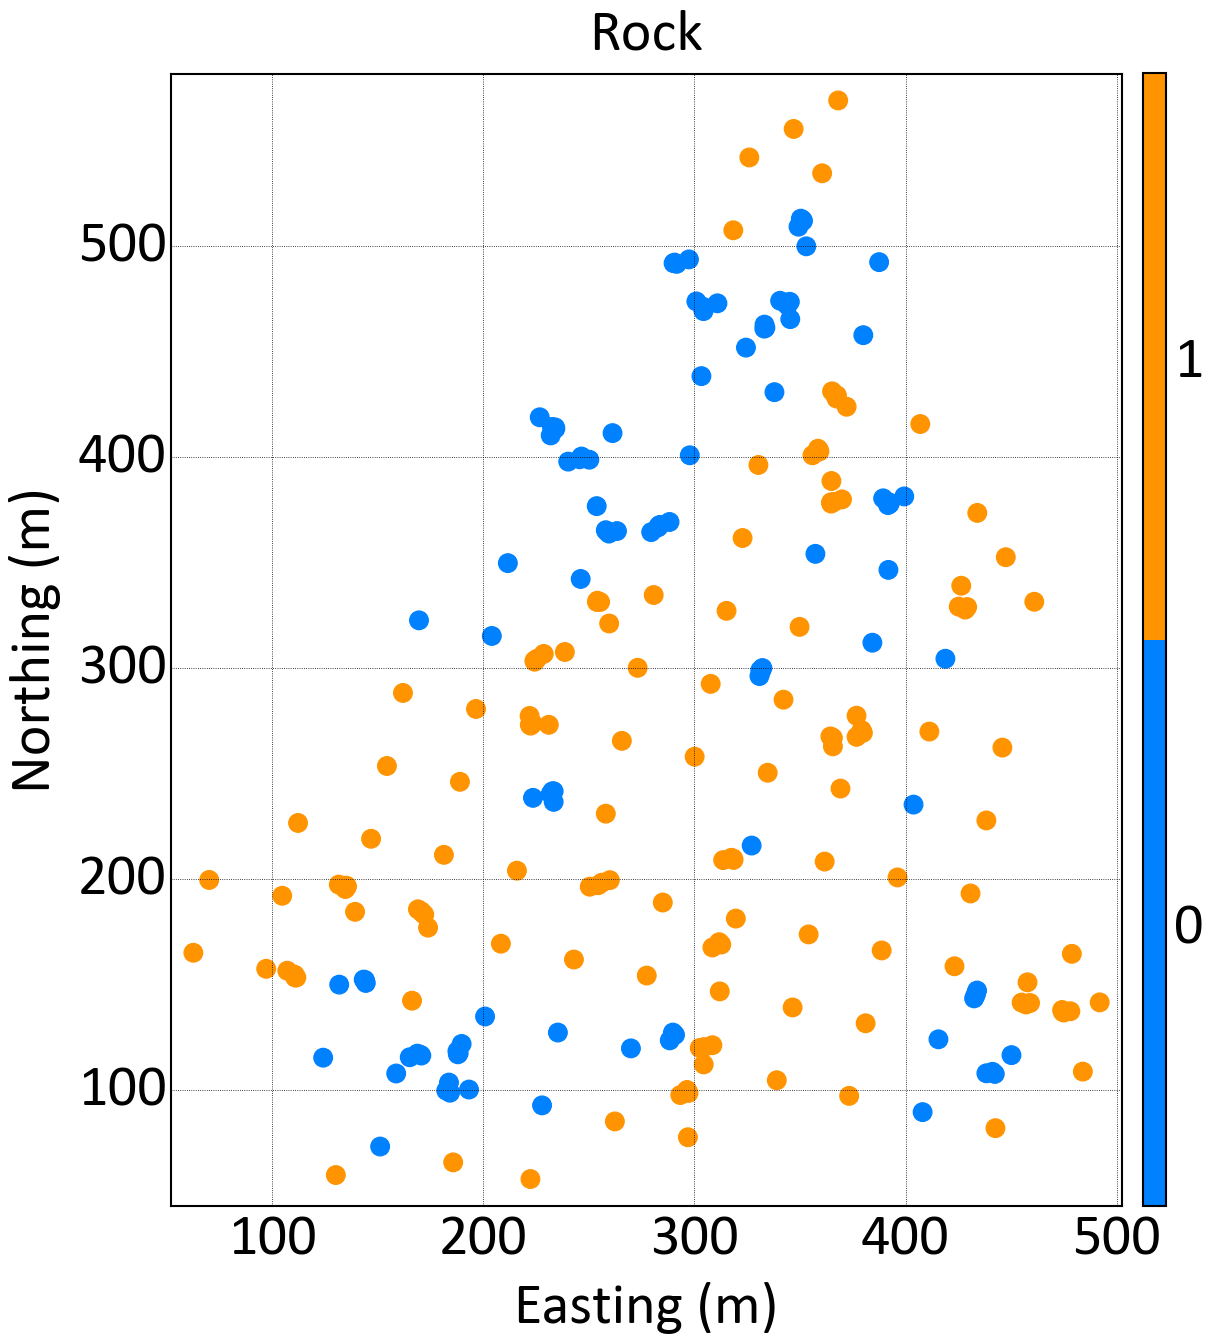
\includegraphics[height=150pt]{capitulo_3/imagens/gg1.png}\label{fig:g1}}
     \hspace{1em}
     \subfloat[][Grupo 2]{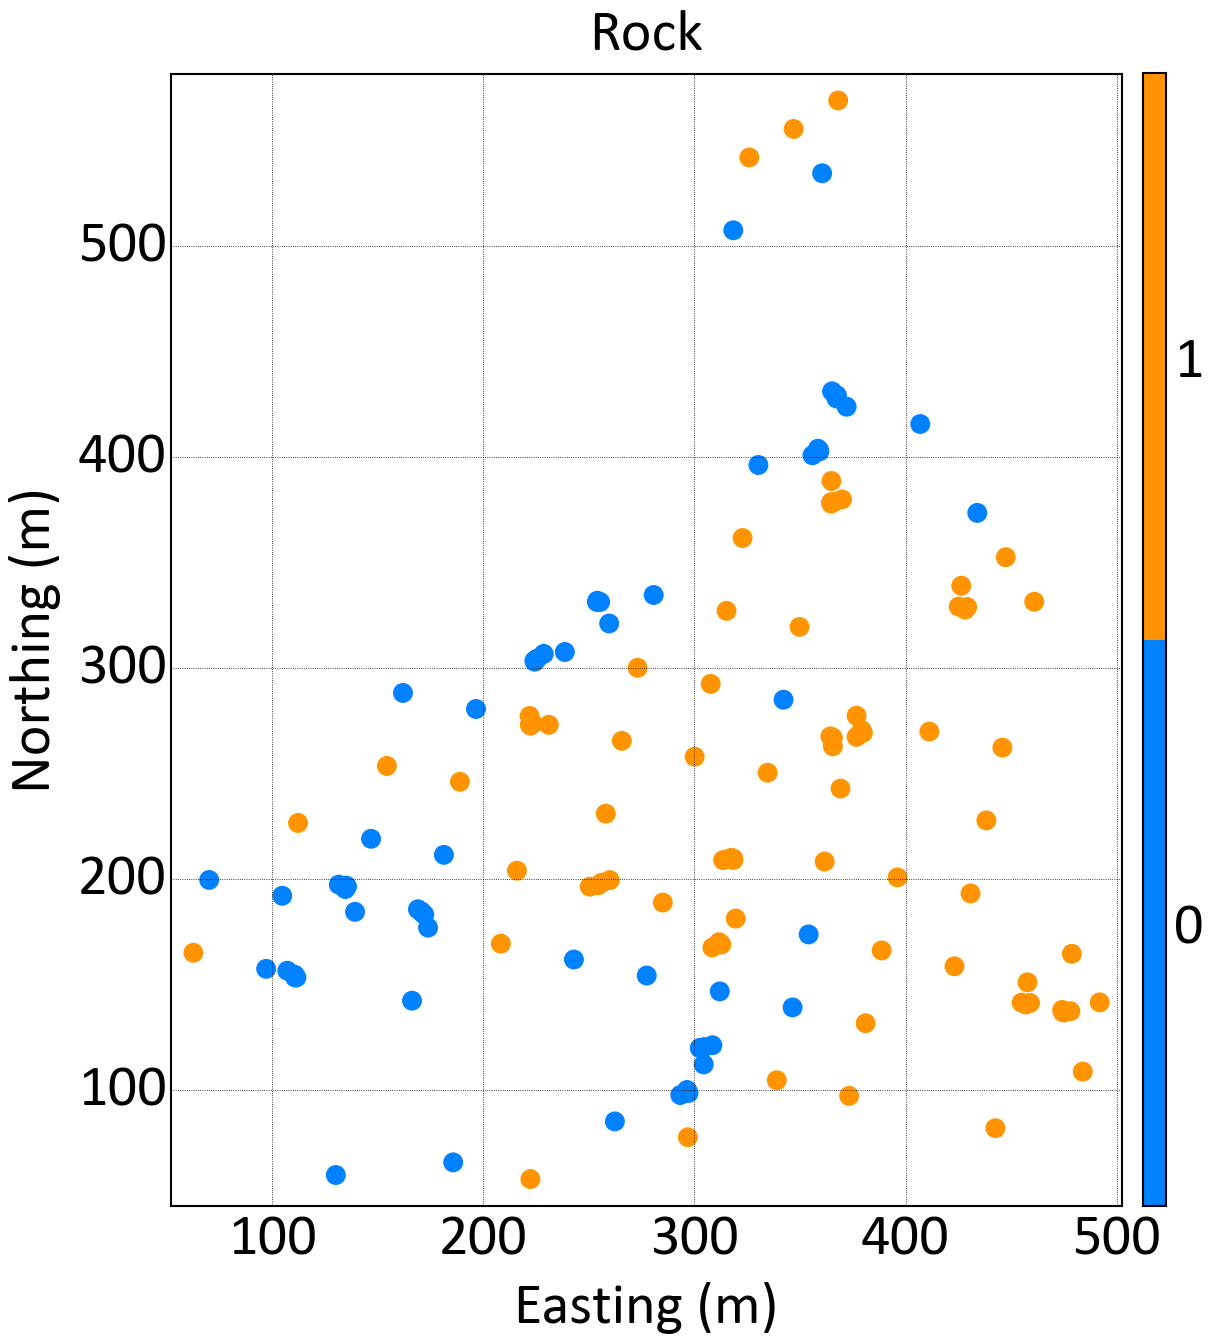
\includegraphics[height=150pt]{capitulo_3/imagens/gg2.png}\label{fig:g2}}\\
     \subfloat[][Grupo 3]{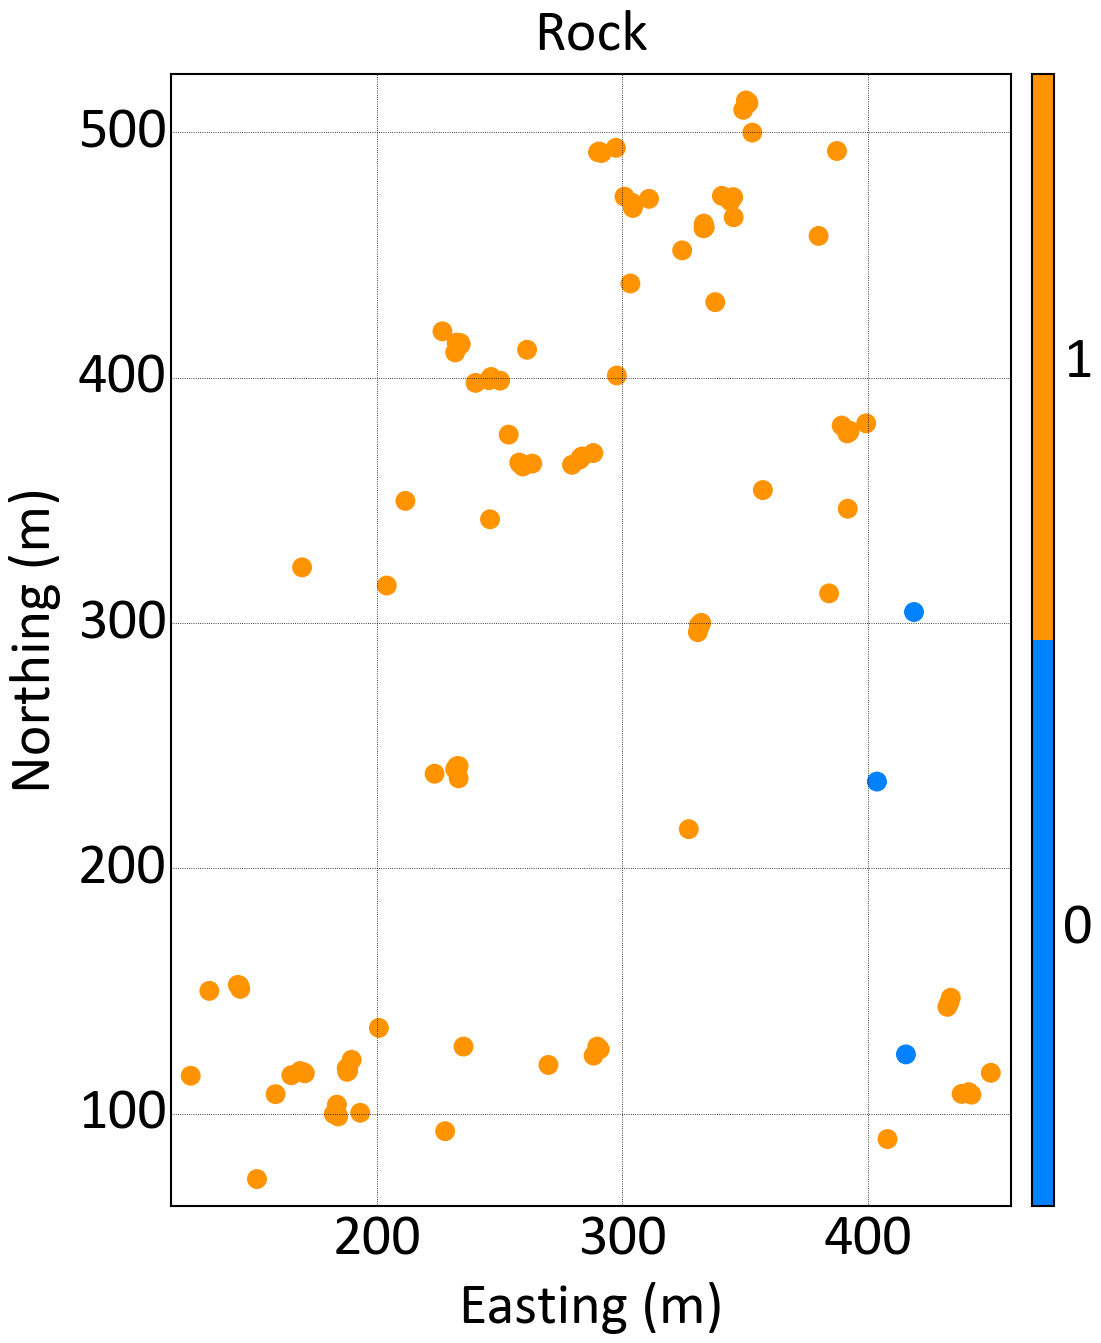
\includegraphics[height=150pt]{capitulo_3/imagens/gg3.png}\label{fig:g3}}
     \hspace{1em}
     \subfloat[][Grupo 4]{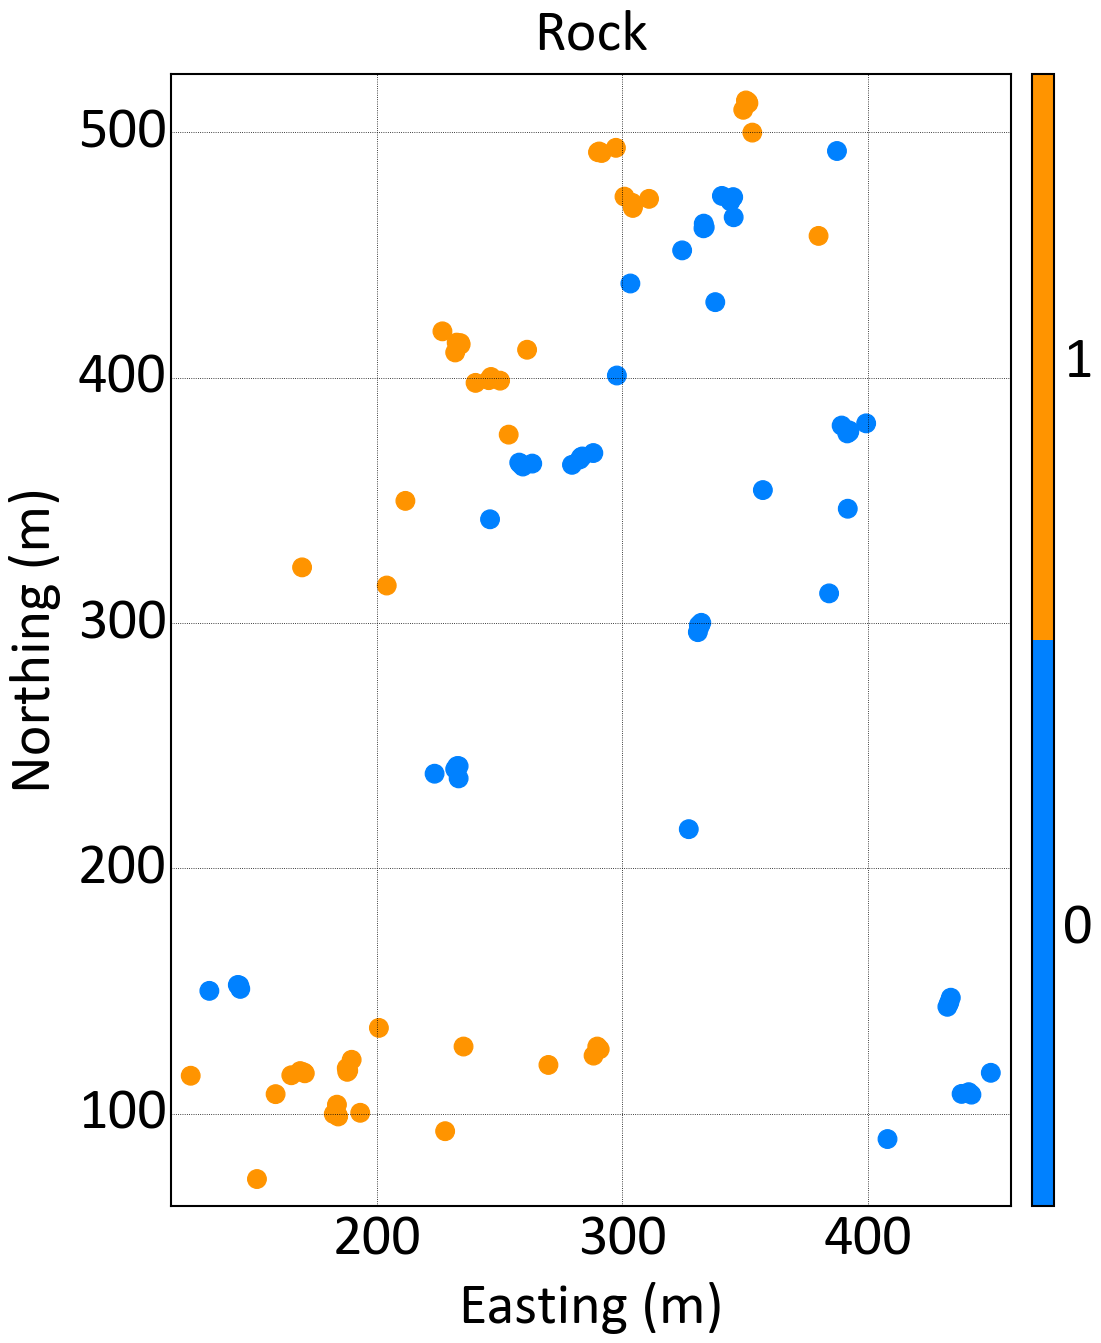
\includegraphics[height=150pt]{capitulo_3/imagens/gg4.png}\label{fig:g4}}
\end{figure}

É necessário definir uma zona de incerteza em torno dos contatos entre os indicadores de cada grupo. Blocos localizados fora da zona são considerados como pertencentes a um determinado indicador, enquanto blocos dentro da zona terão sua incerteza avaliada. A zona de incerteza é obtida usando o mesmo parâmetro C apresentado na \autoref{boundsim} para criar e controlar a largura da banda. O parâmetro C deve ser calibrado ou determinado empiricamente para cada grupo. Para o exemplo do \textit{Swiss Jura}, um valor C de 12 metros foi escolhido para todos os quatro grupos.

As propriedades funções distância assinaladas devem ser calculadas, modificadas pelo parâmetro C de acordo com a \autoref{C_dist}, e interpoladas para cada grupo. A interpolação estima para cada nó do \textit{grid} o valor da função de distância modificada. A zona de incerteza, para cada grupo, é determinada pelos blocos com valores estimados entre $ -C $ e $ + C $.

A figura \autoref{fig:jura_int} mostra as distâncias assinaladas modificadas interpoladas para cada grupo. A interpolação foi realizada em um \textit{grid} de 3x3 metros por RBF usando \textit{kernels} Gaussianos equivalentes aos variogramas dos indicadores de cada grupo.

\begin{figure}[H]
    \caption{Distâncias modificadas e interpoladas para cada um dos grupos.} \label{fig:jura_int}
     \centering
     \subfloat[][Grupo 1]{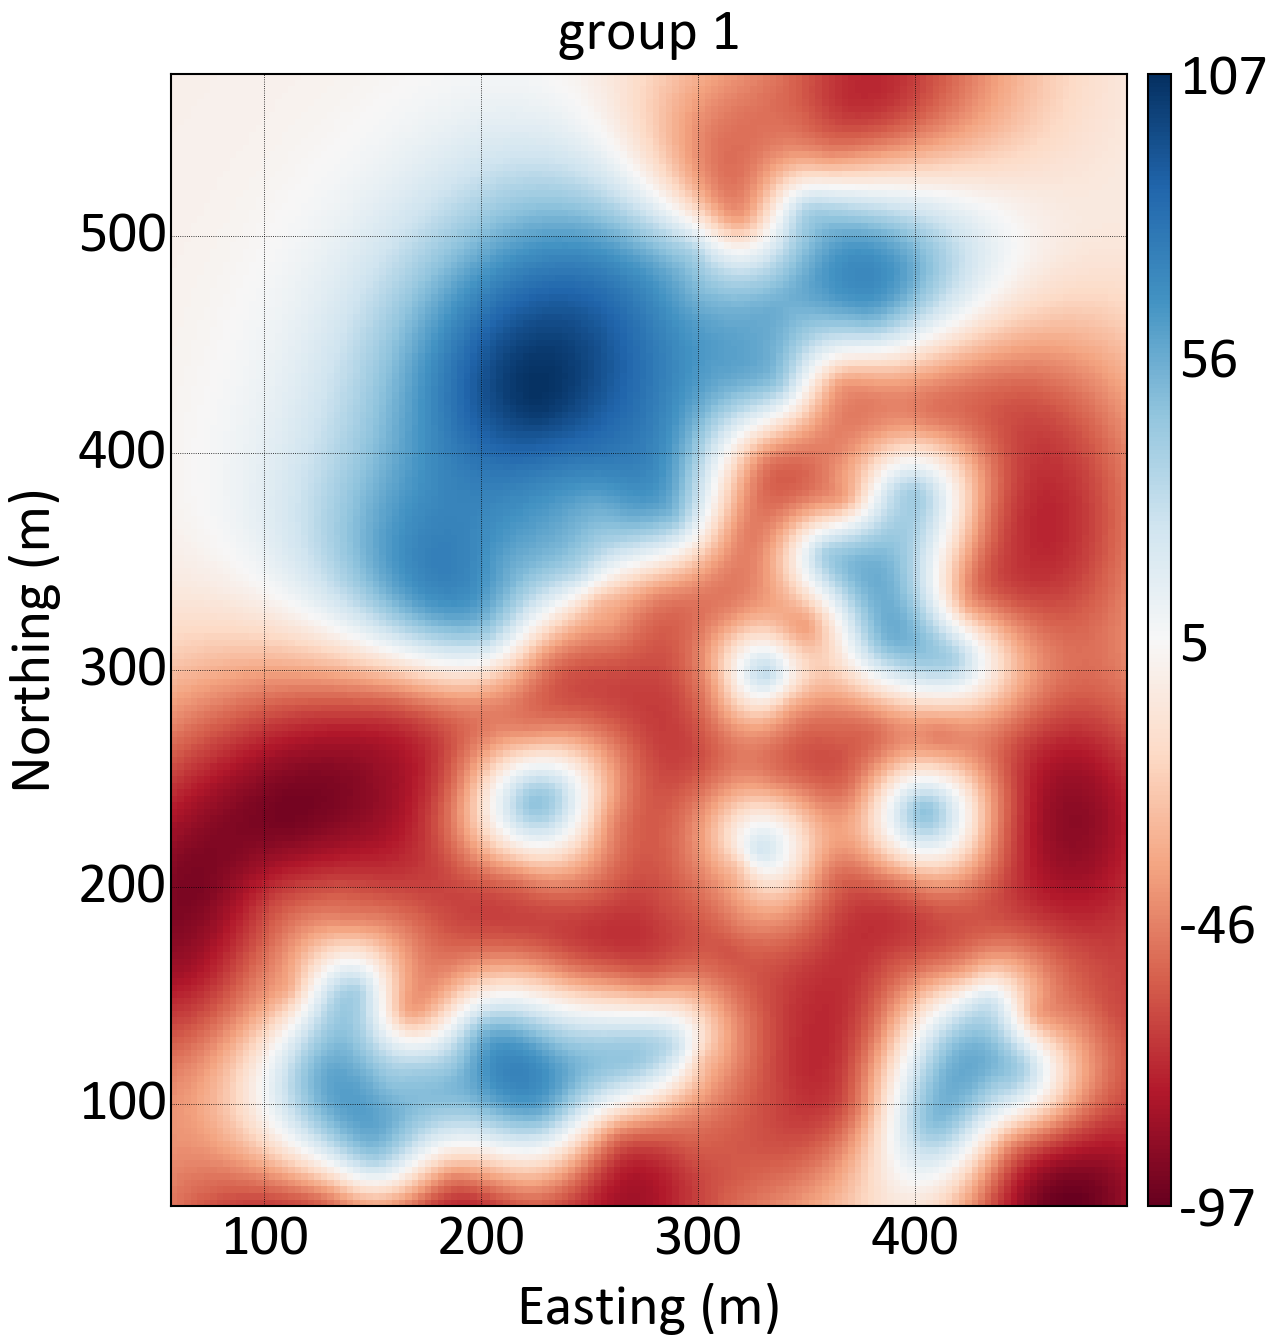
\includegraphics[height=150pt]{capitulo_3/imagens/int_g1.png}\label{fig:int1}}
     \hspace{1em}
     \subfloat[][Grupo 2]{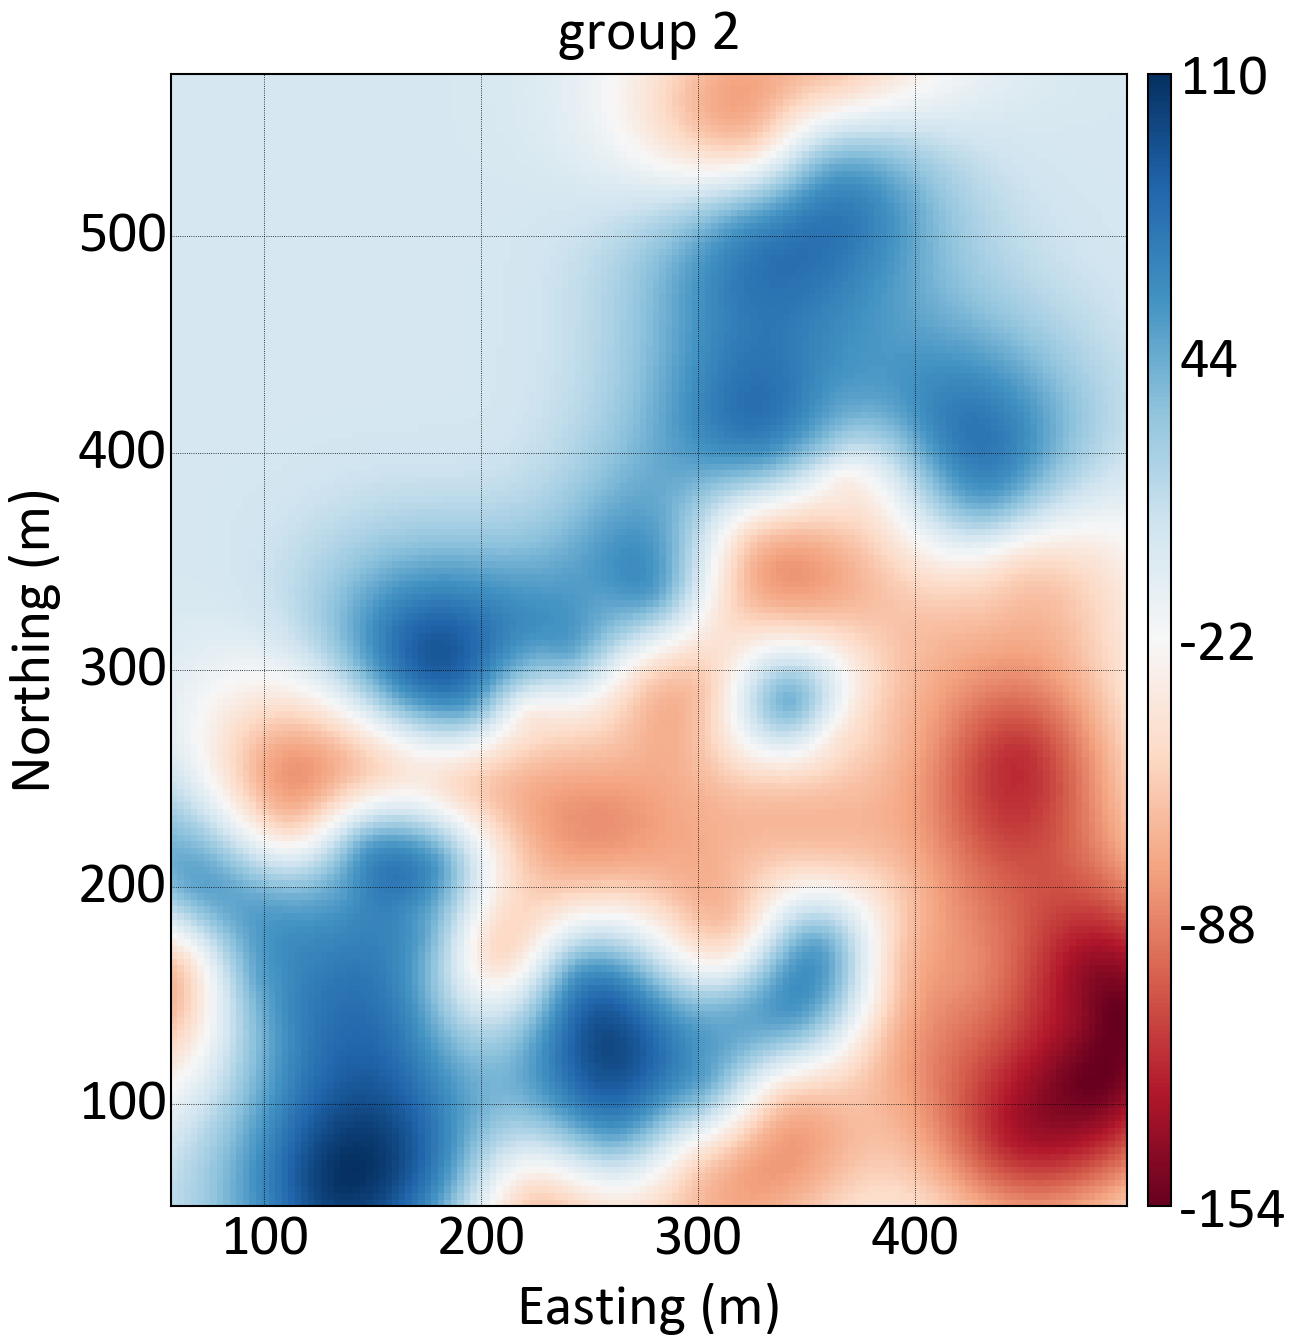
\includegraphics[height=150pt]{capitulo_3/imagens/int_g2.png}\label{fig:int2}}\\
     \subfloat[][Grupo 3]{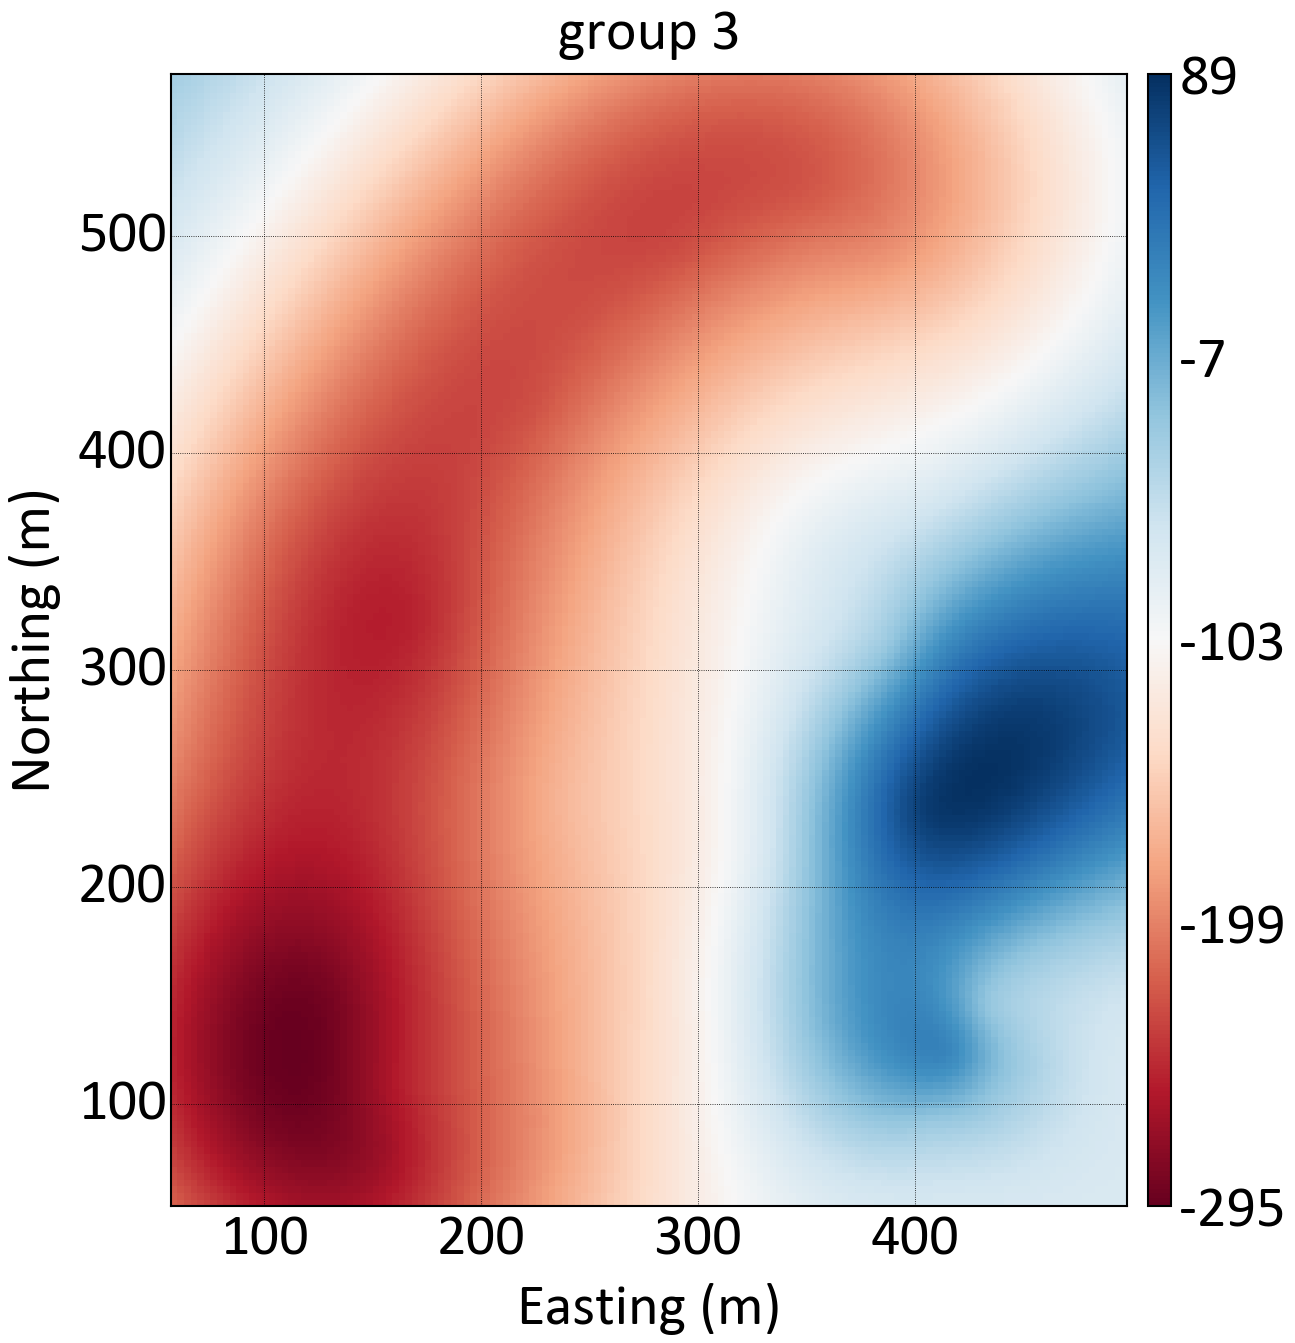
\includegraphics[height=150pt]{capitulo_3/imagens/int_g3.png}\label{fig:int3}}
     \hspace{1em}
     \subfloat[][Grupo 4]{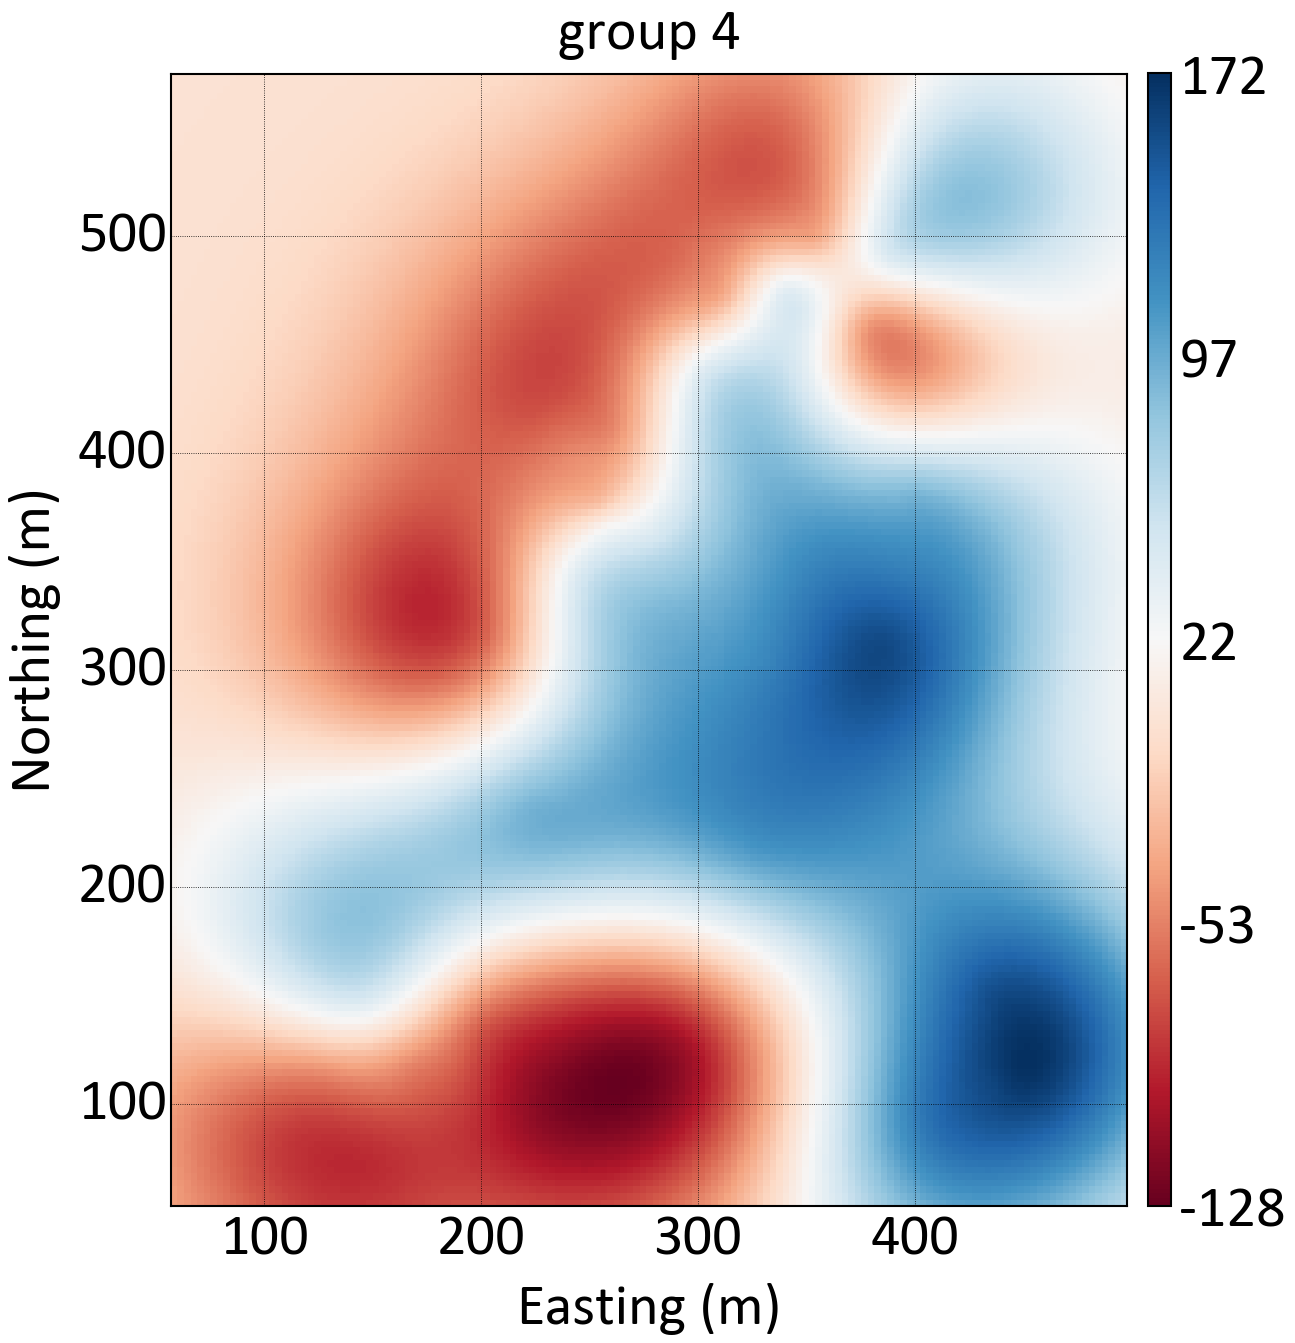
\includegraphics[height=150pt]{capitulo_3/imagens/int_g4.png}\label{fig:int4}}
\end{figure}

A figura \autoref{fig:jura_sim} apresenta, uma realização de um total de 10, dos valores Gaussianos simulados dentro da zona de incerteza para cada grupo. A zona de incerteza foi definida truncando os valores interpolados da \autoref{fig:jura_int} entre $ -C $ e $ + C $, nesse caso 12 metros.

Como um contato está sendo simulado, é recomendado o uso de um variograma Gaussiano para a simulação não condicional, pois permite que a continuidade de curto alcance seja reproduzida \cite{wilde2012kriging}. \citeonline{martin2017implicitmodeling} advoga que o mesmo variograma usado para interpolar as distâncias assinaladas deve ser usado para simular os valores Gaussianos.

\begin{figure}[H]
    \caption{Uma realização dos valores Gaussianos simulados, dentro da zona de incerteza, para cada grupo.} \label{fig:jura_sim}
     \centering
     \subfloat[][Valores Gaussianos simulados para o grupo 1.]{\includegraphics[height=150pt]{capitulo_3/imagens/jurareal1.png}\label{fig:int1}}
     \hspace{1em}
     \subfloat[][Valores Gaussianos simulados para o grupo 2.]{\includegraphics[height=150pt]{capitulo_3/imagens/jurareal2.png}\label{fig:int2}}\\
     \subfloat[][Valores Gaussianos simulados para o grupo 3.]{\includegraphics[height=150pt]{capitulo_3/imagens/jurareal3.png}\label{fig:int3}}
     \hspace{1em}
     \subfloat[][Valores Gaussianos simulados para o grupo 4.]{\includegraphics[height=150pt]{capitulo_3/imagens/jurareal4.png}\label{fig:int4}}
\end{figure}

A classificação da localização não amostrada $u$ como indicador 1 ou 0 é realizada comparando os valores interpolados $df^{*}(u)$ com os valores simulados $df'(u)$ de acordo com a \autoref{comp_class}:

A figura \autoref{fig:jura_groups} mostra uma realização dos limites simulados para cada grupo.

\begin{figure}[H]
    \caption{Uma realização da simulação de limites para todos os grupos.} \label{fig:jura_groups}
     \centering
     \subfloat[][Simulação dos limites para o grupo 1.]{\includegraphics[height=150pt]{capitulo_3/imagens/g1.png}\label{fig:int1}}
     \hspace{1em}
     \subfloat[][Simulação dos limites para o grupo 2.]{\includegraphics[height=150pt]{capitulo_3/imagens/g2.png}\label{fig:int2}}\\
     \subfloat[][Simulação dos limites para o grupo 3.]{\includegraphics[height=150pt]{capitulo_3/imagens/g3.png}\label{fig:int3}}
     \hspace{1em}
     \subfloat[][Simulação dos limites para o grupo 4.]{\includegraphics[height=150pt]{capitulo_3/imagens/g4.png}\label{fig:int4}}
\end{figure}

As realizações de cada grupo devem ser sobrepostas para gerar uma realização para o modelo geológico. A categoria correspondente deve ser atribuída a cada nó do \textit{grid} de acordo com as regras de hierarquização da Figura \autoref{fig:groups_fig}. Por exemplo, Kimmeridgian é atribuído a um nó do \textit{grid} se duas condições forem satisfeitas: o bloco pertence à região do grupo 1, classificada com o indicador 1, e pertence à região classificada com o indicador 1 no grupo 2. Da mesma forma, Argovian é atribuído a um nó do \textit{grid} se três condições forem satisfeitas: o bloco pertence à região do grupo 1, classificada com o indicador 0, o bloco pertence à região classificada com o indicador 1 no grupo 3, e o bloco pertence à região classificada com o indicador 1 em grupo 4.

A \autoref{fig:jura_reals} mostra 2, de 10 realizações, para o modelo geológico. Uma animação das 10 realizações pode ser vista \href{https://github.com/robertorolo/hierarchical_boundary_simulation/blob/main/jura_gif.gif}{aqui}.

\begin{figure}[H] 
    \centering
    \caption{Duas realizações para o modelo geológico para o \textit{Swiss Jura}.} \label{fig:jura_reals}
     \subfloat[][Realização 1.]{\includegraphics[width=.45\textwidth]{capitulo_3/imagens/geomodel_0.png}\label{<figure1>}}
     \hspace{1em}
     \subfloat[][Realização 2.]{\includegraphics[width=.45\textwidth]{capitulo_3/imagens/geomodel_1.png}\label{<figure2>}}
\end{figure}

\subsection{Estudo de caso}

Esse estudo de caso foi realizado em um depósito de cobre pórfiro para demonstrar a eficiência da metodologia proposta. O depósito mineral consiste em cinco domínios geológicos mapeados com dados de 91 furos de sondagem, que foram compositados em intervalos de 15 metros, o que leva a 3.276 amostras de suporte pontual. Três domínios são rochas intrusivas, um domínio é de rochas oxidadas e o último é de rochas sulfetadas. A \ref{fig:pointscp} mostra uma vista em perspectiva dos furos compositados. As amostras em azul escuro representam rochas sulfetadas da categoria 1; o azul claro representa a categoria 2, rochas oxidadas; e verde, amarelo e vermelho representam as categorias 3, 4 e 5 de rochas intrusivas, respectivamente.

\begin{figure}[H]
\caption{Vista em perspectiva para o conjunto de dados no suporte pontual que descreve as cinco categorias.}
\label{fig:pointscp}
\centering
\includegraphics[width=0.7\textwidth]{capitulo_3/imagens/pointscp.png}
\end{figure}

O algoritmo de agrupamento proposto foi aplicado a um proto-modelo criado usando distâncias assinaladas a partir das amostras em suporte pontual do depósito de cobre pórfiro em um \textit{grid} de 50x50x30 metros. Como resultado, a regra de hierarquia apresentada na \autoref{fig:groupingcp} é gerada. As amostras agrupadas são mostradas na \autoref{fig:cpgroups}.

\begin{figure}[H]
\caption{Regra de hierarquia para o conjunto de dados do estudo de caso definido pelo algoritmo proposto.}
\label{fig:groupingcp}
\centering
\includegraphics[width=0.6\textwidth]{capitulo_3/imagens/groupingcp.png}
\end{figure}

\begin{figure}[H]
    \caption{Visão em perspectiva para os grupos de amostras em suporte pontual.} \label{fig:cpgroups}
     \centering
     \subfloat[][Grupo 1]{\includegraphics[height=130pt]{capitulo_3/imagens/g1cp.png}\label{fig:cpgp1}}
     \subfloat[][Grupo 2]{\includegraphics[height=130pt]{capitulo_3/imagens/g2cp.png}\label{fig:cpgp2}}\\
     \subfloat[][Grupo 3]{\includegraphics[height=130pt]{capitulo_3/imagens/g3cp.png}\label{fig:cpgp3}}
     \subfloat[][Grupo 4]{\includegraphics[height=130pt]{capitulo_3/imagens/g4cp.png}\label{fig:cpgp4}}
\end{figure}

A figura \autoref{fig:cs_variograms} mostra os variogramas dos indicadores para cada grupo. Para os grupos 1, 3 e 4, um variograma omnidirecional foi calculado e modelado. Já para o grupo 2, foram calculados e modelados variogramas omni-horizontal (em azul) e vertical (em vermelho).

\begin{figure}[H]
    \caption{Variogramas dos indicadores para cada grupo.} \label{fig:cs_variograms}
     \centering
     \subfloat[][Variograma omnidirecional para o grupo 1.]{\includegraphics[width=0.45\textwidth]{capitulo_3/imagens/cp_var_1.png}\label{fig:v1}}
     \hspace{1em}
     \subfloat[][Variograma omni-horizontal em azul e vertical em vermelho para o grupo 2.]{\includegraphics[width=0.45\textwidth]{capitulo_3/imagens/cp_var_2.png}\label{fig:v2}}\\
    \subfloat[][Variograma omnidirecional para o grupo 3.]{\includegraphics[width=0.45\textwidth]{capitulo_3/imagens/cp_var_3.png}\label{fig:v3}}
    \hspace{1em}
    \subfloat[][Variograma omnidirecional para o grupo 4.]{\includegraphics[width=0.45\textwidth]{capitulo_3/imagens/cp_var_4.png}\label{fig:v4}}
\end{figure}

A calibração do parâmetro C foi realizada com 20 conjuntos de dados \textit{jackknife} aleatórios para cada grupo, removendo 10\% dos furos em cada execução, e com 30 parâmetros C aleatórios de zero a um determinado intervalo em metros para cada grupo. A calibração de C deve ser realizada para uma variedade de subconjuntos \textit{jackknife} para garantir que a calibração seja robusta \citeonline{wilde2012kriging}. Os resultados são mostrados na \autoref{fig: uncert_groups}.

A diretriz para escolher um parâmetro C para cada grupo a partir do índice de classificação incorreta nas calibrações mostradas em \autoref{fig:uncert_groups} é considerar uma taxa de classificação incorreta aceitável. Valores razoáveis para os parâmetros C foram escolhidos para cada grupo com base nos resultados da calibração, o tipo de depósito e a configuração dos dados.

Os valores escolhidos foram 5\%, 0,5\%, 2,5\% e 10\% de taxas de classificação incorreta aceitáveis para os grupos 1, 2, 3 e 4, respectivamente, que correspondem aos valores dos parâmetros C de 170m, 30m, 50m e 200m. A escolha do parâmetro C da calibração \textit{jackknife} é subjetiva, no entanto, a calibração auxilia o geomodelador na escolha de um valor adequado para o parâmetro. Um valor de C não deve ser escolhido na região onde a curva se torna horizontal. Além disso, a largura de banda da incerteza não pode ser maior que o espaçamento do furo de sondagem \citeonline{rossi2013mineral}.

\begin{figure}[H]
    \caption{Calibração do parâmetro C por \textit{jackknife}} \label{fig:uncert_groups}
     \centering
     \subfloat[][Grupo 1]{\includegraphics[height=120pt]{capitulo_3/imagens/uncert_g1.png}\label{fig:r1cp}}
     \subfloat[][Grupo 2]{\includegraphics[height=120pt]{capitulo_3/imagens/uncert_g2.png}\label{fig:r2cp}}\\
    \subfloat[][Grupo 3]{\includegraphics[height=120pt]{capitulo_3/imagens/uncert_g3.png}\label{fig:r3cp}}
     \subfloat[][Grupo 4]{\includegraphics[height=120pt]{capitulo_3/imagens/uncert_g4.png}\label{fig:r4cp}}
\end{figure}

As funções distância calculadas para cada grupo foram modificadas com o parâmetro C escolhido, adicionando C às amostras codificadas como 0 e subtraindo C das amostras codificadas como 1. As distâncias modificadas para cada grupo foram então interpoladas para todos os nós do \textit{grid}. As funções de base radial foram escolhidas para interpolar a função distância para um \textit{grid} com dimensões de bloco de 25x25x15 metros. O \textit{kernel} RBF é Gaussiano com efeito pepita de 0,001\% para evitar instabilidades nas matrizes. O suporte dos \textit{kernels} é o alcance dos variogramas dos indicadores de cada grupo (\autoref{fig:cs_variograms}). As razões de anisotropia de cada grupo também foram consideradas.

A zona de incerteza é obtida a partir dos modelos implícitos interpolados, truncando-os entre $-C$ e $+C$. Simulações não condicionais foram realizadas nesta região, e cada realização das simulações é transformada para que seus valores estejam entre $-C$ e $+ C$ a partir da \autoref{sim_trans}. Equivalentes Gaussianos aos variogramas dos indicadores foram utilizados para simular cada um dos grupos. Dez realizações foram geradas para cada grupo comparando o valor simulado com os valores interpolados dentro da zona de incerteza. 

As realizações para cada grupo devem ser sobrepostas, respeitando a regra de hierarquização da \autoref{fig:groupingcp}, para gerar uma realização para o modelo geológico. Além disso, as realizações são mescladas respeitando seu índice. A realização 2 obtida na simulação de cada grupo é usada para construir a realização 2 do modelo geológico hierárquico.

A \autoref{cobre_reals} mostra uma seção vertical e uma horizontal para duas realizações do modelos geológico juntamente com os dados amostrais em suporte pontual. Uma animação mostrando seções verticais em XZ das 10 realizações executadas pode ser vista \href{https://github.com/robertorolo/hierarchical_boundary_simulation/blob/main/copper_gif.gif}{aqui}.

\begin{figure}[H]
	\caption{\label{cobre_reals} Visão em perspectiva de seções verticais e horizontais de duas realizações do modelo geológico juntamente com as amostras em suporte pontual.}
	\centering
		\subfloat[][Realização 1]{\includegraphics[width=0.45\textwidth]{capitulo_3/imagens/real0cp.png}\label{fig:g1}}
     \hspace{1em}
     \subfloat[][Realização 2]{\includegraphics[width=0.45\textwidth]{capitulo_3/imagens/real1cp.png}\label{fig:g2}}
\end{figure}

\subsection{Discussão}

A SISIM foi aplicada ao mesmo banco de dados, assim como na \autoref{pfiels}, a fim de comparar os resultados com a metodologia proposta. Os variogramas dos indicadores para as cinco categorias foram calculados e modelados, e os indicadores foram simulados para o mesmo \textit{grid} em que a simulação de contatos hierárquica foi realizada. A \autoref{fig:sisimsec} mostra as mesmas 4 seções verticais ao longo de XZ comparando uma realização da SISIM com a metodologia proposta. A SISIM gera um modelo com uma textura \textit{“salt and pepper”} e padrões ruidosos, que não são geologicamente realistas. A simulação hierárquica de contatos (Figura \autoref{fig:r2cp}) gera limites contínuos, eologicamente realistas, que honram os dados, como mostra a matriz de confusão na \autoref{fig:backflag_bound_hier}. Além disso, apenas 4 variogramas dos indicadores, um para cada grupo, devem ser calculados e modelados, contra 5 variogramas para a SISIM. Como o RBF é um interpolador global, os parâmetros da vizinhança de busca não devem ser configurados, ao contrário da SISIM. Como desvantagens, esse algoritmo também não possui mecanismo para respeitar as proporções e reproduzir a continuidade espacial de cada categoria, embora isso possa ser contornado alterando iterativamente os parâmetros e verificando os resultados.

\begin{figure}[H]
    \caption{Seções equidistantes em XZ comparando uma realização do modelo geológico do SISIM com uma realização da metodologia proposta.} \label{fig:cs_reals}
     \centering
     \subfloat[][SISIM.]{\includegraphics[width=0.45\textwidth]{capitulo_3/imagens/cp_sisim_real_0.png}\label{fig:sisimsec}}
     \hspace{1em}
     \subfloat[][Simulação hierárquica de contatos.]{\includegraphics[width=0.45\textwidth]{capitulo_3/imagens/real_0.png}\label{fig:r2cp}}
\end{figure}

Uma forma quantitativa de avaliar a incerteza de modelos geológicos é usando a entropia de informação, essa técnica tem sido aplicada em geociências como uma medida de qualidade de modelos geológicos \cite{yang2019assessing}. A \autoref{fig:cs_entropy} mostra a entropia da informação calculada para a SISIM e para a metodologia proposta. Como esperado, na metodologia proposta os maiores valores de entropia da informação estão em torno dos contatos, ao contrário da SISIM, onde altos valores de entropia estão espalhados no espaço. A maior parte da incerteza reside em áreas onde várias categorias têm uma alta probabilidade de ocorrência. Essa análise é necessária porque ao contrário do método apresentado na \autoref{pfiels}, onde é criada uma zona de incerteza ao redor dos contatos entre as litologias, nesse caso a zona de incerteza é criada ao redor dos contatos dos grupos definidos, portanto, é necessário verificar se no modelo geológico a incerteza reside, de fato, ao redor dos contatos entre as litologias.

\begin{figure}[H]
    \caption{Seções equidistantes em XZ comparando a entropia do SISIM com uma realização da metodologia proposta.} \label{fig:cs_entropy}
     \centering
     \subfloat[][Entropia para a SISIM.]{\includegraphics[width=0.45\textwidth]{capitulo_3/imagens/sisim_entropy.png}\label{fig:ent1}}
     \hspace{1em}
     \subfloat[][Entropia para a simulação hierárquica de contatos.]{\includegraphics[width=0.45\textwidth]{capitulo_3/imagens/hierbound_entropy.png}\label{fig:ent2}}
\end{figure}

\begin{figure}[H]
	\caption{\label{fig:backflag_bound_hier} Matriz de confusão mostrando a média da proporção de blocos que reproduzem as amostras mais próximas entre todas as realizações para todas as categorias do banco de dados.}
	\centering
		\includegraphics[width=0.6\textwidth]{capitulo_3/imagens/backflag_bound_hier.png}
\end{figure}

Os parâmetros do \textit{grid} de simulação podem ser predeterminados pelos requisitos de engenharia para um determinado projeto. No entanto, as definições do \textit{grid} para o modelo geológico não precisam corresponder às da modelagem numérica; a consideração mais importante é a capacidade de reproduzir as menores feições geológicas de interesse \cite{martin}. O parâmetro C e a resolução do \textit{grid} devem ser compatíveis, se o parâmetro C for maior que as dimensões da célula, a zona de incerteza pode ter poucos blocos ou até mesmo nenhum.

Os parâmetros do variograma de interpolação, a saber, alcance, anisotropia e efeito pepita, controlam a forma e o volume das diferentes categorias. Existe uma estreita relação entre o variograma utilizado para a interpolação de cada grupo e o parâmetros C. O mesmo valor para C pode levar a uma zona de incerteza maior se o alcance do variograma aumentar.

O comportamento dos contatos é controlado pelo variograma usado na simulação não condicional, alcances menores e efeitos pepita maiores geram limites ásperos e descontínuos, por outro lado, alcances longos e efeitos pepita pequenos geram limites suaves e contínuos.

A magnitude da incerteza pode ser controlada pelo parâmetro C, que define a largura da banda da incerteza. O parâmetro C pode ser calibrado a partir dos dados existentes ou determinado por um especialista, com base no conhecimento sobre o depósito, a largura da banda de incerteza não deve ser nem muito grande nem muito pequena, o verdadeiro limite entre domínios deve existir em algum local no interior da zona de incerteza. A variação do volume de cada litologia depende diretamente do parâmetro C definido para cada grupo. A Figura \autoref{fig:sensibilidade_c} mostra a entropia da informação calculada para o exemplo no\textit{Swiss Jura} com diferentes valores para C. A Figura \autoref{fig:c1} mostra o caso base, onde os valores de C para todos os grupos são iguais a 12 metros, a figura \autoref{fig:c2} mostra a entropia da informação para valores de C igual a 60 metros para todos os grupos, a largura da banda da incerteza é maior do que o caso base. Finalmente, a Figura\autoref{fig:c3} mostra um caso onde o parâmetro C é igual a 12 metros para os grupos 1, 2 e 3 e 60 metros para o grupo 4. Como o grupo 4 representa o contato entre as categorias Argovian e Quaternary, a zona de incerteza é maior em torno desses contatos do que nos demais.

\begin{figure}[H]
    \caption{Efeito do parâmtro C.} \label{fig:sensitivity_c}
     \centering
     \subfloat[][grupo 1: 12m; grupo 2: 12m; grupo 3: 12m; grupo 4: 12m ]{\includegraphics[height=120pt]{capitulo_3/imagens/jura_entropy.png}\label{fig:c1}}
     \hspace{1em}
     \subfloat[][grupo 1: 60m; grupo 2: 60m; grupo 3: 60m; grupo 4: 60m]{\includegraphics[height=120pt]{capitulo_3/imagens/jura_entropy_60_60_60_60.png}\label{fig:c2}} \\
     \subfloat[][grupo 1: 12m; grupo 2: 12m; grupo 3: 12m; grupo 4: 60m]{\includegraphics[height=120pt]{capitulo_3/imagens/jura_entropy_12_12_12_60.png}\label{fig:c3}}
\end{figure}

Vale ressaltar que a principal desvantagem do método consiste em determinar as regras de hierarquia. O algoritmo proposto automatiza o processo, entretanto, a resolução do \textit{grid} do proto-modelo e o método utilizado para criar o proto-modelo podem produzir diferentes agrupamentos. A hierarquia entre as categorias pode ser determinada cronologicamente por um geomodelador. No entanto, essa escolha depende do conhecimento sobre o depósito mineral e da experiência do geomodelador. Também pode ser determinado de forma arbitrária, o que pode levar a modelos geológicos subjetivos, irreproduzíveis e não auditáveis.